% ==========================
%  LaTeX 2e - Dokument
%  Editor: Dragan Kozulovic
% ==========================
\documentclass[11pt,a4paper,fleqn,twoside]{report}
\usepackage[dvips,final]{graphicx}               %% epsfig -> tex-bilder
\usepackage[latin1]{inputenc}                    %% ISO-Text mit Umlauten
\usepackage[T1]{fontenc}                         %% Zeichensatz mit Umlauten
%\usepackage[lflt]{floatflt}                     %% Textfluss um Bilder
\usepackage[german]{babel}                       %% BABEL -> deutsch
\usepackage{parskip}                             %% parindent=0 / parskip
\usepackage{fancyhdr}                            %% 'fancy'-Ueberschriften
\usepackage[hang,bf]{caption}                    %% Formatierung der captions
\usepackage{color}                               %% Farben
\usepackage{multirow}                            %% Tabellen
\usepackage{natbib}
\usepackage{pdfpages}							 %% PDF ins Dokument integrieren
\usepackage{amsmath}                   			 %% Packages f�r Formeln
\usepackage{amsthm}								 %% -||-
\usepackage{amsfonts}							 %% -||-
\usepackage{amssymb} 							 %% -||-
\usepackage{siunitx}							 %% SI-Einheiten
\usepackage{booktabs}          					 %%table \toprule \bottomrule \midrule
\usepackage{subcaption}
\captionsetup[subfigure]{list=true, font=large, labelfont=bf, 
	labelformat=brace, position=top}
\usepackage[onehalfspacing]{setspace}
\usepackage{float}

% Einzubindende Dateien 
\includeonly{00_frontpage,
             00_empty_page,
	     00_eid_erkl,
	     00_abstract,
	     00_nomenklatur,
	     01_einleitung,
	     02_grundlagen,
	     03_versuchsvorbereitung,
	     04_widerstandsbestimmung,
	     05_windkanalversuche,
	     06_versuchsauswertung,
	     07_fazit,
	     anhang1,
	     anhang2}
\graphicspath{{figures/}}                         %% Pfad fuer einzubindende Graphiken


% Seiten-Layout
\oddsidemargin   0.0cm                           %% Anpassung DIN A4-Format (symmetrisch)
\evensidemargin  0.0cm                           %% Anpassung DIN A4-Format (symmetrisch)
\topmargin      -1.0cm         
\textheight     25.0cm
\textwidth      16.0cm
\pagestyle{fancy}
\renewcommand{\chaptermark}[1]{\markboth{\thechapter.\ #1}{}}
\renewcommand{\sectionmark}[1]{\markright{\thesection\ #1}}
\fancyhf{}                                %Clears all header and footer fields, in preparation.
\fancyhead[LE,RO]{\thepage}               %Displays the page number in bold in the header,
                                          % to the left on even pages and to the right on odd pages.
\fancyhead[RE]{\nouppercase{\leftmark}}   %Displays the upper-level (chapter) information---
                                          % as determined above---in non-upper case in the header, to the right on even pages.
\fancyhead[LO]{\rightmark}                %Displays the lower-level (section) information---as
                                          % determined above---in the header, to the left on odd pages.
\renewcommand{\headrulewidth}{0.5pt}      %Underlines the header. (Set to 0pt if not required).

%\sloppy                                         %% lockerer Zeilenumbruch
%\flushbottom                                    %% buendige letzte Zeile


% Trennungskorrekturen
\hyphenation{Auf-triebs-pro-ble-me}
%\hyphenation{}
%\hyphenation{}


% Umbenennungen (babel) (siehe LaTeX-Begleiter, Abschn. 9.2.3)
%\addto\extrasgerman{\renewcommand{\figurename}{Abb.}}


% Listen
\newcommand{\bl}{\begin{list}{\textbullet}%         %% kleine Aufzaehlung/Liste
{\topsep0pt\partopsep0pt\itemsep0pt\parsep0pt\leftmargin1.5em\labelwidth1em\labelsep0.5em}}
\newcommand{\el}{\end{list}}
\newcommand{\cit}[1]{\textit{\cite{#1}}}

%Makros f�r eine erleichterte Eingabe wiederkehrender Befehle:
\newcommand{\abb}[1]{Abbildung~\ref{#1}}   
\newcommand{\tab}[1]{Tabelle~\ref{#1}} 
\newcommand{\glg}[1]{Gleichung~\ref{#1}}
\newcommand{\kap}[1]{Kapitel~\ref{#1}}
\newcommand{\abschn}[1]{Abschnitt~\ref{#1}}
\newcommand{\anh}[1]{Anhang~\ref{#1}}



\begin{document}
% Titelseite
\begin{titlepage}
 \centering

\begin{table}[htbp]
 \begin{center}
 \vspace{-0.5cm}
% \renewcommand{\arraystretch}{1.5}
  \begin{tabular}{lcr} 
    \parbox{0.45\textwidth}{\mbox{ }} & \parbox{0.13\textwidth}{\mbox{ }} & \parbox{0.45\textwidth}{\mbox{ }} \\
    \hspace*{-2.0cm}
    
\includegraphics[width=0.42\textwidth]{./figures/TUBraunschweig_4C.pdf} & 
     &  \\ %empty
  \end{tabular}
 \end{center}
\end{table}


 \vspace*{2.0cm}

 \textbf{\large Projektarbeit}


 \vspace*{1.5cm}
 
 \textbf{\LARGE Experiment am D-f"ormigen Stumpfk"orper} \\[0.5ex]
 


 \vspace*{1.5cm}

 \textbf{\large Nora M. Bierwagen} \\
 \textbf{\large Tim Gotzel} \\
 \textbf{\large Amiriman Kianfar} \\
 \textbf{\large Kebria Kiani} \\
 \textbf{\large Florian Timm} \\


 \vspace*{7.0cm}

 \begin{table}[htbp]
  \begin{center}
%  \renewcommand{\arraystretch}{1.5}
   \begin{tabular}{rl} 
     \parbox{0.33\textwidth}{\mbox{ }} & \parbox{0.66\textwidth}{\mbox{ }} \\
     Ausgegeben:%& Jun.-Prof. Dr.-Ing. D. Ko{\v z}ulovi{\' c} \\
                 & Institut f\" ur Str\" omungsmechanik \\
                 & Institutsleiter: Prof. Dr.-Ing. R. Radespiel \\
                 & Technische Universit\" at Braunschweig \\
                 &  \\
       Betreuer: %& Dipl.-Ing. X Y, (externe Firma) \\
                 & M.Sc. Philipp Oswald, (TU Braunschweig) \\
           %      &  \\
 %(Erstellt bei:) & (Externe Firma, Stadt) \\
                 &  \\
 Ver"offentlichung: & \today \\
   \end{tabular}
  \end{center}
 \end{table}



\end{titlepage}


%only blank page
\newpage
\thispagestyle{empty}
\mbox{}


\pagenumbering{roman}\setcounter{page}{1} 


%% Eidesstattliche Erklaerung (fuer DA, MA und BA)
%\chapter*{Eidesstattliche Erkl"arung}\label{s:eid_erkl}

Wird eine eidesstattliche Erkl"arung ben"otigt?


%Hiermit erkl"are ich, Vorname Familienname, geb. am xx.yy.zzzz, des Eides
%statt, die vorliegende Diplom-/Master-/Bachelor-Arbeit selbstst"andig und ohne
%fremde Hilfe verfasst und keine anderen als die angegebenen Hilfsmittel verwendet zu
%haben.
%
%\vspace*{3cm}
%Braunschweig, xx.yy.zzzz




%\include{empty_page}


% Uebersicht
\chapter*{Zusammenfassung}\label{s:uebersicht}

In dieser Arbeit wird die m"ogliche Widerstandsreduktion an einem D-f"ormigen Stumpfk"orper durch eine periodische hybride Aktuationsmethode untersucht und mit der konstanten Aktuation auch in Hinsicht auf eine Nettoleistungsersparnis verglichen.
Die aktive Str"omungseeinflussung kombiniert dabei die Grenzschichtbeeinflussung durch sich drehende, gezahnte Zylinder mit der Ausblasung von Coand\^{a}-Jets an der Hinterkante des Modells.

Es kann eine Widerstandsreduktion durch die periodische Aktuation im Bereich der nat"urlichen Abl"osefrequenz des K"orpers beobachtet werden.

Allerdings werden die Ergebnisse und Leistungskoeffizienten durch einige sch"adliche Effekte in ihrer Aussagekraft beeintr"achtigt, sodass weitere Untersuchungen zu dem Thema vonn"oten sind.

%only blank page
\newpage
\thispagestyle{empty}
\mbox{}



% Inhaltsverzeichnis
\fancyhead[RE]{Inhaltsverzeichnis}
\fancyhead[LO]{Inhaltsverzeichnis}
{ 
   \renewcommand{\baselinestretch}{0.8}    %% Zeilenabstand / TOC
   \small\normalsize                        %% neuen Zeilenabstand aktivieren
   \tableofcontents
}
% ATTENTION: comment out if contents sides are even number
%%only blank page
\newpage
\thispagestyle{empty}
\mbox{}



% Nomenklatur
\newpage
\fancyhead[RE]{Nomenklatur}
\fancyhead[LO]{Nomenklatur}
\chapter*{Nomenklatur}
\addcontentsline{toc}{chapter}{Nomenklatur}


\subsection*{Lateinische Bezeichnungen}
\begin{tabbing}
\hspace*{2cm}\=\kill
%$AVDR$ \> axiales Stromdichteverh\"altnis \\[0.2ex]
$Str$ \> Strouhal-Zahl \\[0.2ex]
\end{tabbing}



\subsection*{Griechische Bezeichnungen}
\begin{tabbing}
\hspace*{2cm}\=\kill
%$\beta$ \> Winkel in Umfangsrichtung \\[0.2ex]
\end{tabbing}



\subsection*{Indizes}
\begin{tabbing}
\hspace*{2cm}\=\kill
%$ax$ \> in axiale Richtung \\[0.2ex]
\end{tabbing}



\subsection*{Abk\"urzungen}
\begin{tabbing}
\hspace*{2cm}\=\kill
%$CFD$ \> \underline{C}omputational \underline{F}luid \underline{D}ynamics \\[0.2ex]
$NB$ \> \underline{N}ora M. \underline{B}ierwagen \\[0.2ex]
$TG$ \> \underline{T}im \underline{G}otzel \\[0.2ex]
$AK$ \> \underline{A}miriman \underline{K}ianfar \\[0.2ex]
$KK$ \> \underline{K}ebria \underline{K}iani \\[0.2ex]
$FT$ \> \underline{F}lorian \underline{T}imm \\[0.2ex]
%$MATLAB$ \> kommerzielle Software zur L"osung mathematischer Probleme\\[0.2ex]
$rpm$ \> Umdrehungen pro Minute \\[0.2ex]
\end{tabbing}




% alle Kapitel
\pagenumbering{arabic}\setcounter{page}{1}
\fancyhead[RE]{\nouppercase{\leftmark}}
\fancyhead[LO]{\rightmark}
\chapter{Einleitung}\label{s:einleitung}

kurze Einleitung Stumpfk"orper\\
aufbauend auf Masterarbei\\
Ziel der Arbeit\\

Da es sich bei diesem Dokument um eine Projektarbeit handelt, an der insgesamt f"unf Personen mitgewirkt haben, stehen hinter jeder Kapitel- bzw. Unterkapitel"uberschrift die Initialen des Autors. In \tab{tab:initialien} ist eine Aufschl"usselung der Initialien gegeben.

\begin{table}[h]
	\centering
	\begin{tabular}{lr}
		\toprule
		Name & Initialien\\
		\midrule
		Nora M. Bierwagen & NB\\
		Tim Gotzel & TG\\
		Amiriman Kianfar & AK\\
		Kebria Kiani & KK\\
		Florian Timm & FT\\
		\bottomrule
	\end{tabular}
	\caption{Initialien der beteiligten Personen}
	\label{tab:initialien}
\end{table}

\chapter{Grundlagen}\label{s:grundlagen}

\section{Stumpfk\"orperaerodynamik (TG)}

%	Stumpfkörper
%	D-Stumpfkörper
%	Strömungsfeld
%	Ablösung
%	Totwasser
%	Wirbelschichten
%	Nachlauf
%	Praktische Bedeutung
%	Ggf. Vergleich schlanke Körper

Im folgenden Kapitel wird der Begriff der Stumpfk"orper in Abgrenzung zu den schlanken K"orpern eingef"uhrt. Eine klare Abgrenzung von schlanken K"orpern zu Stumpfk"orpern bereitet Schwierigkeiten, da der "Ubergang oftmals flie\ss{}end ist. Jedoch unterscheidet sich das Str"omungsbild markant, weswegen im folgenden Kapitel im Besonderen auf das Str"omungsfeld und die Charakteristiken des Nachlaufs eingegangen werden sollen.

\subsection{Geometrische Einordnung}
\label{sec:Geometrie}
Ein stumpfer K"orper in einer Anstr"omung differenziert sich geometrisch von einem schlanken insofern, dass er eine signifikante Dicke quer zur Anstr"omung aufweist, welche in vergleichbarer Gr"o\ss{}enordnung wie die Abmessungen parallel zur Anstr"omung liegt. Als Ma\ss{} kann das Dickenverh"altnis $\sigma$ als Kehrwert des Schlankheitsgrades $\lambda$ herangezogen werden, welches das Verh"altnis von Dicke zu Breite wiedergibt:

\begin{align}
\sigma = \frac{1}{\lambda} = \frac{d}{l}
\end{align}

Wie in \abb{fig:HuchoDV} zu sehen ist, ver"andert sich das Str"omungsbild ma\ss{}geblich mit steigendem Dickenverh"altnis $\sigma$, wobei der "Ubergang von schlanken K"orpern ($\sigma = 0,13$) zu stumpfen K"orpern ($\sigma = 0,5$) flie\ss{}end ist.

\begin{figure}[h]
	\centering
	\begin{subfigure}[c]{0.45\textwidth}		
		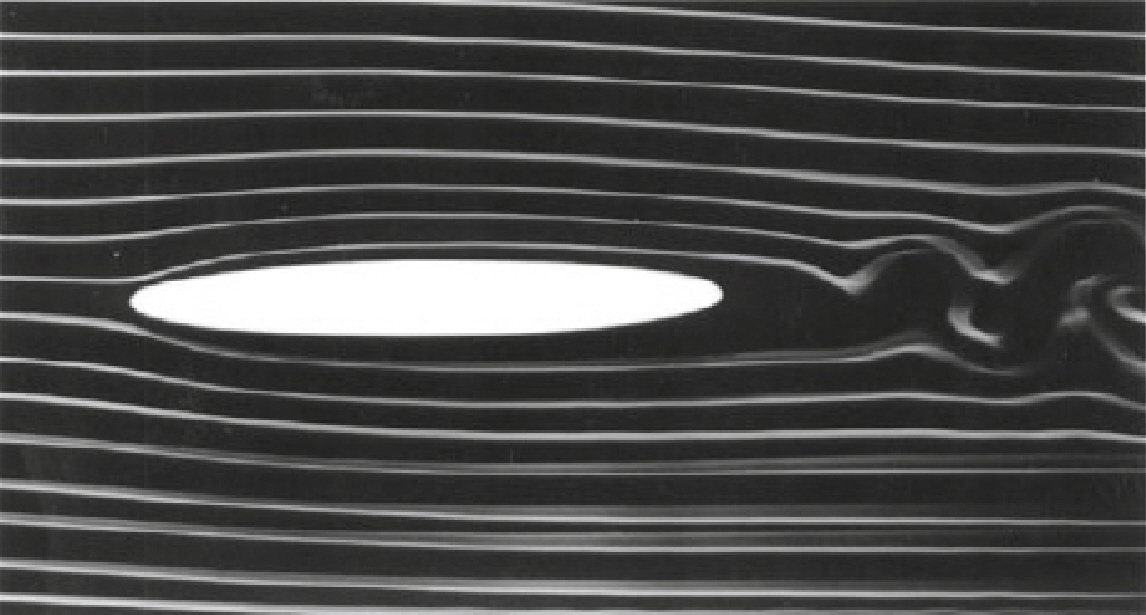
\includegraphics[width=1\textwidth]{HuchoDV013.jpg}
		\subcaption{$\sigma = 0,13$}
	\end{subfigure}
	\begin{subfigure}[c]{0.45\textwidth}
		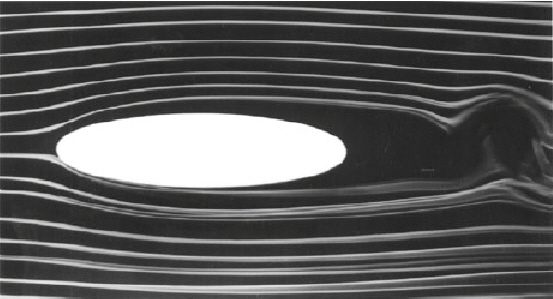
\includegraphics[width=1\textwidth]{HuchoDV026.jpg}
		\subcaption{$\sigma = 0,26$}
	\end{subfigure}
	\begin{subfigure}[c]{0.45\textwidth}
		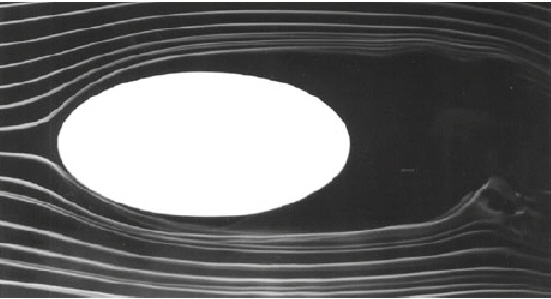
\includegraphics[width=1\textwidth]{HuchoDV05.jpg}
		\subcaption{$\sigma = 0,5$}
	\end{subfigure}
	\caption{elliptische Zylinder unterschiedlicher Dickenverh"altnisse im Rauchkanal \cite{Hucho.2011}}
	\label{fig:HuchoDV}
\end{figure}


Obwohl das Dickenverh"altnis in allgemeiner N"aherung ein gutes Ma\ss{} f"ur die Einordnung eines Stumpfk"orpers ist, zeigt sich in der Praxis, dass es nicht als notwendiges Kriterium herangezogen werden kann. So treten vergleichbare Effekte der Stumpfk"orperaerodynamik ebenfalls bei einem diskontinuierlichen Verlauf der K"orpergeometrie auf. Dies ist beispielsweise bei der ausgepr"agten Hinterkanten eines Fahrzeughecks der Fall. Der Verlauf der K"orpergeometrie muss also ebenfalls als geometrische Charakterisierung eines stumpfen K"orpers herangezogen werden.


\subsection{Str"omungsbild}
\label{sec:Stromungsbild}
Bei der Umstr"omung eines K"orpers kommt es aufgrund der Haftbedingung an dessen Kontur zur Ausbildung einer Grenzschicht. W"ahrend die Str"omungsgeschwindigkeit an der K"orperoberfl"ache Null betr"agt, passt sie sich im Grenzschichtbereich an die Anstr"omgeschwindigkeit an. Ein Teil der kinetischen Energie der Grenzschichtstr"omung wird durch Reibung an der Wand dissipiert.
Die Geometrie eines stumpfen K"orpers, wie in \abb{fig:HuchoDV} dargestellt, f"uhrt bei Umstr"omung gem"a\ss{} Bernoulli zu einer Absenkung des statischen Drucks $p$ bis zur dicksten Stelle. Hinter dieser steigt der statische Druck $p$ wieder an, wobei die durch Reibung verringerte kinetische Energie nicht mehr ausreicht, um gegen diesen anzustr"omen. Ist die kinetische Energie vollends in Druck umgewandelt, kommt es zur R"uckstr"omung, wobei die Grenzschicht abl"ost \cite{Hucho.2011}.\\
Sofern eine diskontinuierlichen Stelle in der K"orpergeometrie vorhanden ist, kann die Str"omung dieser ebenfalls nicht weiter folgen. Man spricht in diesem Fall von einem Abriss der Str"omung, welcher in der Praxis an Hinterkanten zu finden ist.

Das Abl"osen oder Abrei\ss{}en hat die Ausbildung eines Totwassers zur Folge, in dessen Gebiet sich das Fluid bedingt durch Z"ahigkeitseffekte verwirbelt und Wirbelschichten ausbildet. Dies f"uhrt zu einer Druckabsenkung hinter dem stumpfen K"orper, sodass durch den h"oheren Staupunktdruck an der Vorderseite ein Druckgradient zu verzeichnen ist. Ein Druckwiderstand ist die Folge, welcher in Str"oumgsrichtung des Fluides wirkt. Wie man in \abb{fig:HuchoStumpf} sehen kann, ist das Totwasser ein Charakteristikum des Str"omungsbildes stumpfer K"orper. Im Vergleich dazu ist dieses Gebiet beim Str"omungsbild schlanker K"orper, wie in \abb{fig:HuchoSchlank} zu sehen, nicht vorhanden, da hier ein nahezu st"orungsfreies Abstr"omen m"oglich ist. Lediglich die Reibungseffekte innerhalb der Grenzschichtstr"omung sorgen hier f"ur einen Reibungswiderstand. Schluss folglich wird der Gesamtwiderstand bei stumpfen K"orpern vom Druckwiderstand, der bei schlanken K"orpern jedoch vom Reibungswiderstand dominiert.

\begin{figure}[h]
	\centering
	\includegraphics[width=0.5\textwidth]{HuchoschlankerKorper.jpg}
	\caption{Stromlinienbild eines schlanken K"orpers im Rauchkanal \cite{Hucho.2011}}
	\label{fig:HuchoSchlank}
\end{figure}

\begin{figure}[h]
	\centering
	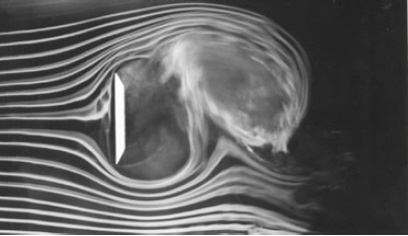
\includegraphics[width=0.5\textwidth]{HuchoStumpferKorper.jpg}
	\caption{Stromlinienbild eines stumpfen K"orpers im Rauchkanal \cite{Hucho.2011}}
	\label{fig:HuchoStumpf}
\end{figure}


Hieraus wird die Notwendigkeit ersichtlich, eine Druckerh"ohung in diesem Totwasser vorzunehmen, um den Druckgadienten und damit den Druckwiderstand zu verringern. F"ur das bessere Verst"andnis soll im nachfolgenden das Totwasser weiter spezifiziert werden.

\subsection{Totwasser}
\label{sec:Totwasser}

Wie bereits oben erw"ahnt bilden sich innerhalb des Totwassers Wirbelschichten aus. Diese entstehen bei der turbulenten Durchmischung der ehemaligen Grenzschichtstr"omung, welche nun als Scherschichtstr"omung bezeichnet wird, mit dem ruhenden Fluid im Windschatten des K"orpers. 



 
Innerhalb des Totwassers existiert eine instation"are periodische Str"omung, welche durch Druckschwankungen zu oszillierende Abl"osungen f"uhrt. Diese Oszillation wei\ss{}t eine charakteristische Frequenz auf und wird durch die Stouhal-Zahl ${Sr}$ beschrieben. 

Die Wirbel innerhalb der turbulenten Str"omung  zerfallen kaskadenartig in kleinere Wirbel und dissipieren dabei ihre Energie in W"arme, bis sie sich g"anzlich aufl"osen und sich erneut ein laminares Str"omungsprofil ausbildet. Dennoch ergibt sich im Nachlauf des stumpfen K"orpers eine Delle im Geschwindigkeitsfeld. 

\begin{figure}[h]
	\centering
	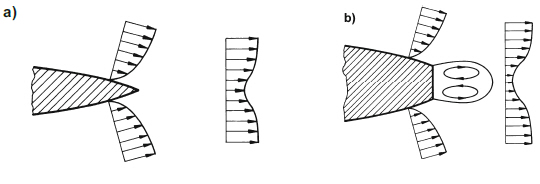
\includegraphics[width=0.7\textwidth]{Nachlauf.jpg}
	\caption{Nachlauf eines a) schlanken K"orpers und eines b) stumpfen K"orpers \cite{Hucho.2011}}
	\label{fig:Nachlauf}
\end{figure}

\subsection{Praktische Bedeutung der Stumpfk"orper}
tbd


\section{Coand\^{a}-Effekt (TG)}
%	Umströmung gekrümmter Flächen
%	Haftbedingung
%	Typische Strömungsbilder
%	technische Anwendung 

Der Coand\^{a}-Effekt tritt auf, wenn ein Strahl entlang einer konvexen K"orperkontur str"omt. Anders als die bisher betrachtete Str"omung, kann die sogenannte Coand\^{a}-Str"omung des Strahles der Kontur einer konvexen Rundung folgen ohne abzul"osen, wie dies in \abb{fig:coanda} deutlich wird. Dem Gegen"uber f"uhrt die konvexe Rundung bei einer normalen Anstr"omung nach Bernoulli zu einer Verlangsamung der Str"omung und demgem"a\ss{} einer Druckerh"ohung, was eine R"uckstr"omung und Abl"osung zur Folge hat. Dies wurde bereits in \ref{sec:Stromungsbild} diskutiert.

\begin{figure}[h]
	\centering
	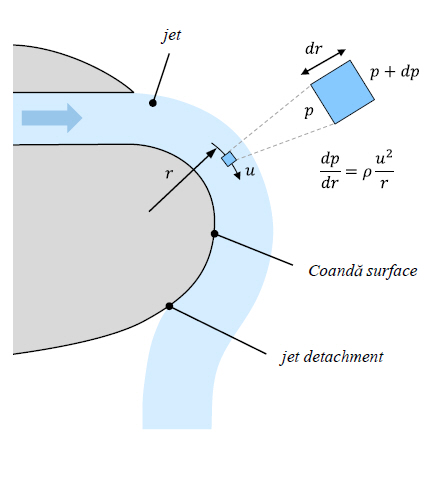
\includegraphics[width=0.5\textwidth]{coanda.jpg}
	\caption{Skizze zum Coand\^{a}-Effekt \cite{Stadlberger.2016}}
	\label{fig:coanda}
\end{figure}

Tritt ein Freistrahl in ein ruhendes Fluid ein, rei\ss{}t er an dessen R"andern das umgebende Medium mit. Um die Kontinuit"atsbedingung zu erf"ullen, entsteht am Au\ss{}enraum des Strahls eine Str"omung zur Strahlmitte, was als Entrainment-Effekt bezeichnet wird. In der N"ahe einer K"orperkontur wird das Nachstr"omen des Mediums unterbunden wird. In der Folge entsteht an der Wand ein lokaler Unterdruck und somit ein Druckgradient $dp$ quer zur Str"omungsrichtung. Dies f"uhrt zu einer Umlenkung des Freistahl in Richtung der Wand, wie in \abb{fig:coanda} ersichtlich ist. In der Folge entsteht ein Wandstrahl, welcher sich an die K"orperkontur anschmiegt \cite{Fernholz.1966}. 

Die Kr"ummung pr"agt dem Strahl eine Zentrifugalkraft auf, welche im Gleichgewicht mit der Resultierenden infolge des Druckgradienten $dp$ steht. Eine Erh"ohung der Wandkr"ummung ruft jedoch eine st"arkere Zentrifugalkraft hervor. Deshalb kann der Wandstrahl starken Kr"ummungen durch kleine Wandradien nicht folgen und l"ost ebenfalls ab \cite{Riedel.1971}

%Ausführung Riedel ergänzen
Da es sich bei der Coand\^{a}-Str"omung um einen Wandstrahl handelt, gibt es zur Grenzschicht eine zus"atzliche Reibungsschicht zum umgebenden Medium. Somit bildet sich ein Geschwindigkeitsprofil wie in \textbf{Abbildung 6 einf"ugen!} aus. \\
Im zeitlichen Mittel ist die resultierende Zentrifugalkraft proportional zu $\frac{u^2}{r+y}$. Dabei ist die wirkende Zentrifugalkraft in der N"ahe des Maximums des Geschwindigkeitsprofils des Wandstrahls proportional zu $\frac{U^2}{r+\frac{H}{4}}$. Sie ist somit aufgrund der h"oheren Geschwindigkeit gr"o\ss{}er als die Zentrifugalkraft auf Teilchen in der N"ahe der Strahloberfl"ache und in der N"ahe der K"orperkontur.\\
An der K"orperkontur ist die resultierende Zentrifugalkraft proportional zu $\frac{u^2}{r}$, an der Strahloberfl"ache jedoch nur zu $\frac{0,25 \cdot U^2}{r + H}$. Aus diesem Grund besteht die Tendenz von Teilchen in der N"ahe der Maximalgeschwindigkeit, zum "au\ss{}eren Rand und somit in das Gebiet der Strahlvermischung mit dem Umgebungsmedium abzudriften. Durch ihre geringere Zentrifugalkraft blockieren die Teilchen innerhalb des "au\ss{}eren Randes jedoch die nach au\ss{}en dringenden Teilchen und somit eine nach au\ss{}en gerichtete Bewegung. Infolgedessen treffen zus"atzliche Teilchen am Rand aufeinander, was feine Strahlvermischung bef"ordert.\\
Ein entgegengesetztes Verhalten findet sich in der N"ahe der K"orperkontur. Den Teilchen in Wandn"ahe wird eine kleinere Zentrifugalkraft als im Strahlzentrum aufgepr"agt. Weniger Kollisionen und somit eine geringere gegenseitige Beeinflussung benachbarter Teilchen sind die Folge. Dies reduziert den Turbulenzgrad verglichen mit einer ebenen Strahlstr"omung.
Stromabw"arts weitet sich die Mischbewegung vom Strahlrand zum Strahlkern und zur konturnahen Str"omung aus, weshalb der Turbulenzgrad infolge der Strahlvermischung steigt \cite{Riedel.1973}. 

Wie bereits oben erw"ahnt wurde, wird am freien Rand das umgebende Fluid mitgerissen, was gleichzeitig zu einer Reduktion der kinetischen Energie des Strahls f"uhrt. Die daraus resultierende Verlangsamung der Coand\^{a}-Str"omung sorgt daf"ur, dass die Abl"oseneigung des Strahls mit der Laufl"ange zunimmt \cite{Fischer.2011}. Aus dieser Beobachtung heraus wurde der Anlegewinkel f"ur Coand\^{a}-Str"omung an einem Zylinder durch Newman definiert \cite{Newman.1961}. Dieser beschreibt das Verh"altnis vom Radius $R$ der konvexen K"orperkontur zur Ausdehnung $h$ des Strahls. Die Ausdehnung $h$ des Strahls wird durch die Spalth"ohe bestimmt, weshalb der Anlegewinkel eine fundamentale Beziehung geometrisch signifikanter Gr"o\ss{}en der Coand\^{a}-Fl"achen-Ausblasung beschreibt. Infolge h"oherer Zentrifugalkr"afte bei gro\ss{}en Wandkr"ummungen nimmt der Anlegewinkel bei kleinen $\frac{h}{R}$ und konstanten Ausblasimpuls zu. Wird die Spalth"ohe kleiner, erh"oht sich gem"a\ss{} der Kontinuit"atsgleichung die Ausblasgeschwindigkeit. Diese Geschwindigkeiterh"ohung sorgt f"ur eine Effektivierung des Entrainment-Effektes und in Folge dessen ebenfalls der Coand\^{a}-Effekt \cite{Fischer.2011}.


%%
%Da es sich bei der Coand\^{a}-Str"omung um einen Wandstrahl handelt, gibt es zur Grenzschicht eine zus"atzliche Reibungsschicht zum umgebenden Medium. Dies wird in \abb{fig:coanda} gezeigt. Da das Umgebungsmedium ruht, gibt es gem"a\ss{} Bernoulli keinen Druckanstieg entlang der konvexen Rundung, die Grenzschicht bleibt stabil. Aus diesem Grund haftet die Coand\^{a}-Str"omung l"anger an K"orperkontur an.




%%%%%%%%%%%%%%%%%%%%%%%%%%%%%%%%NORAS REICH ;) %%%%%%%%%%%%%%%%%%%%%%%%%%%%%%%%%%%%%%%%%%%%%%%%%
\newpage
\section{Aktive Str\"omungsbeeinflussung (NB)}

Stumpfe K"orper haben meist ein stufenartiges Ende, an dem sich str"omungsmechanische Nachteile ergeben. Deshalb soll durch eine Anpassung der Geometrie des K"orpers oder durch die strukturelle Ver"anderung des Todwassers dieser ausgeglichen werden. Ziel ist es, den Basisdruck anzuheben und dar"uber den Druckwiderstand des K"orpers zu verringern \cite{Hucho.2011}.\\
%hier evtl ein paar passive verfahren
Die nachfolgende Arbeit konzentriert sich auf ein aktives Verfahren der Str"omungsbeeinflussung, weshalb im folgenden einige bis jetzt realisierte Verfahren vorgestellt werden.\\

%-------------------------------------------------------------------------------------
Bearman \cite{Hucho.2011} hat als einer der ersten die aktive Str"omungsbeeinflussung nachgewiesen. \abb{fig:Bearman} zeigt das verwendete Stumpfk"orpermodell. Dabei ist als Besonderheit auf die por"ose Basis \(A_{0}\) hinzuweisen, durch die zus"atzlich Luft am Ende des K"orpers ausgesto\ss{}en wird. Es werden zwei Ausblasequerschnitte \(A_{0}\) gew"ahlt, einmal "uber fast die gesamte Fl"ache und einmal "uber knapp die H"alfte der Fl"ache in der Mitte angeordnet.
\begin{figure}[h]
	\centering
	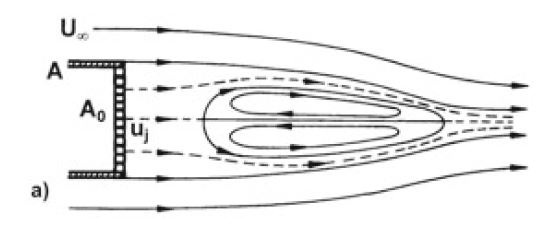
\includegraphics[width=0.5\textwidth]{KorperBearman.jpg}
	\caption{Stumpfk"orper mit Ausblasung von Bearman \cite{Hucho.2011}}
	\label{fig:Bearman}
\end{figure}\\
Der Druck hinter dem K"orper nimmt mit wachsendem Volumenstrom zu. Die austretende Luft sorgt daf"ur, dass die Str"omungsabl"osung vom K"orperende weggeschoben wird. Sie fungiert wie eine Trennplatte im Bereich der passiven Str"omungsbeeinflussung. Durch die erst weiter hinten stattfindende Verwirbelung, f"allt der Widerstand des K"orpers ab.

%-------------------------------------------------------------------------------------
Geropp und Odenthal beschreiben in \cite{Geropp.2000} Experimente zur Einblasung am Ende eines Kraftfahrzeuges "uber zwei Schlitze mit Nutzung des Coand\^{a}-Effekts (\abb{fig:Geropp}).
\begin{figure}[h]
	\centering
	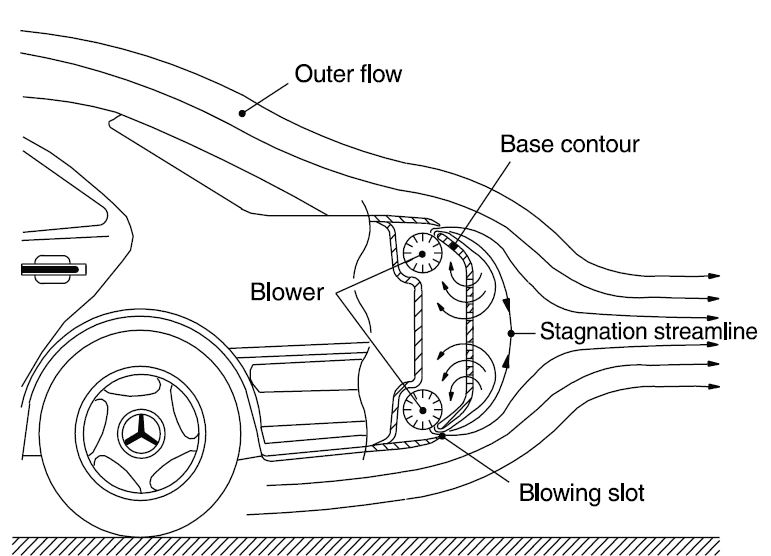
\includegraphics[width=0.5\textwidth]{KorperGeropp.jpg}
	\caption{Stumpfk"orper mit Ausblasung von Geropp \cite{Geropp.2000}}
	\label{fig:Geropp}
\end{figure}\\
Hierbei ist f"ur die Beeinflussung der Grenzschicht die Ausblasung bei hohen Geschwindigkeiten erforderlich. Durch den Coand\^{a}-Effekt wird die eingeblasene Luft in das Todwasser umgelenkt, wo sie wieder abgesaugt wird. Dadurch wird der Druck hinter dem Fahrzeug erh"oht und der Gesamtwiderstand verrringert. Die Experimente zeigen, dass eine Druckerh"ohung von~50\% und eine Widerstandsverringerung um 10\% m"oglich ist. Au\ss{}erdem wird ein Energievorteil f"ur moderate Ausblasgeschwindigkeiten mathematisch festgestellt.

%--------------------------------------------------------------------------------------
In \cite{Barros.2016} wird zus"atzlich zu den vorher beschriebenen Verfahren die Ausblassung gepulst durchgef"uhrt. Dabei soll der Einfluss von Frequenz und Amplitude auf das Widerstandsverhalten untersucht werden.\\
In \abb{fig:Barros} ist der schematische Aufbau der gepulsten Ausblasung dargestellt. Diese wird "uber Ventile realisiert, die eine Rechteckkurve mit einem duty cycle (weitere Erl"auterungen in \kap{s:rotierendeWalzen}) von 40\% erzeugen. Direkt unter der Ausblasstelle wird zus"atzlich noch eine Coand\^{a}-Fl"ache befestigt.\\
\begin{figure}[h]
	\centering
	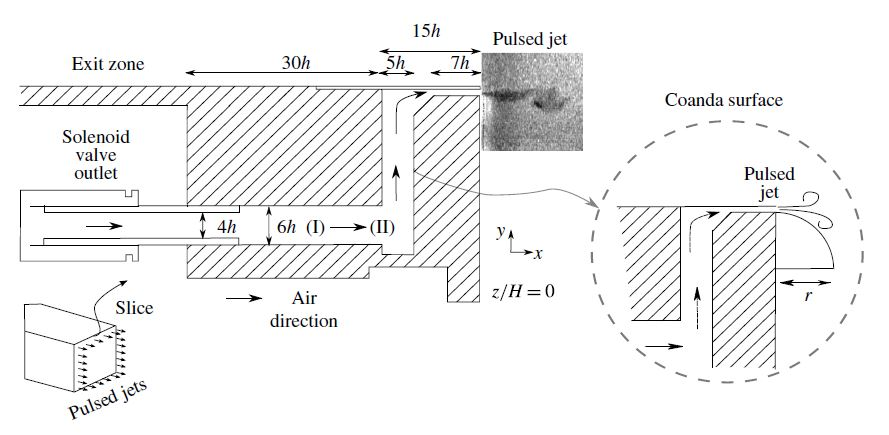
\includegraphics[width=0.7\textwidth]{KorperBarros.jpg}
	\caption{Ausblasung von \cite{Barros.2016}}
	\label{fig:Barros}
\end{figure}
Mit eher steigender Frequenz und steigender Amplitude, wurde eine Umlenkung der Grenzschicht beobachtet. "Uber eine gepulste Einblasung, nahe der nat"urlichen Abl"osefrequenz der Str"omung, kann nach \cite{Barros.2016} der Widerstand am meisten (10\%) gesenkt werden. Bei zus"atzlicher Nutzung der Coand\^{a}-Fl"ache kann eine Reduktion von 20\% erreicht werden.

%-------------------------------------------------------------------------------------
Modi et al. \cite{MODI.1991} versucht durch drehende Zylinder den Widerstand zu reduzieren. Dabei benutzt \cite{MODI.1991} unterschiedliche Modelle. F"ur erste Versuche wird das Modell in \abb{fig:Modi3} benutzt und sp"ater der Truck aus \abb{fig:Modi}.
\begin{figure}[h]
	\centering
	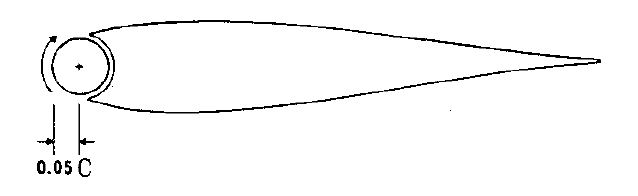
\includegraphics[width=0.6\textwidth]{KoerperModi3.jpg}
	\caption{Stumpfk"orpermodell mit Walze von Modi et al. \cite{MODI.1991}}
	\label{fig:Modi3}
\end{figure}\\
F"ur den K"orper in \abb{fig:Modi3} sind Str"omungsbilder (\abb{fig:ModiStr}) aufgenommen worden. Diese sind mit einem Anstellwinkel des K"orpers von 20 Grad entstanden. Das Verh"altnis der Drehgeschwindigkeit der Zylinder \(U_c\) bzgl. der Anstr"omgeschwindigkeit \(U\) wurde variiert.\\
\begin{figure}[h]
	\centering
	\begin{subfigure}[c]{0.4\textwidth}		
		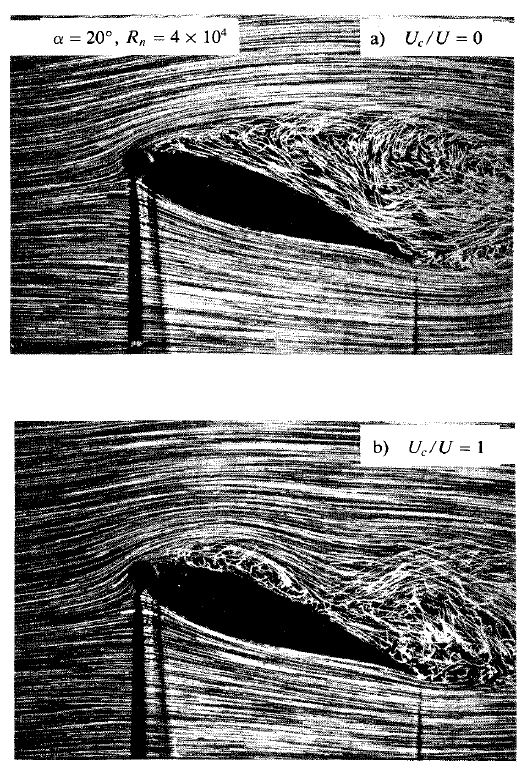
\includegraphics[width=0.7\textwidth]{ModiStr1.jpg}
	\end{subfigure}
	\begin{subfigure}[c]{0.4\textwidth}
		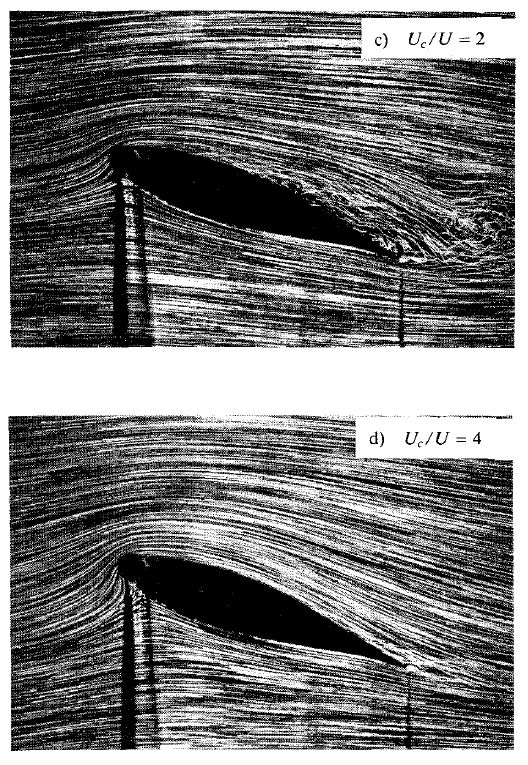
\includegraphics[width=0.7\textwidth]{ModiStr2.jpg}
	\end{subfigure}
	\caption{Str"omungsbilder von Modi et al. \cite{MODI.1991}}
	\label{fig:ModiStr}
\end{figure}

Auf den Str"omungsbildern (\abb{fig:ModiStr}) kann gut gesehen werden, dass bei nicht rotierenden Zylindern \(U_c/U=0\) (oben links) die Abl"osung stark ist im Vergleich zu \(U_c/U=4\) (unten rechts), hier drehen die Zylinder viermal schneller als die Anstr"omung.\\
\begin{figure}[h]
	\centering
	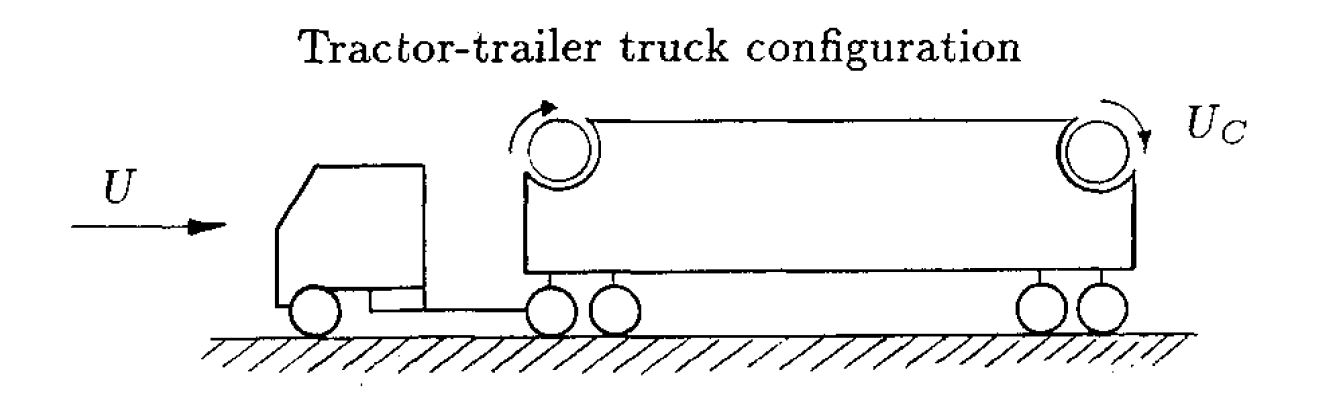
\includegraphics[width=0.6\textwidth]{KorperModi.jpg}
	\caption{Erstes Truckmodell von Modi et al. \cite{MODI.1991}}
	\label{fig:Modi}
\end{figure}
Bei den Versuchen am Truckmodell sind die Zylinder zuerst angeordnet, wie in \abb{fig:Modi} dargestellt. Bei dem ersten Versuch werden die Rauhigkeiten der Zylinder variiert. Es gibt einen glatten Zylinder, einen mit einer Rauhigkeit von 40 und einen mit 80. Au\ss{}erdem wird wieder das Verh"altnis der Drehgeschwindigkeiten der Zylinder \(U_c\) bzgl. der Anstr"omgeschwindigkeit \(U\) f"ur alle drei F"alle variiert. Daraus ergeben sich die Widerstandsreduktionen in \tab{tab:Modi}.\\
\begin{table}[h]
	\centering
	\begin{tabular}{lrr}
		\toprule
		Zylinder & Widerstandsreduktion [\%] & \(U_c/U\)\\
		\midrule
		glatt & 5 & 2\\
		Rauhigkeit 80 & 10 & 2.1\\
		Rauhigkeit 40 & 13 & 2.1\\
		\bottomrule
	\end{tabular}
	\caption{Widerstandsreduktion bei Modi}
	\label{tab:Modi}
\end{table}
Da der hintere Zylinder keinen Impuls in die Grenzschicht einbringen kann, wurde ein zweites Experiment mit anderer Konfiguration durchgef"uhrt. Dabei wurde ein Zylinder mit spiralf"ormiger Rille in der Oberfl"ache und einer mit einer Vielkeil-Verzahnung, deren Rillen parallel zur Drehachse verlaufen, verwendet. Die Position des ersten Zylinders bleibt unver"andert, der Zweite wird ans Ende des ersten Drittels der Truckoberseite positioniert (siehe \abb{fig:Modi2}).\\
\begin{figure}[h]
	\centering
	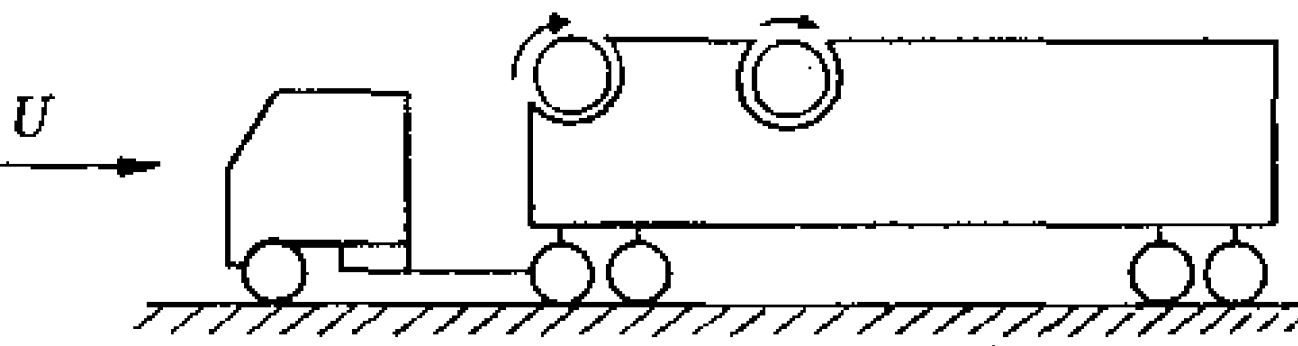
\includegraphics[width=0.5\textwidth]{KoerperModi2.jpg}
	\caption{Zweites Truckmodell von Modi et al. \cite{MODI.1991}}
	\label{fig:Modi2}
\end{figure}\\
Der spiralf"ormige Zylinder erzielte das gleiche Ergebnis, wie der Zylinder mit einer Rauhigkeit von~40 im ersten Experiment. Der Vielkeil-Verzahnungszylinder hat allerdings einen gro\ss{}en Einfluss auf den Widerstand. Bei alleiniger Betrachtung des vorderen Zylinders wird eine Reduktion von~29\% erreicht, beide Zylinder erreichen bis zu 41\%.

%------------------------------------------------------------------------------------
In \cite{Gong.2015} wird eine r"uckwertsgewandte Stufe ein 2D-Modell und anschlie\ss{}end ein 3D-Model (\abb{fig:Gong}) untersucht. Das besondere dabei ist die Anregungsform "uber einen Lautsprecher, der ein monofrequentes, sinusf"ormiges Anregunfgssignal durch kleine L"ocher in die Str"omung gibt. "Uber die Sinusfunktion wird erreicht, dass die eingestr"omte Masse "uber eine Periode betrachtet gleich Null ist. Neben der Untersuchung im Windkanal wurde eine instation"are Simulation entwickelt und validiert, diese Erm"oglicht einen genaueren Einblick in die Wirbelstrukturen.
\begin{figure}[h]
	\centering
	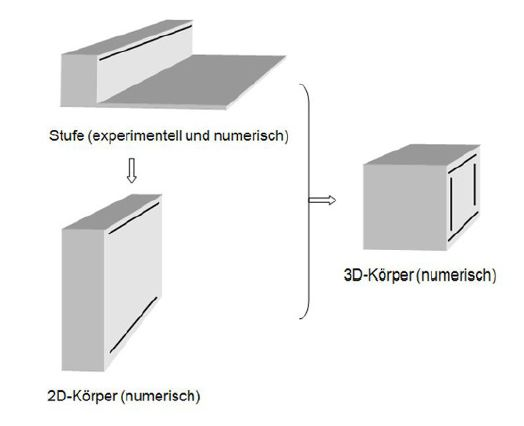
\includegraphics[width=0.5\textwidth]{KoerperGong.jpg}
	\caption{Modelle nach Gong \cite{Gong.2015}}
	\label{fig:Gong}
\end{figure}\\
Bei einer hochfrequenten Anregung kann die Bildung von Wirbeln unterdr"uckt werden. Dadurch wird der Druck hinter der Basis erh"oht und der Luftwiderstand des K"orpers sinkt.

%------------------------------------------------------------------------------------
Alle bisher vorgestellten Verfahren haben nur eine Steuerung des Vorgangs betrachtet. In \cite{Henning.2008} wird jetzt zus"atzlich eine Regelung des Mechanismuses der Str"omungsbeeinflussung eingef"uhrt. Dabei m"ochte man "au\ss{}ere St"orungen mit ber"ucksichtigen, die zum Beispiel sich gegenseitig beeinflussende Kraftfahrzeuge aufeinander haben.\\
Im Rahmen der Arbeit \cite{Henning.2008} wurden unterschiedliche K"orper "ahnlich zu denen in \abb{fig:Gong} analysiert.
%\begin{figure}[h]
%	\centering
%	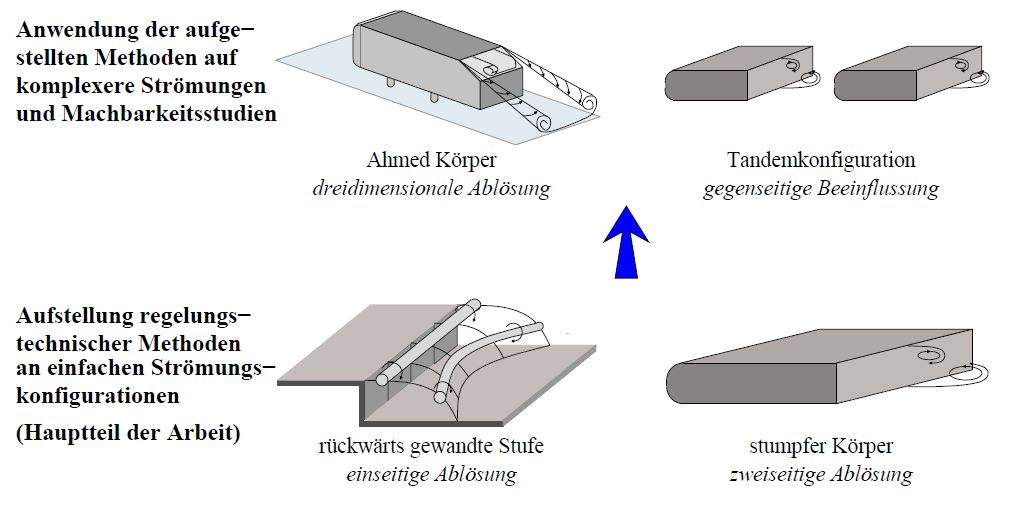
\includegraphics[width=0.8\textwidth]{KorperHenning.jpg}
%	\caption{betrachtete Modelle f"ur Auslegung der Regelung \cite{Henning.2008}}
%	\label{fig:Henning}
%\end{figure}\\
An der r"uck"arts gewandten Stufe wurde erfolgreich die Wideranlegel"ange "uber einen segmentierten Schlitz an der Stufenkante geregelt. Au\ss{}erdem konnte eine Unterdr"uckung von St"orungen erreicht werden. Das Ganze wurde "uber eine Robuste Regelung realisiert.\\
Am stumpfen K"orper wurde mit Hilfe einer Phasenregelung an Ober- und Unterseite eine Widerstandsreduzierung von bis zu 15\% erreicht.\\
Die Tandemkonfiguration (zwei K"orper hintereinander) wurde im Rahmen einer Machbarkeitsstudie \cite{Henning.2008} untersucht und f"ur zuk"unftige Arbeiten als sinnvoll betrachtet. Dabei geht es um die St"oreinfl"usse, die der erste K"orper auf den zweiten hat und wie dieser die St"orung "uber eine Regelung beseitigen kann, sodass auch beim zweiten K"orper eine Widerstandsreduzierung m"oglich ist.\\
Die Regelung stellt einen weiteren Schritt in Bezug auf eine Widerstandsreduktion von Stumpfk"orpern dar. Im Rahmen dieser Arbeit wird eine Regelung nicht mit betrachtet, da erst das neue Konzept untersucht werde muss. Dieses kann dann evtl. in Zukunft um eine Regelung erweitert werden.

\chapter{Konstruktion der rotierenden Walzen (NB)}
\label{s:rotierendeWalzen}
Bevor das Experiment im Windkanal stattfinden kann, m"ussen die rotierenden Walzen f"ur den Stumpfk"orper konstruiert werden. Die Walzen sitzen am Ende des K"orpers, wie in \abb{fig:modelschema} gezeigt. Es sind drei unterschiedliche Walzenpaare entstanden: ein glattes Walzenpaar, ein gezahntes Walzenpaar mit einem duty cycle von 33\% und ein gezahntes Walzenpaar mit einem duty cycle von 50 \%.\\
%Die rotierenden Walzen sind jeweils auf einer Welle gelagert und werden von Elektromotoren angetrieben. Die Elektromotoren haben eine maximale Drehrate von 3650 Umdrehungenpro Minute und eine minimale Drehrate von um die 100 Umdrehungen pro Minute.

\begin{figure}[h]
	\centering
	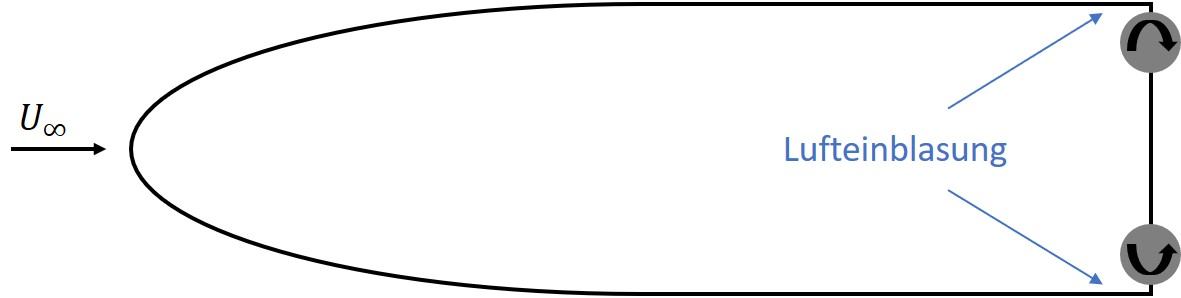
\includegraphics[width=0.8\textwidth]{ModellSchema.jpg}
	\caption{schematische Darstellung des Versuchsmodells}
	\label{fig:modelschema}
\end{figure}
Die rotierenden Walzen erf"ullen die Aufgabe der gepulsten Einblasung in die Str"omung am Ende des Stumpfk"orpers.\\
Die Walzen bestehen aus einer Aluminium Innenewelle und einem mit Presspassung verbundenen Teflonrohr. In dem Teflonrohr ist die entscheidende Zahngeometire eingebracht. F"ur die Konstruktion des Teflonrohrs mussten folgende Aspekte betrachtet werden:
\begin{enumerate}
	\item Zahnform 
	\item Anzahl der Z"ahne
	\item Zahn"offnung 
\end{enumerate}

%----------------------------------------------------------------------------------
\section{Zahnform}
F"ur die Wahl einer Zahnform muss erst das auf die Str"omung aufgebrachte Signal festgelegt werden. Als Signale kommen daf"ur unterschiedliche Funktionen in Frage: Sinus-Funktion, Dirac-Impuls, Heaviside-Funktion usw..\\
%Die Zahnform hat Auswirkungen auf das gepulste Signal, das in die Str"omung eingef"uhrt wird. Als Grundlagen f"ur die Signalform wurden folgende mathematische Funktionen (\abb{fig:function}) betrachtet.\\
%\begin{figure}[h]
%	\centering
%	\begin{subfigure}[c]{0.5\textwidth}		
%		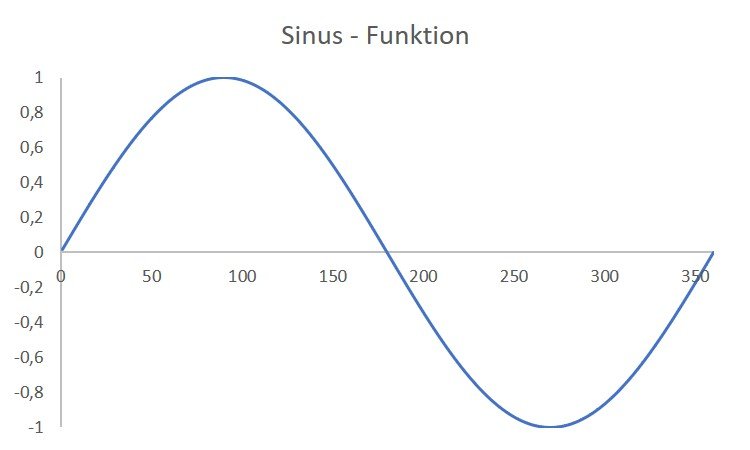
\includegraphics[width=1\textwidth]{Sinus.jpg}
%	\begin{subfigure}[c]{0.5\textwidth}
%		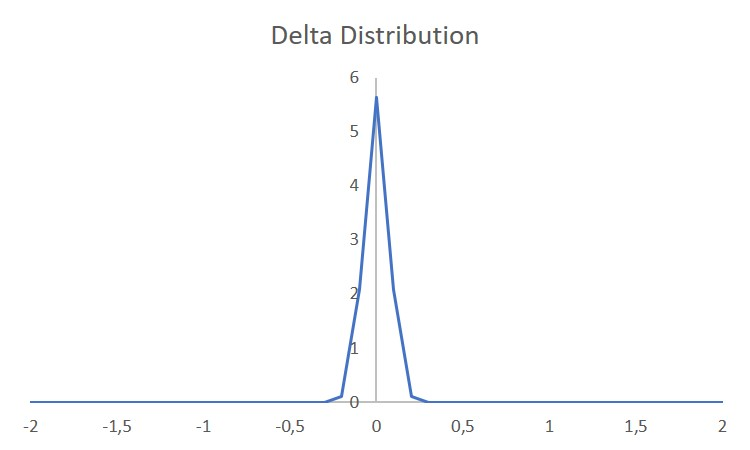
\includegraphics[width=1\textwidth]{DeltaDistribution.jpg}
%	\end{subfigure}
%	\begin{subfigure}[c]{0.5\textwidth}
%		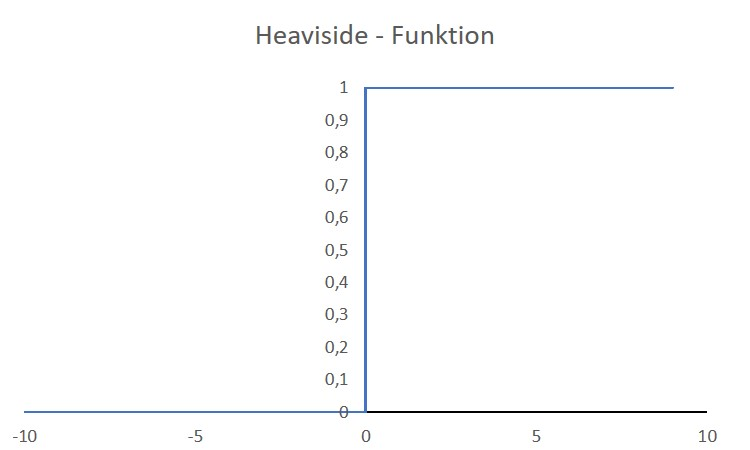
\includegraphics[width=1\textwidth]{Heaviside.jpg}
%	\end{subfigure}
%	\caption{mathematische Funktionen f"ur Zahnform}
%	\label{fig:function}
%\end{figure}\\
%F"ur die Sinus Funktion eignet sich eher eine andere Form der Str"omungsanregung, als die der drehenden Walzen. Diese kann besser "uber einen Null-Netto-Massenstrom-Jet-Aktuator \cite{Utturkar.2003} oder einen Lautsprecher dargestellt werden. Beide funktionieren "uber eine schwingende Membran, welche die Str"omung anregt.\\
%Ein Dirac-Impuls ist eine kurze Anregung der Str"omung. Die Zeit in der die Luft in die Str"omung eingeblasen wird, ist kurz im Vergleich zu der Zeit in der keine Anregung stattfindet. Damit k"onnte es zu einer nicht ausreichend gr\ss{}en Anregung kommen, die den gew"unschten Effekt nicht induziert.\\
%Eine Heaviside-Funktion stellt ein eindeutiges Signal dar, das entweder vollst"andig geschlossen oder ge"offnet ist. Somit ist eine klare Definition des Zustands m"oglich.\\
Bei der endg"ultigen Wahl eines Signals ist der fertigungstechnische Aspekt ein weiterer wichtiger Parameter, der in diesem Fall die Wahl des Signals entschieden hat. Als finales Wellendesign wurden die zwei Wellen aus \abb{fig:finalesdesign} gefertigt. Diese wurden gew"ahlt, da eine Fr"asbearbeitung des Teflonrohrs zu str"omungsmechanisch ung"unstigen Effekten gef"uhrt h"atte. Der Fr"aser hat immer eine endliche Breite, sodass die Str"omung durch die eventuell auftretenden minimalen Kanten zwischen den einzelnen Fr"asbahnen gest"ort werden k"onnte. Somit wurde sich f"ur eine Fertigung auf der Drehmaschine entschieden. Dabei wurden die Zahnt"aler "uber eine exzentrische Einspannung erreicht. Die Wahl f"ur zwei Wellen wird im Folgenden n"aher betrachtet.
\begin{figure}[h]
	\centering
	\begin{subfigure}[c]{0.4\textwidth}		
		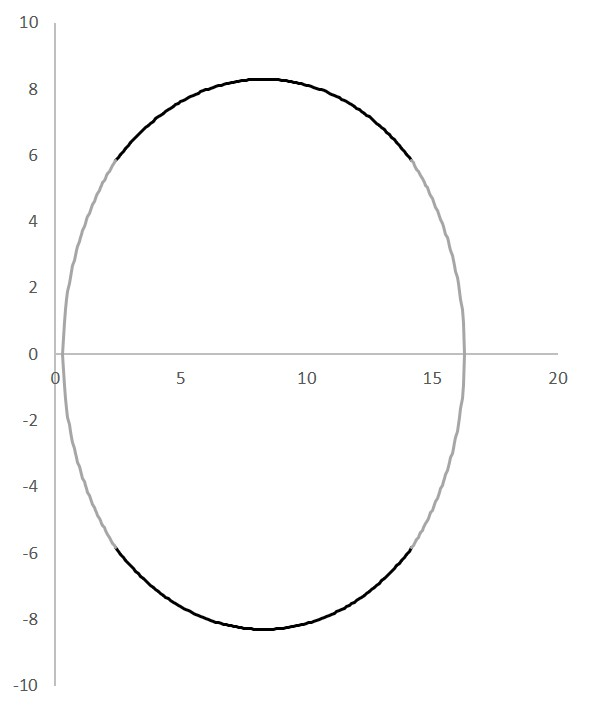
\includegraphics[width=0.8\textwidth]{Walze1Graphik.jpg}
	\end{subfigure}
	\begin{subfigure}[c]{0.4\textwidth}
		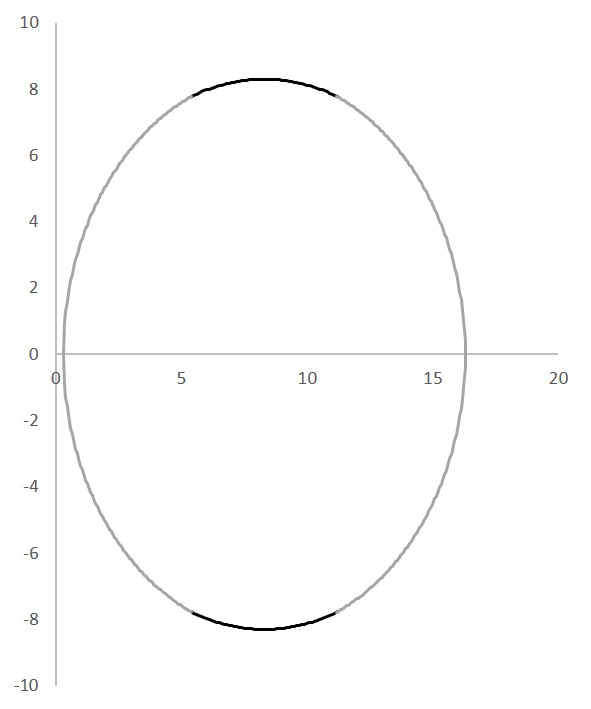
\includegraphics[width=0.8\textwidth]{Walze2Graphik.jpg}
	\end{subfigure}
	\caption{Querschnitt durch die finalen Walzen}
	\label{fig:finalesdesign}
\end{figure}\\

Die Walzenformen lassen sich "uber mehrere Kreisfunktionen auf unterschiedlichen Intervallen darstellen (verschiedene Farben in \abb{fig:finalesdesign}). Die linke Walze kann beschrieben werden "uber \glg{eq:Walze1}.
\begin{align}
	{f_1(x)}=\pm\sqrt{9,15^{2}-(x-9,45)^{2}}\,\,\,\,&x\in[0,3; 2,42] \label{eq:Walze1}\\
	{g_1(x)}=\pm\sqrt{8,3^{2}-(x-8,3)^{2}}\,\,\,\,&x\in[2,42; 14,18] \nonumber\\
	{h_1(x)}=\pm\sqrt{9,15^{2}-(x-7,15)^{2}}\,\,\,\,&x\in[14,18; 16] \nonumber
\end{align}\\
Die rechte Walze kann beschrieben werden "uber \glg{eq:Walze2}.
\begin{align}
	{f_2(x)}=\pm\sqrt{8,48^{2}-(x-8,78)^{2}}\,\,\,\,&x\in[0,3; 5,39] \label{eq:Walze2}\\
	{g_2(x)}=\pm\sqrt{8,3^{2}-(x-8,3)^{2}}\,\,\,\,&x\in[5,39; 10,61] \nonumber\\
	{h_2(x)}=\pm\sqrt{8,48^{2}-(x-7,82)^{2}}\,\,\,\,&x\in[10,61; 16] \nonumber
\end{align}\\
Aus der Form der Walzen, die die Zahnform darstellen, l"asst sich r"uckwirkend auf die Signalform schlie\ss{}en. Das Signal ist in \abb{fig:spaltverlauf} dargestellt. Ein Wert von \SI{0,3}{\milli\meter} entspricht dabei einem offenen Signal, d.h. es wird Luft in den Spalt eingeblasen. Bei einem Wert von \SI{0}{\milli\meter} findet keine Einblasung statt. In den Graphiken ist ein Signalverlauf f"ur eine Viertelumdrehung der Walze dargestellt. Aufgrund von Symmetrie folgt im weiteren ein spiegelverkehrter Verlauf und danach eine periodische Fortsetzung, wie in \abb{fig:signal} dargestellt.
\begin{figure}[h]
	\centering
	\begin{subfigure}[c]{0.7\textwidth}		
		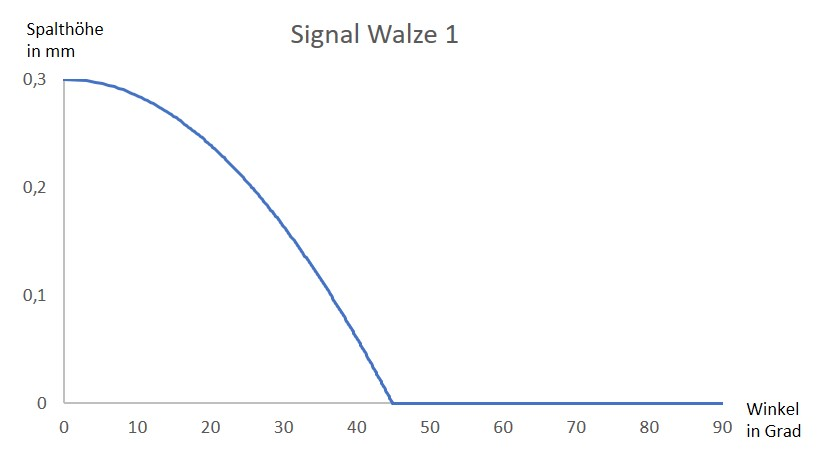
\includegraphics[width=1\textwidth]{Spaltverlauf1.jpg}
	\end{subfigure}
	\begin{subfigure}[c]{0.7\textwidth}
		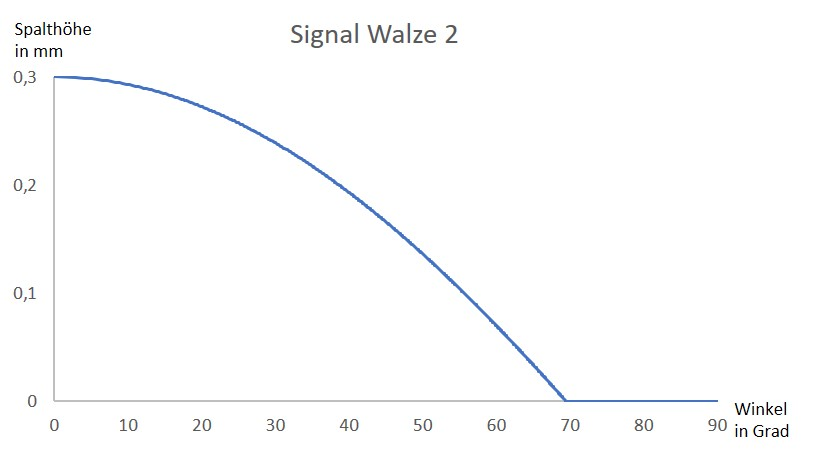
\includegraphics[width=1\textwidth]{Spaltverlauf2.jpg}
	\end{subfigure}
	\caption{Signalverlauf der Walzen}
	\label{fig:spaltverlauf}
\end{figure}

\begin{figure}[h]
	\centering
	\begin{subfigure}[c]{0.5\textwidth}		
		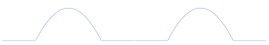
\includegraphics[width=1.2\textwidth]{SignalWalze1.jpg}
	\end{subfigure}
	\begin{subfigure}[c]{0.5\textwidth}
		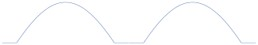
\includegraphics[width=1.2\textwidth]{SignalWalze2.jpg}
	\end{subfigure}
	\caption{Periodische Signale der Walzen}
	\label{fig:signal}
\end{figure}


%--------------------------------------------------------------------------------------
\newpage
\section{Anzahl der Z"ahne}
Als zweites wird im Folgenden auf die Entscheidung der Anzahl der Z"ahne detailierter eingegangen. Ein ausschlaggebender Punkt ist dabei, dass die Einblasung mit einer Frequenz in Umgebung der Abl"osefrequenz der Str"omung durchgef"uhrt wird. Besonders interessant ist eine Frequenz leicht oberhalb der Abl"osefrequenz (siehe \cite{Oswald.2017}). Au\ss{}erdem soll die Drehzahl der Elektromotoren nicht "uber- bzw. unterschritten werden. Diese liegt maximal bei 3650 Umdrehungen pro Minute und minimal bei 100 Umdrehungen pro Minute.\\
Die Abl"osefrequenz der Str"omung kann "uber die dimensionslose Strouhal-Zahl mit \glg{eq:Str} bestimmt werden. Wenn diese nach der gew"unschten Variable umgestellt wird (siehe \glg{eq:nachfumgestellt}) und die gegebenen Werte aus \tab{tab:Modellwerte} eingesetzt werden, kann die Frequenz
\begin{align}
	{f}=\frac{Str*U_{\infty}}{D}
		=\frac{0,23*\SI{15}{\meter\per\second}}{\SI{0,0534}{\meter}}
		=\SI{64,61}{\hertz}
		\label{eq:nachfumgestellt}
\end{align}
berechnet werden.
\begin{table}[h!]
	\centering
	\begin{tabular}{lr}
		\toprule
		Parameter & Wert\\
		\midrule
		Strouhal-Zahl & 0,23\\
		Anstr"omgeschwindigkeit & \SI{15}{\meter\per\second}\\
		Profildicke & \SI{53,4}{\milli\meter}\\
		\bottomrule
	\end{tabular}
	\caption{Modellwerte f"ur Frequenzberechnung}
	\label{tab:Modellwerte}
\end{table}\\
Aus der Frequenz, die mindestens erreicht werden soll, kann nun berechnet werden, wie schnell sich die Walze mit welcher Z"ahnezahl drehen muss. Das Ergebnis f"ur unterschiedliche Z"ahne findet sich in \tab{tab:zahnezahl}.\\
\begin{table}[h]
	\centering
	\begin{tabular}{lrr}
		\toprule
		Anzahl der Z"ahne & Drehgeschwindigkeit der Welle [Hz] & Drehgeschwindigkeit der Welle [rpm]\\
		\midrule
		1 & 64,61 & 3876,6\\
		2 & 32,30 & 1938,0\\
		4 & 16,15 & 969,0\\
		6 & 10,77 & 646,2\\
		8 & 8,08 & 484,8\\
		10 & 6,46 & 387,6\\
		\bottomrule
	\end{tabular}\\
	\caption{Z"ahnezahlen mit zugeh"origen Frequenzen}
	\label{tab:zahnezahl}
\end{table}

Aufgrund von Symmetrie und um dem m"oglichen Entstehen einer Unwucht entgegen zu wirken, wurde sich f"ur eine gerade Z"ahnezahl entschieden. Da eine ausreichend gro\ss{}e L"ucke ben"otigt wird, um den Z"ahnen einen effektiven Luftaussto\ss{} zu gew"ahrleisten, wurde sich f"ur eine Z"ahnezahl von zwei pro Walze entschieden.\\

%-----------------------------------------------------------------------------------
\section{Zahn"offnung}
Als dritten Aspekt der Zahngestaltung wird im Folgendem die Zahn"offnung betrachtet. Es wurden zwei Walzen mit zwei unterschiedlichen duty cyclen gefertigt. Die Berechnungen des duty cycles f"ur die erste Walze ist "uber Integration von \glg{eq:Walze1} und f"ur die zweite Walze von \glg{eq:Walze2} an einer Viertelwalze erfolgt. F"ur die Berechnungen wird das MATLAB Skript aus \abb{fig:Integrationsskript} verwendet. Somit ergibt sich f"ur die erste Walze ein duty cycle von 33\% und f"ur die zweite von 50\%.
\begin{figure}[h]
	\centering
	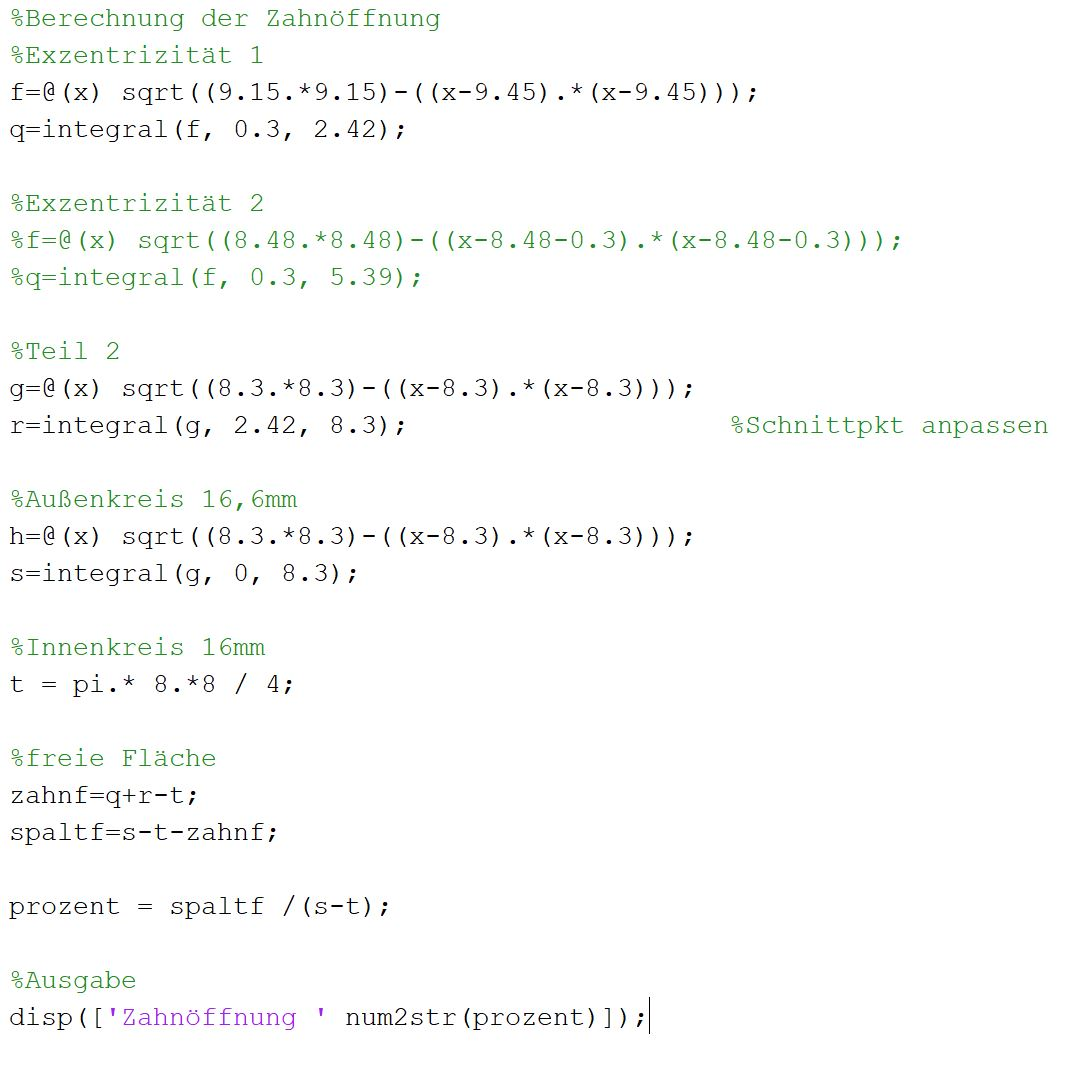
\includegraphics[width=0.8\textwidth]{Integrationsskript.jpg}
	\caption{MATLAB Skript zur Berechnung der Zahn"offnung}
	\label{fig:Integrationsskript}
\end{figure}\\




\chapter{Mathematische Vorgehensweise (FT)}\label{s:widerstandsbestimmung}

%Das Ziel dieser Arbeit ist es, festzustellen, ob die hybride aktive Str"omungsbeeinflussung von stumpfen K"orpern mittels gepulster Druckluftjets "uber zwei rotierende Coand\^{a}-Walzen mit kleiner Zahnzahl an der K"orperr"uckseite eine nennenswerte Widerstandsreduktion gegen"uber dem Fall ohne Beeinflussung erzielt. 
%Dar"uber hinaus soll getestet werden, ob die periodische Aktuierung gegen"uber vorherigen Untersuchungen mit kontinuierlicher Ausblasung den Widerstand  st"arker senken kann und diese Form der Ausblasung als effizienter betrachtet werden kann.


Damit das Ziel der Arbeit erreicht werden kann, m"ussen aus den Versuchsdaten die jeweiligen Widerstandswerte des K"orpers bestimmt werden. Dar"uber hinaus ist es erforderlich, abzusch"atzen, ob die gew"ahlte Form der Str"omungsmodifikation unter dem Schlussstrich Energie einsparen kann, oder, ob f"ur die Aktuationsmechanismen m"oglicherweise sogar mehr Energie aufgewandt werden muss, als an Einsparung gewonnen werden kann.\\
Zus"atzlich ist es von Interesse zu bestimmen, wie gro\ss{} der Impulsstrom ist, der durch die Aktuation in die Str"omung eingebracht wird und diesen ad"aquat zu kennzeichnen. 

Die Gleichungen f"ur diese Zwecke sollen in diesem Kapitel hergeleitet und n"aher erl"autert werden.

\section{Bestimmung des Widerstands mittels des Impulssatzes}
\label{sec:WueberImpulssatz}
%Die nachfolgenden Ausf"uhrungen orientieren sich eng an  Hucho \cite{Hucho.2011}.
Wie in \kap{s:grundlagen} beschrieben, besteht die Widerstandskraft $W$ eines K"orpers innerhalb einer Unterschallstr"omung im Wesentlichen aus den beiden Anteilen Reibungswiderstand und Druckwiderstand:
	\begin{equation}
	\label{eq:W_zusammensetzung}
	W = W_R + W_D
	\end{equation}
Bei schlanken K"orpern dominiert der Reibungswiderstand $W_R$ der aus Schubspannungen in der Grenzschicht der Geometrie resultiert. Bei stumpfen K"orpern hingegen ist in fast allen F"allen der Druckwiderstand $W_D$ f"ur den gr"o\ss{}eren Anteil verantwortlich. $W_D$ hat seinen Ursprung wie bereits erw"ahnt in einer "uber den K"orper schwankenden Druckverteilung.  

Bei der Untersuchung in dieser Arbeit sollen diese beiden Anteile im Folgenden jedoch nicht explizit auseinandergehalten bzw. separat bestimmt werden, da dies f"ur das Aufzeigen und Quantifizieren des ver"anderten Verhaltens durch aktive Str"omungskontrolle nicht notwendig ist.  Wir behandeln im Folgenden also nur die gesamte Widerstandskraft.

Der Widerstand $W$ eines stumpfen K"orpers innerhalb einer Str"omung macht sich als Impulsverlust stromabw"arts der umstr"omten Geometrie bemerkbar~\cite{Hucho.2011}. In \abb{fig:HuchoKV} sieht man diesen Sachverhalt durch die Delle im Geschwindigkeitsverlauf hinter dem K"orper veranschaulicht. %Die Auspr"agung dieser Delle wird 

Aus diesen "Uberlegungen folgt, dass die gesuchte Gr"o\ss{}e $W$ bestimmt werden kann, indem der Geschwindigkeitsverlauf der Str"omung im Nachlauf betrachtet und mittels des Impulssatzes ausgewertet wird. 

Der Widerstand des K"orpers selbst l"asst sich also finden, wenn ein Kontrollvolumen wie in \abb{fig:HuchoKV} um den K"orper gelegt und eine Impulsbilanz aufgestellt wird~\cite{Hucho.2011}. Es wird im Folgenden vereinfacht von einer horizontalen, inkompressiblen 2D-Str"omung ausgegangen und der Impulssatz in x-Richtung

\begin{equation}
	\label{eq:impulssatz_allg}
	\rho \int_{(K)} u_x \, \mathrm{d}Q = F_{Kx} + F_{Px} + F_{Sx}
\end{equation}
betrachtet.

Die Dichte der umstr"omenden Luft wird hierbei mit $\rho$ und die x-Komponente des Geschwindigkeitsvektors mit $u_x$ und der "uber die Kontrollfl"ache tretende Volumenstrom mit $Q$ bezeichnet.
Zudem entspricht in \glg{eq:impulssatz_allg} $F_{Kx}$ den angreifenden Volumenkr"aften, $F_{Px}$ der am freien Teil des Volumen angreifenden Oberfl"achenkr"afte (Druckkraft) und $F_{Sx}$ der St"utzkraft.

\begin{figure}[h]
	\centering
	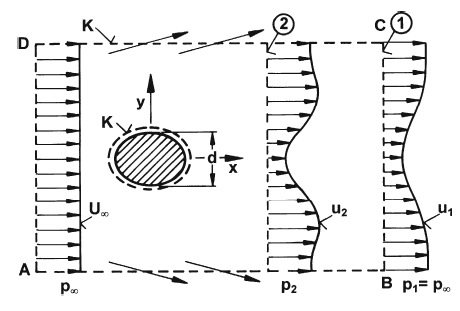
\includegraphics[width=0.6\textwidth]{KontrollvolumenHucho.png}
	\caption{Kontrollvolumen K um einen K"orper mit Geschwindigkeitsverteilungen u(x,y)~\cite{Hucho.2011}}
	\label{fig:HuchoKV}
\end{figure}

Die Volumenkraft $F_{Kx}$ kann dabei zu null gesetzt werden, da die Str"omung in Richtung x horizontal verl"auft und folglich kein Gravitationseinfluss ber"ucksichtigt werden muss. Auch abgesehen von der Gewichtskraft wirken keine anderen Volumenkr"afte.

Wenn das Kontrollvolumen, wie es in \abb{fig:HuchoKV} zu sehen ist, weit genug ab vom K"orper gelegt ist, herrscht an den Begrenzungr"andern AD, BC, AB und DC der konstante Druck $p_{\infty}$.
Dies resultiert in einer Druckkraft $F_{Px} = 0$, da sich die Kr"afte an den R"andern gegenseitig aufheben.

Infolgedessen kann die St"utzkraft nun also dem Nettoimpulsfluss gleichgesetzt werden, der
\begin{equation}
	\label{eq:nettoimpulsfluss}
	\rho \int_{(K)} \, u_x \, \mathrm{d}Q	= -\rho b \int u_1(U_{\infty} - u_1) \mathrm{d}y = F_{Sx}.	
\end{equation}
lautet.\\
Hier ist $b$ die Breite des Modells senkrecht zur Zeichenebene $u_1$ die Geschwindigkeit am Querschnitt (1) und  $U_{\infty}$ die Geschwindigkeit der umgest"orten Anstr"omung.

Die St"utzkraft des festen Teils des Kontrollvolumens - also des Stumpfk"orpers - h"angt mit dem Widerstand in der Form
\begin{equation}
	\label{eq:W=-F_Sx}
	W = - F_{Sx}
\end{equation}
zusammen.\\
$W$ ist also gleich der St"utzkraft mit negativem Vorzeichen.

Daraus folgt der Ausdruck f"ur den Widerstand zu
\begin{center}
	\begin{equation}
		\label{eq:widerstand}
		W = \rho b \int u_{1} (U_{\infty}- u_{1}) \mathrm{d}y.
	\end{equation}
\end{center}

Der Widerstand l"asst sich f"ur bessere Vergleichbarkeit dimensionslos "uber den Widerstandsbeiwert $C_w$ ausdr"ucken. Dieser ist als 
\begin{center}
	\begin{equation}
		\label{eq:def-c_w}
		C_w = \frac{W}{\frac{\rho}{2}\, U_{\infty}^2 \, bd}
	\end{equation}
\end{center}
definiert. Dabei wird der Widerstand auf die Str"omung und den charakteristischen K"orperquerschnitt $bd$ mit $d$ als H"ohe des Modells bezogen.

Nach Einsetzen der Gleichung \ref{eq:widerstand} ergibt sich f"ur den Widerstandsbeiwert
\begin{equation}
	\label{eq:Bestimmungsgleichung C_w}
	C_w = \frac{2}{U_{\infty}^2 d} \int u_{1}(U_{\infty} - u_{1}) dy.
\end{equation}
%Die Integrationsgrenzen m"ussen an die vertikale Ausdehnung der Sonden am Messrechen im Nachlauf angepasst werden.	

Um den Geschwindigkeitsverlauf zu bestimmen, k"onnen mehrere Methoden angewandt werden, wobei im Rahmen dieser Arbeit die Geschwindigkeiten aus den dynamischen Dr"ucken ermittelt werden.\\
Der Messrechen im Nachlauf liefert hierzu statische Dr"ucke und Totaldr"ucke.

Da die Wirbel an der K"orperr"uckseite periodisch abl"osen, erwarten wir am Ort der Messungen - sprich im Nachlauf - ebenfalls periodische Druckschwankungen.
Von Relevanz f"ur die zu untersuchenden Fragestellung sind dabei allerdings nur die Mittelwerte dieser Messungen "uber mehrere Perioden.
Diese werden fu"r die einzelnen Sonden in der Form
\begin{center}	
	\begin{equation}
		\overline{p}=\sum_{i=0}^{n}\frac{p_i}{n}
	\end{equation}
\end{center}
zeitlich gemittelt.
Die Summe aller "uber einen Zeitraum genommenen Dr"ucke $p_i$ wird hierbei durch die Anzahl $n$ dieser Dr"ucke innerhalb dieses Zeitraums geteilt.
Diese Mittlung gleicht zudem in gewissem Ma\ss{}e das unvermeidbare Messrauschen aus.

"Uber den die Definition des dynamischen Drucks $q$ bzw. den Zusammenhang
\begin{center}
	\begin{equation}
		\label{geschwindigkeitsformel}
		u_{1}(y)= \sqrt{\frac{2}{\rho}(p_t - p_{\infty}) } = \sqrt{\frac{2}{\rho} q(y)}
	\end{equation}
\end{center}
l"asst sich wie oben beschrieben der Geschwindigkeitsverlauf aus den gemessenen Dr"ucken bestimmen und in \glg{eq:Bestimmungsgleichung C_w} einsetzen. 

Wobei $p_t$ der Totaldruck, $p_{\infty}$ der statische Druck der freien Anstr"omung und $q$ der dynamische Druck ist.\\
Mit Hilfe dieser Formeln kann nun eine m"ogliche Reduktion des Widerstandsbeiwertes festgestellt werden.

Diese gesamte Vorgehensweise zur Bestimmung des Widerstands ist legitim, wenn an der Messstelle im Nachlauf n"aherungsweise angenommen werden kann, dass der statische Druck wieder $p_\infty$ entspricht.In diesem Fall heben sich die Druckterme im Impulssatz auf  beiden Seiten des Kontrollvolumens gegenseitig auf.
Wird die Nachlaufdelle hingegen n"aher am K"orper gemessen, weicht der dort gemessene statische Druck von $p_{\infty}$ ab.
Solche Abweichungen lassen sich durch die messtechnische Anordnung h"aufig nicht vermeiden - 
k"onnen nach \textit{B.M. Jones} aber durch eine Korrektur ber"ucksichtigt werden, wie sie beispielsweise bei \textit{Schlichting} \cite{Schlichting.2001} zu finden ist.

Hierbei werden die Dr"ucke, die theoretisch an einem Querschnitt (1) \abb{fig:HuchoKV} weit genug weg vom K"orper und somit von der statischen Druckabweichung herrschen, auf Dr"ucke zuruckgef"uhrt, die n"aher am K"orper tats"achlich gemessen werden\cite{Schlichting.2001}.
Der neue Querschnitt, bei welchem die Messung stattfindet, erh"alt den Index $(2)$.

Der Widerstand in diesem Fall ergibt sich zu
\begin{equation}
	\label{eq:widerstand_korrigiert}
	W = 2\,b \int \sqrt{p_{t2}(y) - p_2(y)} \left(\sqrt{p_{t\infty} - p_{\infty}} - \sqrt{p_{t2}(y) - p_{\infty}}\right) \mathrm{d} y_2 .
\end{equation}
Wobei $p_{t2}$ und $p_{t\infty}$ dem Totaldruck im Nachlaufquerschnitt respektive dem Totaldruck der ungest"orten Anstr"omung entspricht.

F"ur den Widerstandsbeiwert erh"alt man
\begin{equation}
	\label{eq:C_w_korrigiert}
	C_w = 2 \int_{(2)} \sqrt{\frac{p_{t2}(y) - p_2(y)}{q_{\infty}}}
	\left(1 - \sqrt{\frac{p_{t2}(y) - p_{\infty}}{q_{\infty}}}\right)  \mathrm{d}\left(\frac{y_{2}}{d}\right).
\end{equation}

Der Rechen, der die Dr"ucke liefert, sollte zu diesem Zwecke m"oglichst so platziert werden, dass die Nachlaufdelle komplett aufgenommen wird. 

Da nur diskrete Werte der jeweiligen Druckverteilung auf diese Weise ermittelt werden, m"ussen die Druckverteilungen durch eine Fitting-Funktion angen"ahert werden. 
Hierzu eignet sich - der bisherigen Erfahrung nach - der Ansatz

	\begin{equation}
	\label{eq:fitting-function}
	\frac{p(y) - p_{\infty}}{p_{min}-p_{\infty}} = (1 +ay^2)^{by^2}.
	\end{equation}
In \glg{eq:fitting-function} entspricht $p_{min}$ dem niedrigsten Druck im Nachlauf und $a$ und $b$ sind Modellparameter \cite{Oswald.2017}.

Diese Vorgehensweise hat sich beispielsweise bei einem "ahnlichem Modell durch \textit{Oswald} bew"ahrt \cite{Oswald.2017}.

Die \textit{Matlab}-Funktion \textit{nlinfit} wird hierbei genutzt, um die g"unstigsten Parameter f"ur die Druckverteilungen durch nichtlineare Regression zu bestimmen.\\
Die von \textit{nlinfit} ermittelten Druckverteilungen k"onnen dann zur Bestimmung des Widerstandsbeiwerts in \glg{eq:C_w_korrigiert} eingesetzt werden.\\
F"ur die Aufl"osung des Integrals wird die \textit{Matlab}-Funktion \textit{integral} genutzt, die globale adaptive Quadratur zur numerischen Bestimmung des Integralwerts einsetzt~\cite{Oswald.2017}.

Der vollst"andige \textit{Matlab}-Code zur Berechnung des Widerstandsbeiwerts und der Druckverteilungen ist in Anhang \ref{C_w-Code} zu finden. 

%---------------------------------------------------------------------------------------------------------------------------------------------------------------------------------
\section{Impulskoeffizient und Effizienzbetrachtung}

\subsection{Impulskoeffizient}
Der Impulskoeffizient $C_{\mu}$ wird als Ma\ss{} f"ur die Intensit"at der Ausblasung verwendet und ist im Falle von kontinuierlicher Ausblasung als 
\begin{equation}
	\label{eq: Def-momentum-coeff}
	C_{\mu} = \,\frac{\dot{m}_{jet} \cdot U_{jet}}{\frac{1}{2}\rho_{\infty}\, \cdot U^2_{\infty} \cdot A_{ref}}
\end{equation}
definiert~\cite{ElSayedM..2018}. 
Dabei entspricht $\dot{m}_{jet}$ dem Massenstrom, der durch die Spalte ausgeblasen wird. $U_{jet}$ bezeichnet die Geschwindigkeit dieses Ausblasestroms.
$A_{ref}$ wiederum dient als Bezugsfl"ache. Im Falle des getesteten Stumpfk"orpers wird als $A_{ref}$ die projizierte Fl"ache der K"orperh"ohe verwendet, da beispielsweise der Druckwiderstand einen proportionalen Zusammenhang zu dieser, f"ur stumpfe K"orper, charakteristischen Fl"ache besitzt.  %\cite{Bilges.2018}

Die Periodizit"at der Ausblasung, wie sie im Fall der zweiten Versuchskonfiguration auftritt, kann zus"atzlich im Impulskoeffizienten ber"ucksichtigt werden und f"uhrt letzendlich auf die Form \cite{Chabert.2014}
\begin{equation}
	\label{eq:momentum-coeff-oscill}
	\langle{C_{\mu}}\rangle = \frac{\rho_{jet}\langle{U^2_{jet}}\rangle \langle{A_{Spalt}}\rangle} {\frac{1}{2}\rho_{\infty}U^2_{\infty}A_{ref}}.	
\end{equation}
In \glg{eq:momentum-coeff-oscill} steht der $\langle{}\rangle$-Operator f"ur die jeweiligen zeitlichen Mittelwerte und $A_{Spalt}$ bezeichnet die Fl"ache des Ausblasespalts.

Da sowohl Plenumsdruck und somit auch die Ausblasegeschwindigkeit $U_{jet}$, als auch der Spaltquerschnitt "uber die Umdrehung der Walzen schwanken, m"ussen diese Einfl"usse wie in \glg{eq:momentum-coeff-oscill} Eingang in die Formel f"ur $C_{\mu}$ im Falle der periodischen Aktuation finden.

F"ur das mit der Zeit variierende $A_{Spalt}$   wird die mittlere Spalth"ohe, die sich von dem Zeitpunkt der "Offnung des Spalts bis zu dem Zeitpunkt, an dem der Spalt gerade wieder geschlossen ist, ermittelt.  
Durch die Betrachtung des in \kap{s:rotierendeWalzen} in \abb{fig:signal} dargestellten Spalth"ohenverlaufs ergibt sich ein $\langle{h_{Spalt,offen}}\rangle$ von ca. 0,19 \,mm.

Die mittlere Spalth"ohe "uber eine komplette Umdrehung ergibt sich durch die Multiplikation mit dem Tastgrad $\alpha$.

$U_{jet}$ muss im Falle der neu erprobten Testkonfiguration mit ovalen Wellen "uber die Plenumsdr"ucke berechnet werden.
Zun"achst werden aus den kontinuierlich ermittelten Messwerten f"ur die beiden Dr"ucke $p_{Plenum}$ mittlere Werte gebildet, die als Ausgangspunkt der Berechnung dienen.

Wir gehen weiterhin davon aus, dass der im Plenum vorhandene Druck vollst"andig in dynamischen Druck umgesetzt wird:
	\begin{equation}
	\label{eq:Annahme q}
		\langle{p_{Plenum}}\rangle = q_{jet}
	\end{equation}
In\glg{eq:Annahme q} ist $q_{jet}$ der dynamische Druck des Druckluftjets.

Da wir eine inkompressible Str"omung annehmen, kann die Geschwindigkeit $\langle{U_{jet}}\rangle$ nun als
	
	\begin{equation}
	\label{eq:jetgeschwindigkeit}
		\langle{U_{jet}}\rangle = \sqrt{\frac{2 \langle{p_{Plenum}}\rangle}{\rho_{jet}}} = \sqrt{\frac{2 \langle{p_{Plenum}}\rangle}{\rho_{\infty}}}
	\end{equation}
ausgedr"uckt werden.

Dar"uber hinaus muss wie bereits erw"ahnt der Tastgrad (\textit{engl}: duty cycle) des Signals der Walzen $\alpha$  mitbetrachtet werden.
Bei den getesteten Walzen folgt f"ur 50\,\% Tastgrad, dass die Ausblasung zumindest theoretisch exakt "uber die H"alfte einer Walzenumdrehung erfolgt.
%Daraus folgt f"ur den Impulskoeffizient mit Ber"ucksichtigung der Periodizit"at die Gleichung
%\begin{equation}
%	\label{eq:momentum-coeff-oscill-alpha}
%	\langle{C_{\mu}}\rangle = \alpha C_{\mu}
%\end{equation}	 

Wenn nun zus"atzlich bedacht wird, dass "uber zwei als gleich angen"aherte Spalte ausgeblasen wird, k"urzt sich dieser Faktor 2 genau mit dem Tastgrad und wir erhalten als modifizierten Impulskoeffizienten f"ur die zweite Testkonfiguration

	\begin{equation}
	\label{eq:momentum-coeff-oscill-final}
		\langle{C_{\mu}}\rangle = \frac{\rho_{jet}\langle{U^2_{jet}}\rangle \langle{A_{Spalt}}\rangle} {\frac{1}{2}\rho_{\infty}U^2_{\infty}A_{ref}} = \frac{2\langle{p_{Plenum}}\rangle \langle{h_{Spalt,offen}}\rangle \cdot b_{Spalt}} {\frac{1}{2}\rho_{\infty}U^2_{\infty}A_{ref}}
	\end{equation}

Mittels des Impulskoeffizienten kann die Effektivit"at der Ausblasung beschrieben werden.
Auch f"ur den Vergleich zwischen den untersuchten Walzenpaaren und mit den Daten von \textit{Bilges} \cite{Bilges.2018} ist die Betrachtung des Impulskoeffizienten ma\ss{}geblich.

\subsection{Leistungskoeffizient und Leistungsrate}
Eine alleinige Betrachtung und ein Vergleich der $C_w$-Werte f"ur den Fall ohne Druckluftzuf"uhrung und rotierende Walzen, sowie den Fall mit aktiver konstanter sowie periodischer Stro"mungsbeeinflussung ist nicht ausreichend, um eine vollst"andige Bewertung der unterschiedlichen Konfigurationen vorzunehmen.

Die durch eine Widerstandsreduktion bedingte Leistungseinsparung im Anwendungsfall k"onnte durchaus durch die extern aufzubringende Leistung f"ur Druckluft und Walzenrotation ausgeglichen oder "ubertroffen werden, sodass letztendlich zus"atzliche Energie aufgebracht und der Zweck der Anwendung verfehlt w"urde.

Ob diese Form der Str"omungsbeeinflussung also eine reale Netto-Leistungseinsparung zur Folge hat, muss folglich durch andere Kennzahlen quantifiziert werden.

Zun"achst verwenden wir f"ur die Effizienzbetrachtung eine Leistungsrate $PR$, die als 

\begin{equation}
	\label{eq:leistungsrate}
	PR = \frac{(W_0 - W)\cdot U_{\infty}}{\frac{1}{2} \dot{m_j} u_j^2 + \, P_M}
\end{equation}
eingef"uhrt wird~\cite{Freund.1994}.

Der Z"ahler dr"uckt die eingesparte Widerstandsleistung des Falls mit aktiver Str"omungsbeeinflussung im Vergleich mit dem neutralen Fall aus.
Dieser Term quantifiziert somit, in welchem Umfang die Energiedissipation in der Str"omung im zweiten Versuch reduziert wird.

Der Nenner repr"asentiert hingegen die Leistung welche dem Modell bzw. der Str"omung von externer Quelle zugef"uhrt werden muss, um den gew"unschten Effekt zu erzielen.

Der erste Summand $\frac{1}{2}\,\dot{m_j} u_j^2$ charakterisiert die kinetische Leistung der Druckluft-Jets, die durch die Spalte ausgeblasen werden. Diese Darstellung vernachl"assigt, dass die  Druckluftbeaufschlagung in den Leitungen Verluste mit sich tr"agt und auch der Kompressor selber keinen optimalen Wirkungsgrad besitzt. Somit handelt es sich bei diesem Term um die idealisierte Jet-Leistung.

Der zweite Summand $ P_M$ ist die kombinierte Motorleistung und tr"agt dem Zustand Rechnung, dass die rotierenden Walzen von zwei Elektromotoren angetrieben werden m"ussen. Diese sind f"ur den Ausgleich der an den Walzen auftretenden Widerst"anden wie Reibung an den Lagern zust"andig.
Diese Leistung wird mittels eines Leistungsmessger"ats ermittelt und manuell f"ur die Versuchsreihen notiert.

Eine negative Leistungsrate kennzeichnet F"alle in denen der Widerstand gegen"uber der Referenzmessung gestiegen ist. Eine positive Leistungsrate unterhalb von $1$ ergibt sich bei Konfigurationen, bei denen zwar der Widerstand durch die Aktuation gesenkt werden, dieser Gewinn die Kosten aber nur anteilig ausgleichen kann.\\
Erst bei Leistungsraten oberhalb von $PR = 1$ wird durch die aktiven Ma\ss{}nahmen zur Widerstandsreduzierung eine tats"achliche Leistungsersparnis generiert.

Mit \glg{eq:def-c_w} kann man die Leistungsrate auch als
\begin{equation}
	\label{eq:leistungsrate_cw}
	PR = \frac{(C_{W0} - C_W)\cdot \frac{\rho_{\infty}}{2} U^3_{\infty}\,A_{ref}}{\frac{1}{2} \dot{m_j} u_j^2 + \, P_M}
\end{equation}
schreiben.

Des Weiteren wird noch als Gr"o\ss{}e der Leistungskoeffizient $C_{Power}$ ben"otigt, welcher als
\begin{equation}
	\label{eq:def-powercoefficient}
	C_{Power,jet} = \frac{E_{jet}\dot{m}_{jet} + p_{jet}U_{jet}A_{jet} - (E_p\dot{m}_p + p_p U_p A_p)}{\frac{1}{2}\rho_{\infty}U^3_{\infty} A_{ref}}
\end{equation}

mit
\begin{equation}
	\label{eq:def-energieterm}
	E = c_vT + \frac{U^2}{2}
\end{equation}		
definiert ist~\cite{Hucho.2011}.

Gr"o\ss{}en mit Index $p$ entsprechen dabei den Gr"o\ss{}en innerhalb des Plenums, in dem die Str"omung nicht kontrahiert wird.
Des Weiteren bezeichnet $c_v$ die spezifische W"armekapazit"at von Luft bei konstantem Volumen, $T$ die Temperatur der Luft und $U$ die Geschwindigkeit.

Dieser Koeffizient dr"uckt das Verh"altnis der aufzubringenden Leistung durch die Aktuation zur in der Antsr"omung vorhandenen Leistung aus.

Im Rahmen dieser Versuche wenden wir auf \glg{eq:def-powercoefficient} einige Vereinfachungen an. 

Zun"achst treffen wir die Annahmen, dass die Temperatur innerhalb des ausgeblasenen Luftstroms gleich der Temperatur im Plenum ist
	\begin{equation}
	\label{eq:T-Vereinfachung}
		T_{jet} = T_{Plenum}
	\end{equation}
und wir n"aherungsweise davon ausgehen k"onnen, dass im Plenum keine Str"omungsgeschwindigkeit 
	\begin{equation}
	\label{eq:Up}
		U_{Plenum} \approx 0
	\end{equation}
vorliegt.

Des Weiteren nehmen wir, wie zuvor, an, dass die Str"omung inkompressibel ist und somit
	\begin{equation}
	\label{eq:Inkompressibilitaet}
		\rho_{jet} = \rho_{Plenum} = \rho_{\infty}
	\end{equation}
gilt.

Damit folgt f"ur den Leistungskoeffizienten der Ausblasung

	\begin{equation}
	\label{eq:CPowerJ vereinfacht}
		C_{Power,Jet} = \frac{\frac{1}{2}\,U^2_{jet} \cdot \dot{m}_{jet} \, + p_{jet}U_{jet}A_{jet}}{\frac{1}{2}\rho_{\infty}U^3_{\infty}A_{ref}}.
	\end{equation}

Im Falle periodischer Ausblasung muss anstatt $A_{jet}$ wieder $\langle{A_{jet}}\rangle$ verwendet werden.

Neben der Ausblasung wird auch der Aktuation durch die Walzen ein Leistungskoeffizient zugewiesen, welcher als
		\begin{equation}
		\label{eq:def-CPowerM}
			C_{Power,M} = \frac{P_M}{\frac{1}{2}\rho_{\infty}U^3_{\infty}A_{ref}}
		\end{equation}
		
definiert wird.
$P_M$ entspricht hierbei wie zuvor der kombinierten Leistung der beiden Motoren.
\chapter{Experimentelle Untersuchungen im Windkanal}
\label{s:versuche}
%%%%%%%%%%%%%%%%%%%%%%%%Modellbeschreibung Tim%%%%%%%%%%%%%%%%%%%%%%%%%%%%%
\section{Das Versuchsmodell (TG)}
Die Versuche werden am gleichen Modell duchgef"uhrt, welches im Zuge der Arbeit von Bilges \cite{Bilges.2018} verwendet wurde. Die Form entstammt der Arbeit von Oswald \cite{Oswald.2017}. Eine Skizze des Modells ist in \abb{fig:SkizzeModell} zu sehen.

\begin{figure}[h]
	\centering
	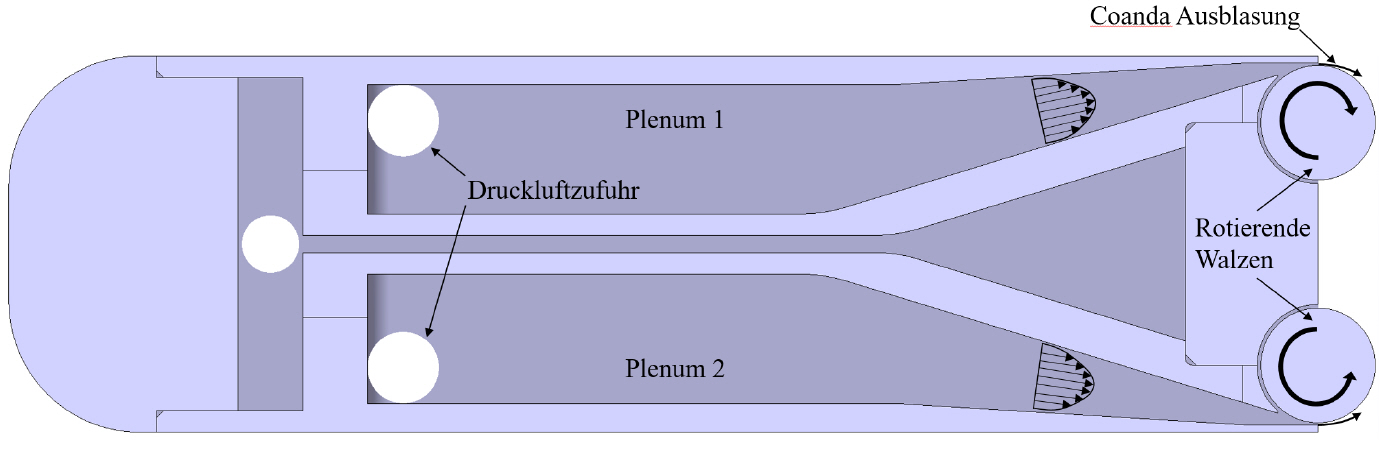
\includegraphics[width=0.9\textwidth]{SkizzeModell.jpg}
	\caption{Skizze des Versuchsmodells \citep{Bilges.2018}}
	\label{fig:SkizzeModell}
\end{figure}

Im Inneren teilt sich der Stumpfk"orper in zwei Kammern auf, welche mit Plenum 1 und Plenum 2 an der Ober- respektive Unterseite des K"orpers bezeichnet sind. "Uber die eingezeichneten "Offnungen im vorderen Teil werden die beiden Plenen "uber 4 Druckluftschl"auche mit bis zu 8 bar Druckluft versorgt, wobei diese in den Hinterteil des K"orpers str"omt. Hier findet durch den eingezeichneten Spalt eine Coanda-Ausblasung "uber die entgegengesetzt rotierenden Walzen aus Kapitel \ref{s:rotierendeWalzen} statt.

Zur Bestimmung der Oberfl"achendr"ucke sind entlang der K"orperkontur mittig an der Ober- und Unterseite 32 Druckluftbohrungen platziert worden. Die Position der Bohrungen sowie die folgend beschriebene Geometrie des K"orpers ist in \abb{fig:ModellGeometrie} ersichtlich. Das Modell kann als D-Stumpfk"orper klassifiziert werden und hat folgende Abmessungen: 
\begin{center}
H"ohe: h = 53,4 mm\\
Breite: b = 390 mm\\
L"ange: l = 190,6 mm\\ 
\end{center}
Dabei ist die Breite des Modells so gew"ahlt, dass dessen Seiten inklusive Fl"achendichtungen b"undig an der Windkanalwand abschlie\ss{}en. 

\begin{figure}[h]
	\centering
	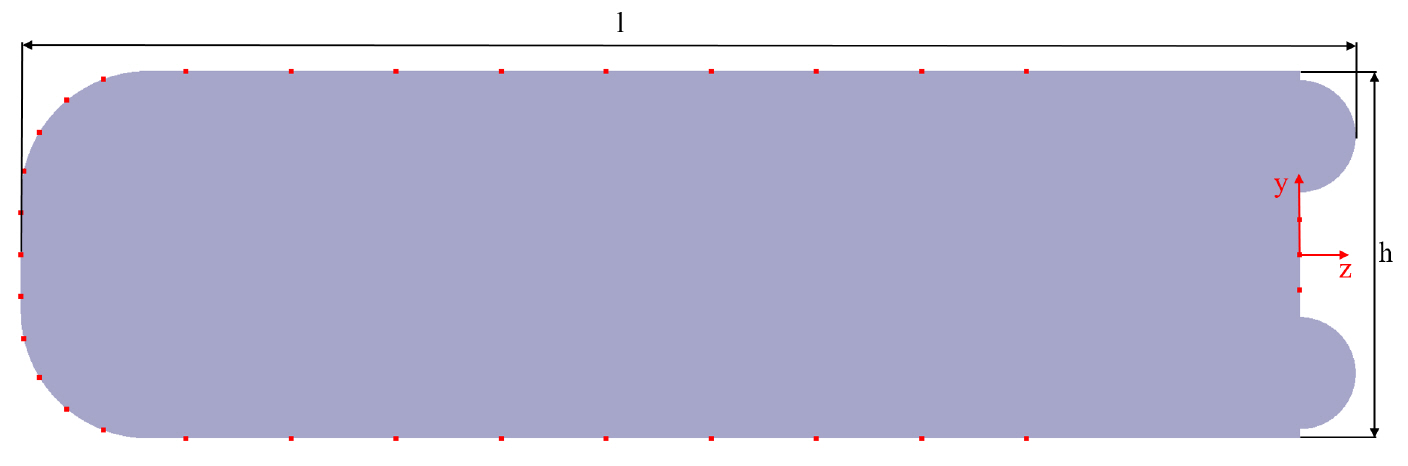
\includegraphics[width=0.9\textwidth]{ModellGeometrie.jpg}
	\caption{Geometrie des D-Stumpfk"orpers mit eingezeichneten Druckbohrungen \citep{Bilges.2018}}
	\label{fig:ModellGeometrie}
\end{figure}

Die oben erw"ahnten Druckmessbohrungen sind in \abb{fig:DModell1} erkennbar. Deren Messschl"auche werden vorne an den Seiten des Modells herausgef"uhrt. Die Aluminiumholme rechts und links dienen zur Aufh"angung und genauen Justierung des Modells innerhalb des Windkanals. Die beidseitig sichtbaren Messinganschl"usse sind die bereits erw"ahnten Anschl"usse f"ur die Druckluft. Bei kleinen Reynoldszahlen bilden sich typischer Weise laminare Abl"oseblasen aus. 
%Dies wird in \abb{fig:LamBlase} dargestellt.
Um Str"omungsabl"osungen zu vermeiden, wird daher an der Vorderkante des Modells an der Ober- und Unterseite ein Zackenband befestigt. Dieses Band, welches vor der Abl"osezone befestigt wird, dient als Turbulator und sorgt daf"ur, dass die laminare Str"omung zwangsweise in turbulente Str"omung umgewandelt wird. Auf H"ohe der Abl"oseblase sorgt die Turbulenz zu einem Engergietransport quer zur Anstr"omung, was dazu f"uhrt, dass die Abl"oseblase geschlossen wird und die Str"omung wieder anlegt. 

\begin{figure}[h]
	\centering
	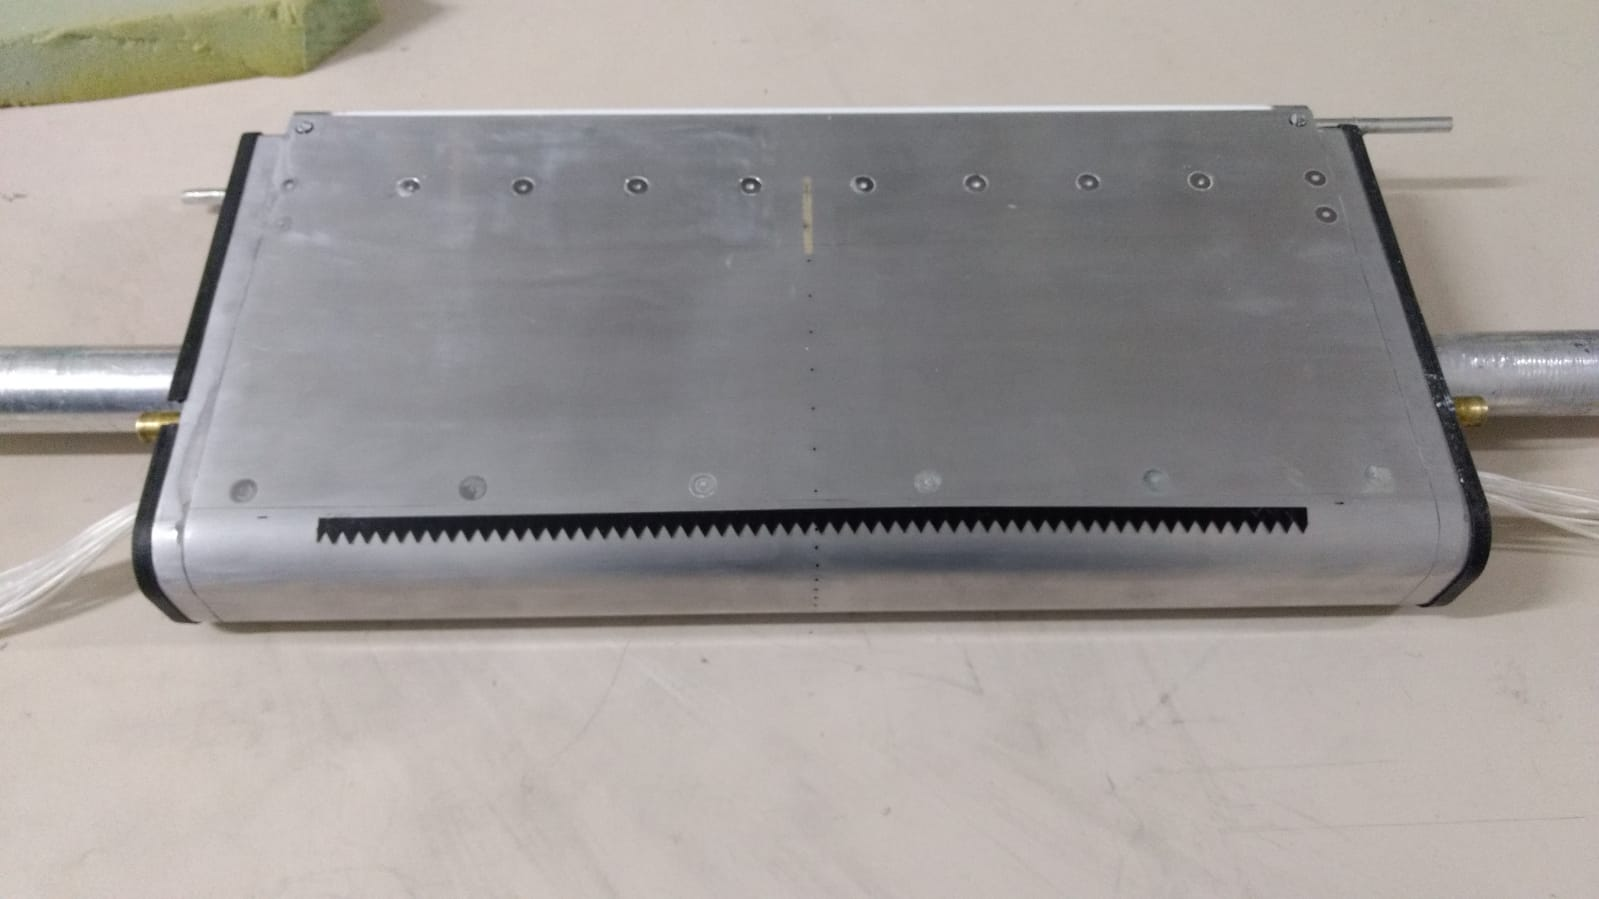
\includegraphics[width=1\textwidth]{DModell1.jpg}
	\caption{Vorderansicht des Versuchsmodells mit angebrachtem Zackenband an Ober- und Unterseite.}
	\label{fig:DModell1}
\end{figure}

%\begin{figure}[h]
%	\centering
%	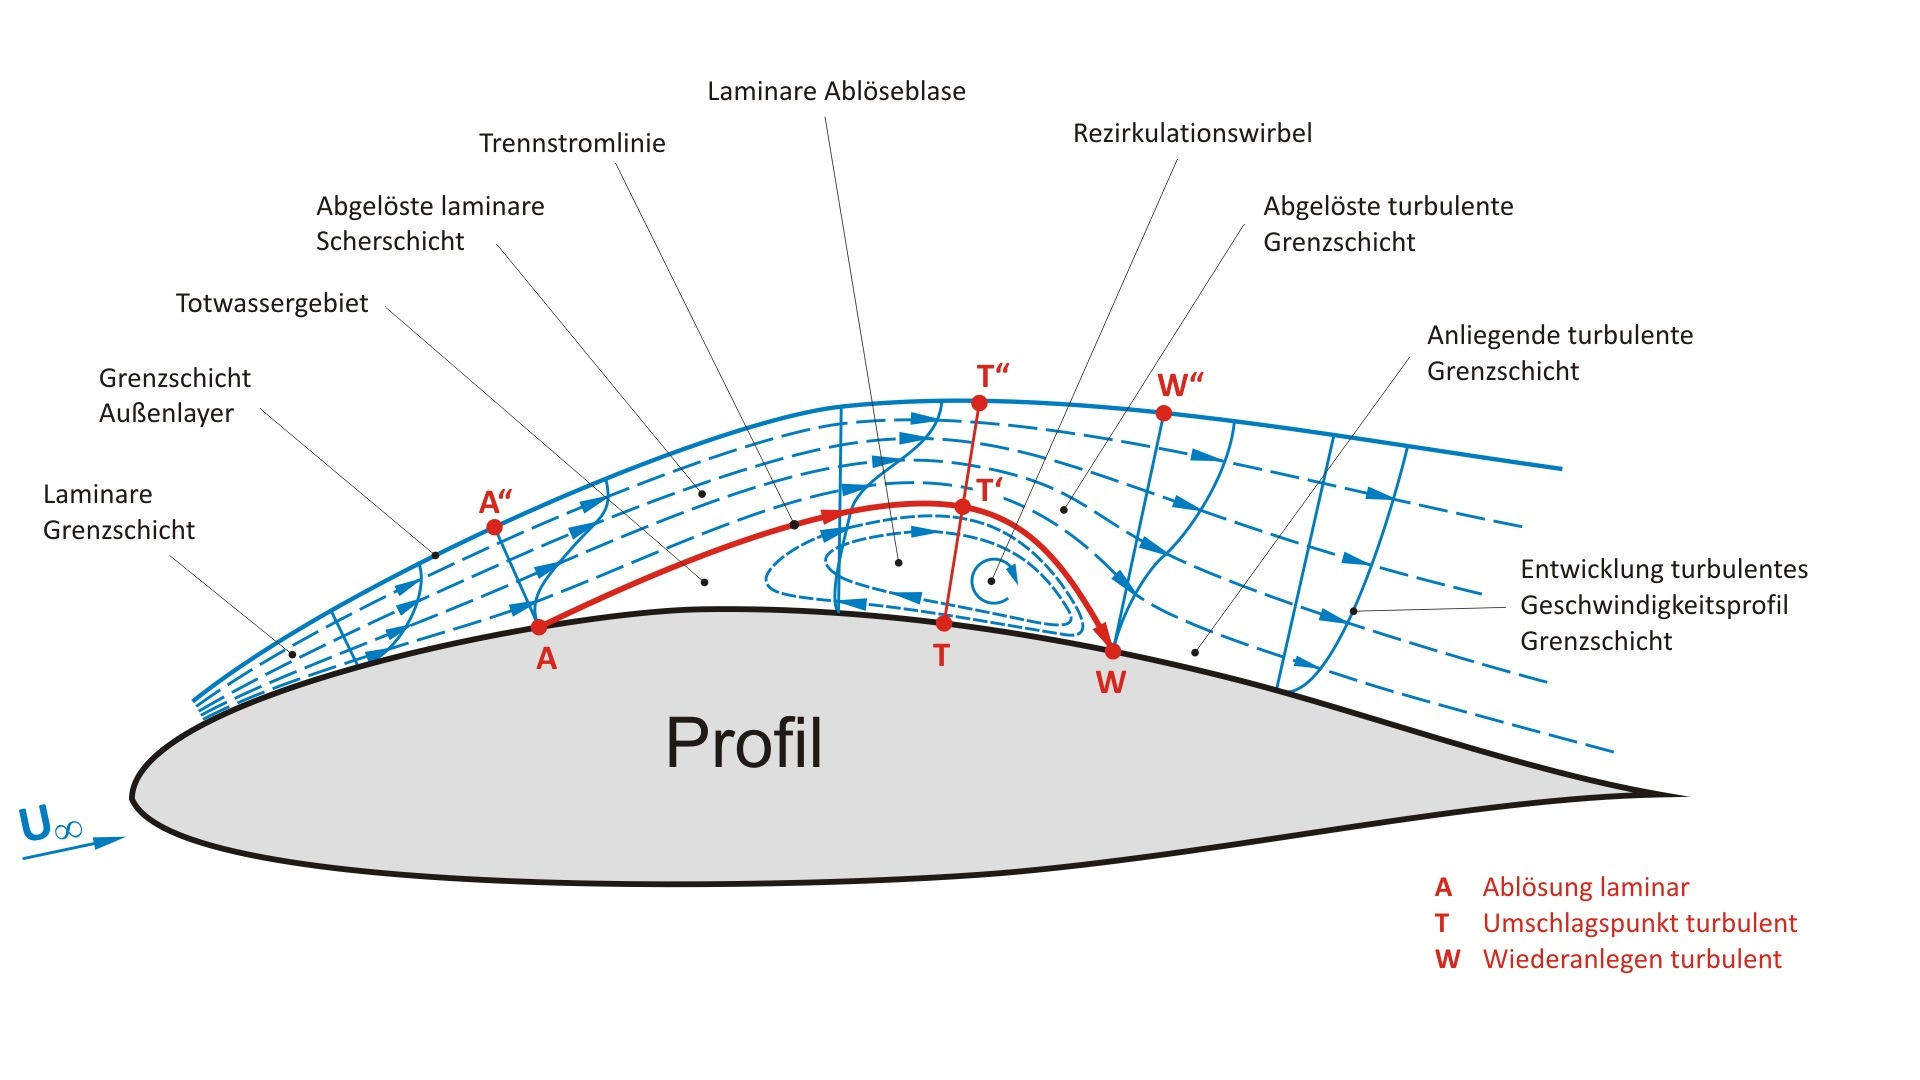
\includegraphics[width=1\textwidth]{LaminareAbloeseblase.jpg}
%	\caption{Schema einer laminaren Abl"oseblase \cite{Mueller.1987}}
%	\label{fig:LamBlase}
%\end{figure}

Wie in \abb{fig:DModell2} ersichtlich ist, sind an der R"uckseite des Stumpfk"orpers an Ober- und Unterseite des Modells jeweils 10 Schrauben montiert. Diese dienen der Einstellung des Ausblasespaltes. Das genaue Verfahren zur Einstellung des Spaltes wird in Abschnitt \ref{sec:Versuchsvorbereitung} erl"autert.


\begin{figure}[h]
	\centering
	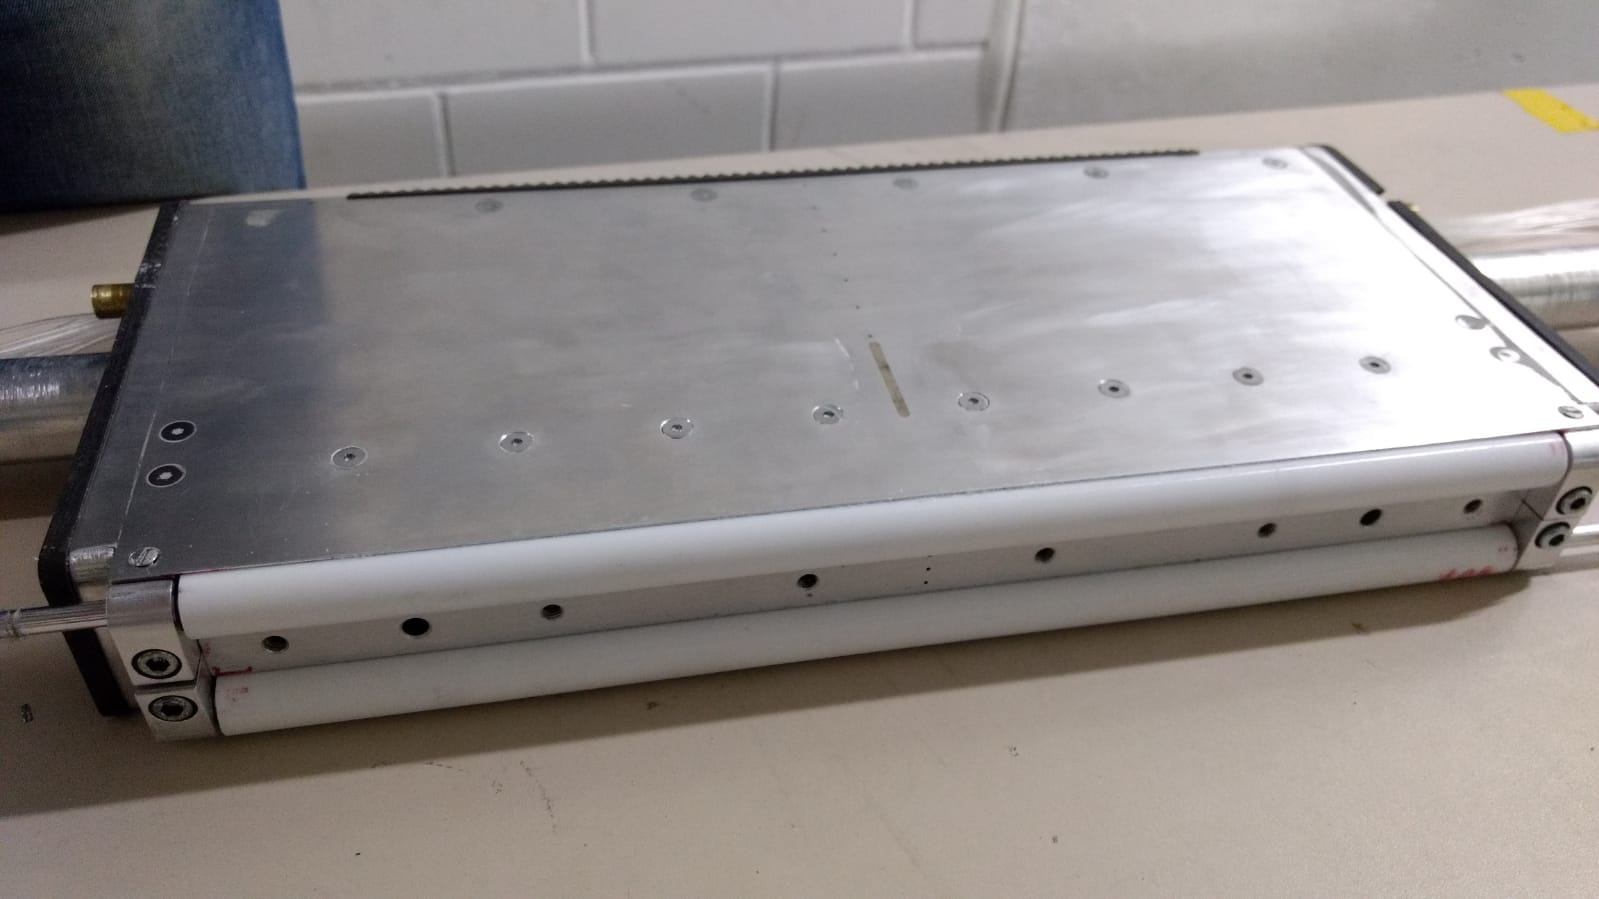
\includegraphics[width=1\textwidth]{DModell2.jpg}
	\caption{R"uckansicht des Versuchsmodells mit eingebauten Tefolnwalzen.}
	\label{fig:DModell2}
\end{figure}

Die Wellen werden seitlich aus dem Windkanal herausgef"uhrt und "uber eine Sicherheitskupplung durch jeweils einen Elektromotor angetrieben. Dies ist in \abb{fig:DModell1} ersichtlich.


\begin{figure}[h]
	\centering
	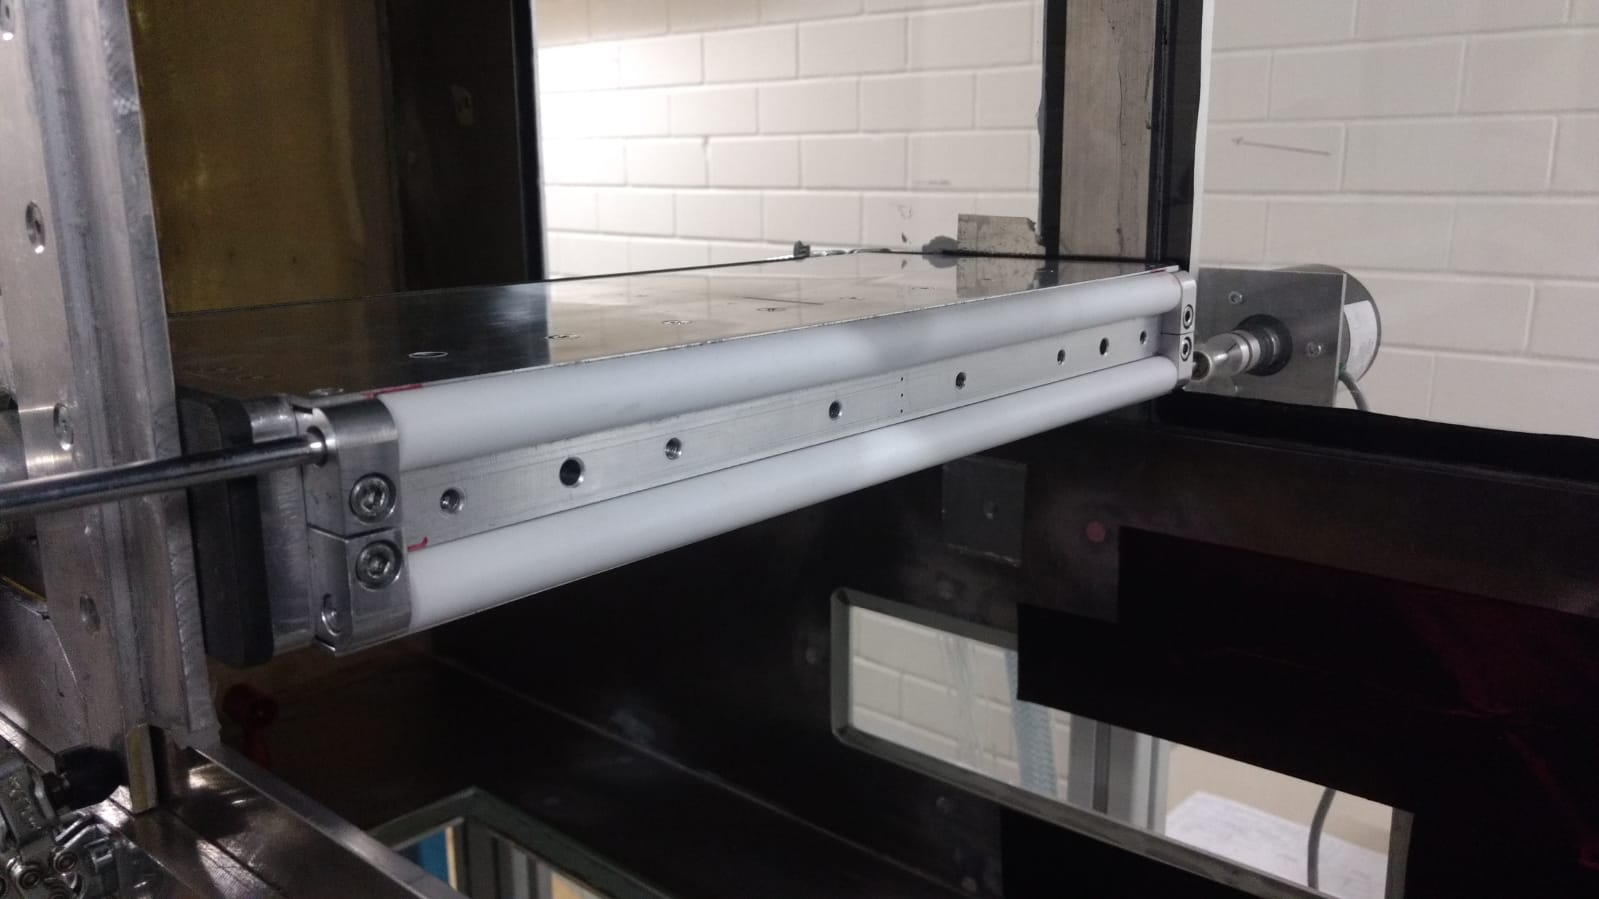
\includegraphics[width=0.8\textwidth]{DModell3.jpg}
	\caption{Versuchsmodell mit eingebauten Teflonwalzen im Windkanal.}
	\label{fig:DModell1}
\end{figure}






\clearpage



%%%%%%%%%%%%%%%%%%%%%%Kebria%%%%%%%%%%%%%%%%%%%%%%%%%%%%%%%%%%%%%

\section{Windkanalbeschreibung (KK)}
F"ur die experimentellen Untersuchungen steht der LNB (Leiser Niedergeschwindigkeitskanal Braunschweig) vom Institut f"ur Str"omungsmechanik der technischen  Universit"at Braunschweig zur Verf"ugung.\\
Dieser ist an beiden Enden offen und wird durch die Umgebungsluft im Raum versorgt, was als Eiffel-Bauart bezeichnet wird. (\abb{fig:windkanal}).
Durch eine besondere Art der Polsterung bzw. Schalld"ampfer und einen
ger"auscharmen Elektroantrieb, ist dieser Windkanal so f"ur einen m"oglichst leisen Betrieb konstruiert worden.
\begin{figure}[h]
	\centering
	\begin{subfigure}[c]{0.5\textwidth}		
		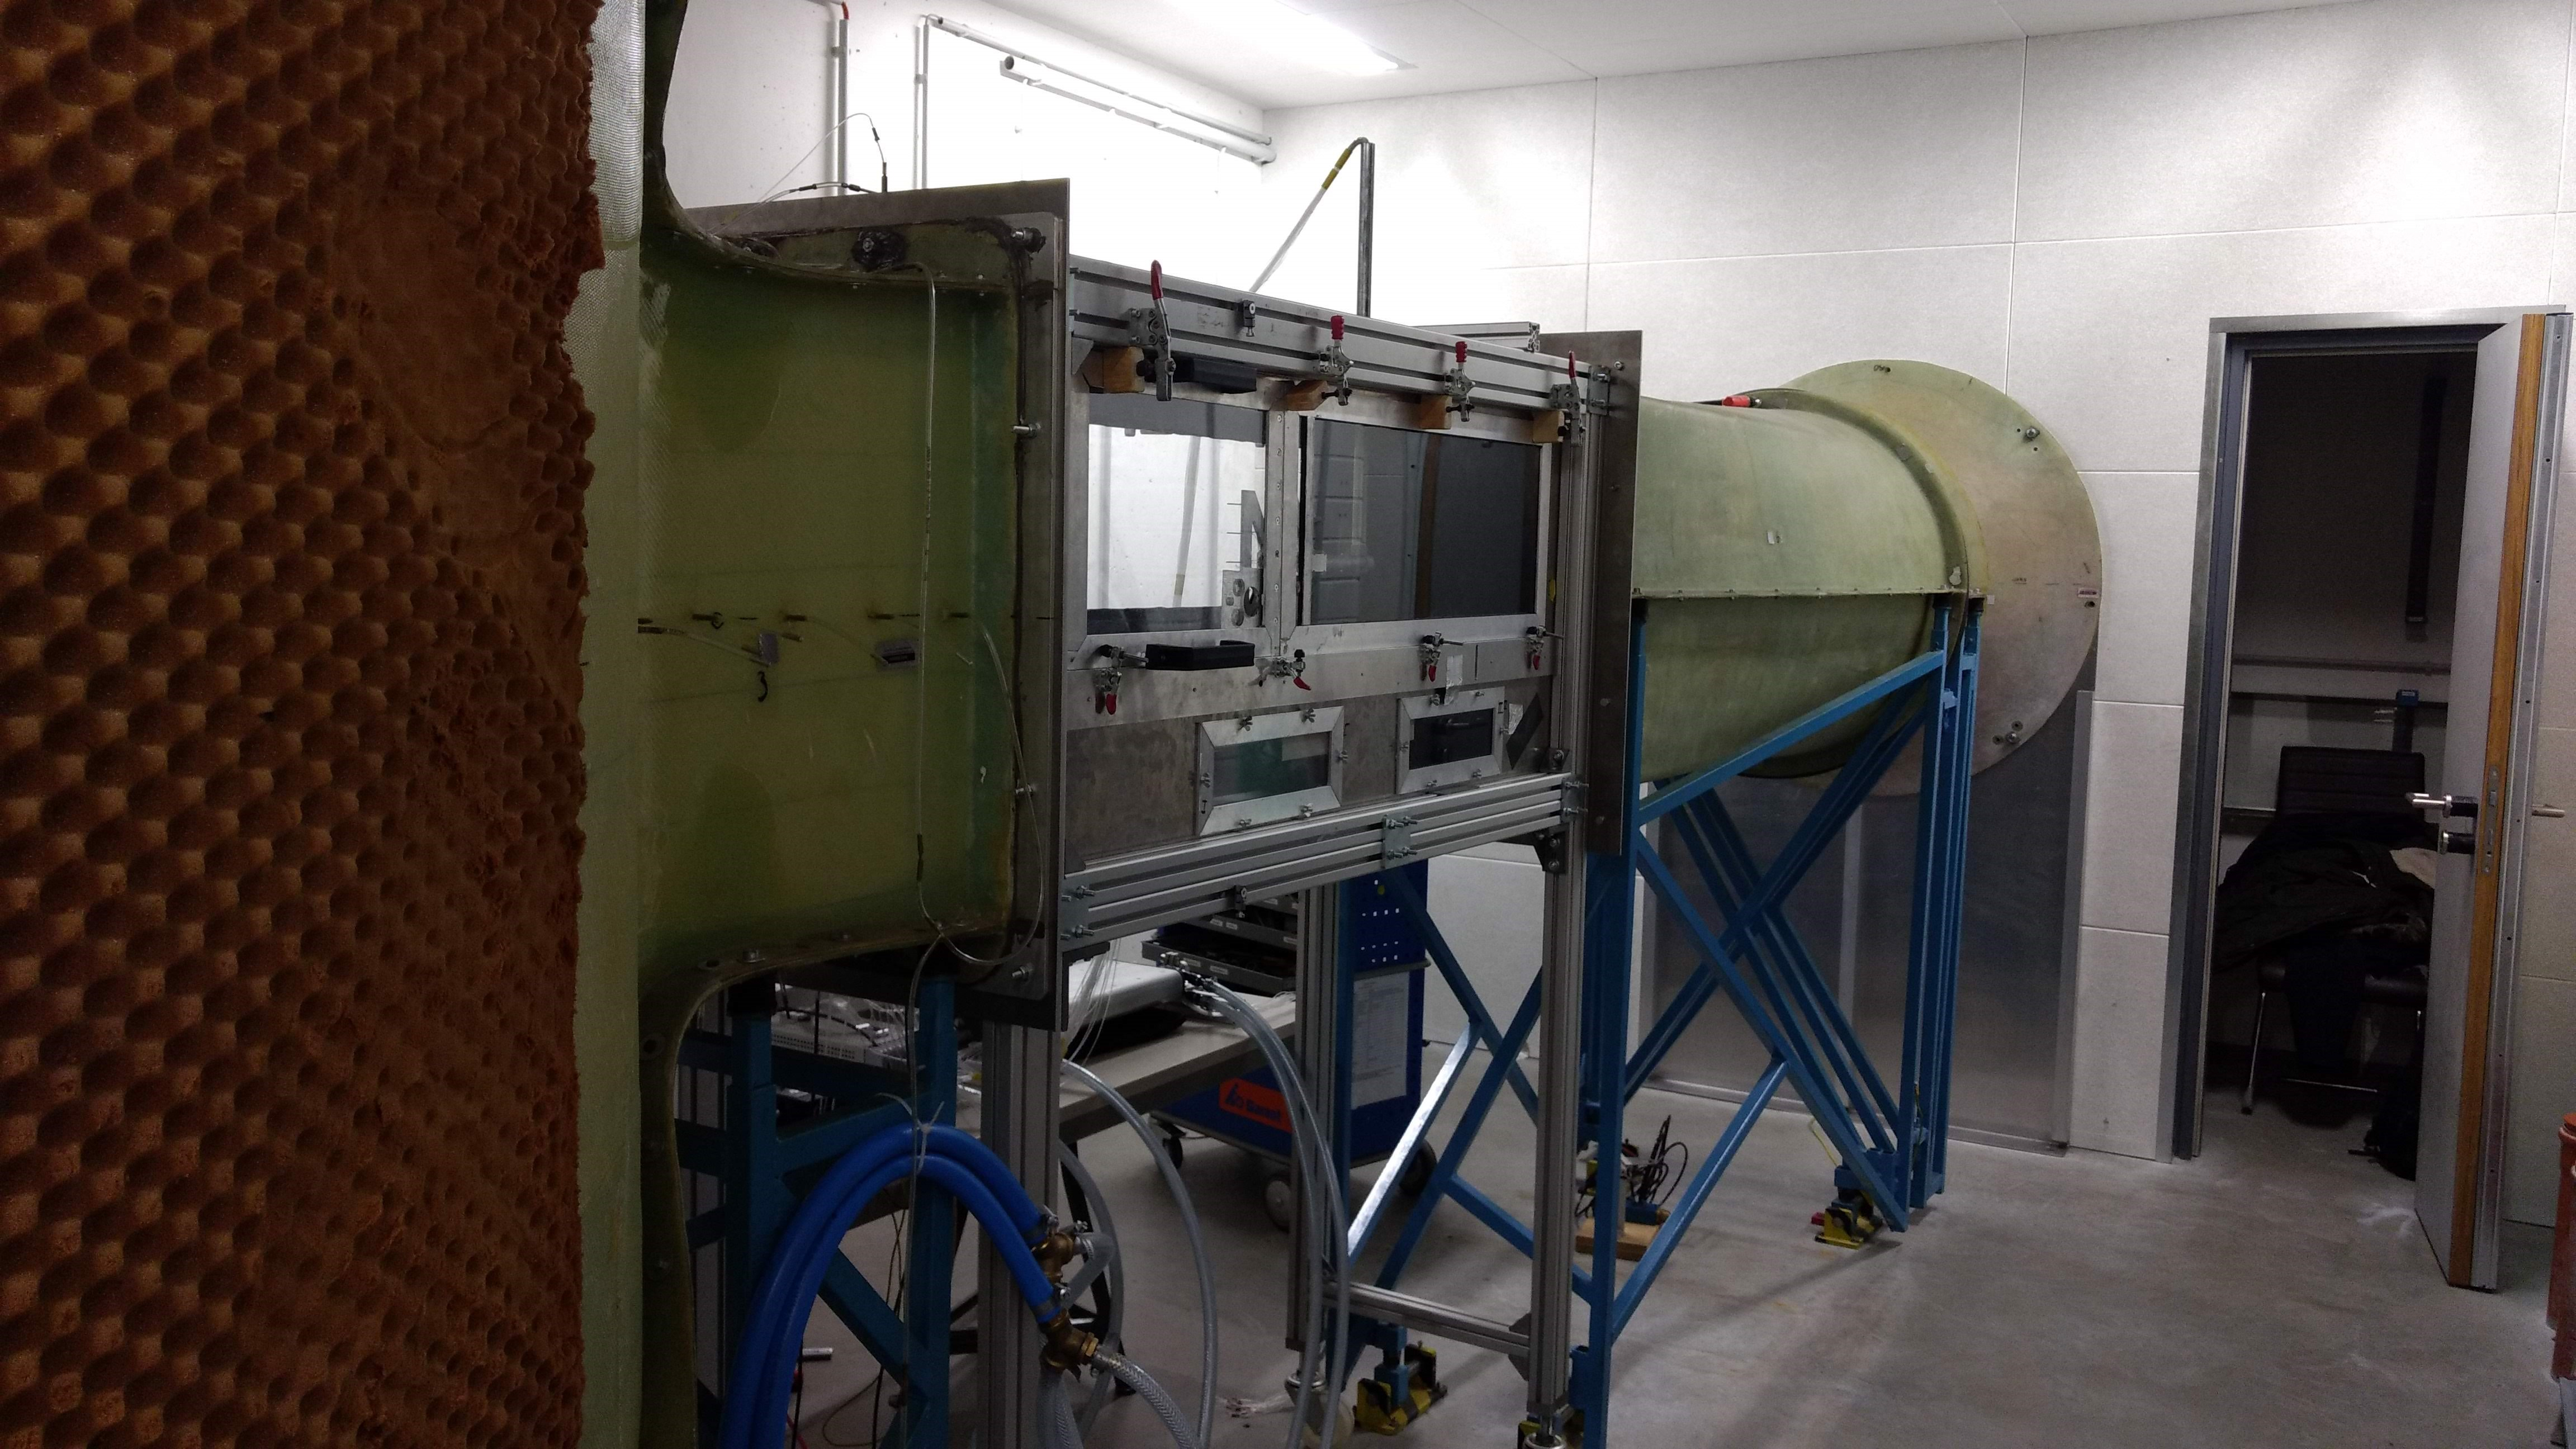
\includegraphics[width=1\textwidth]{windkanal1.jpg}
	\end{subfigure}
	\begin{subfigure}[c]{0.5\textwidth}
		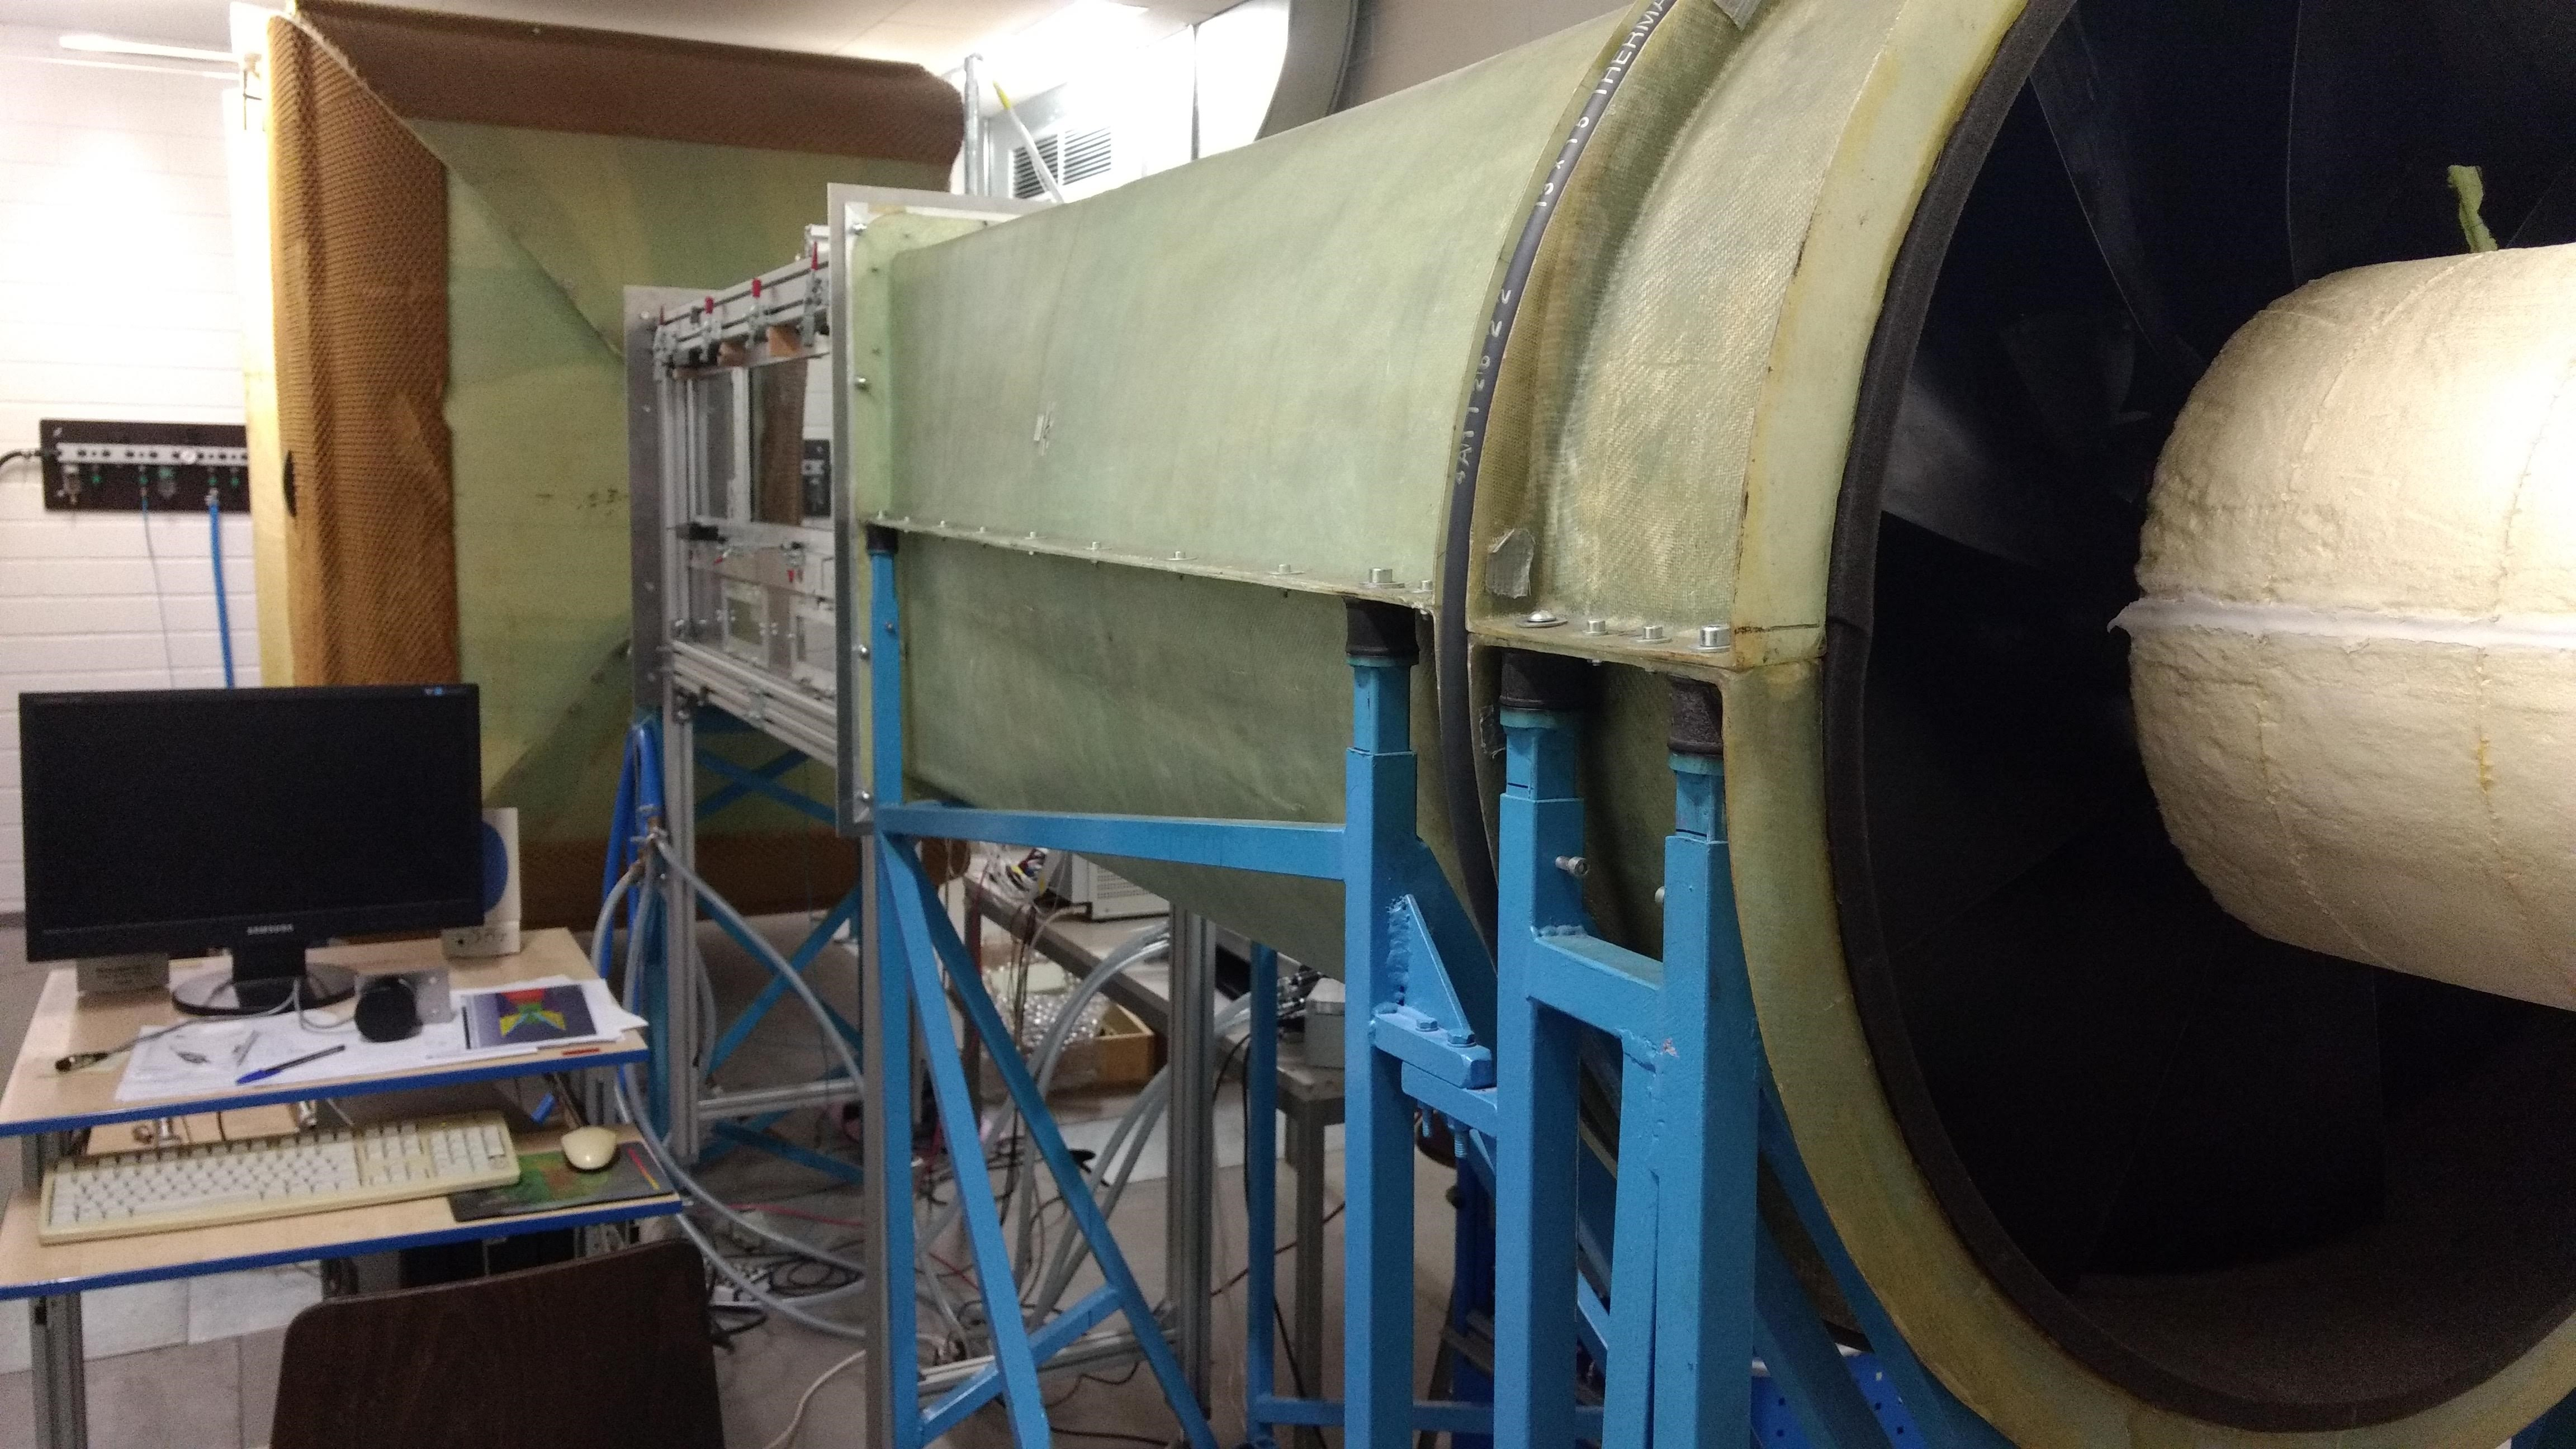
\includegraphics[width=1\textwidth]{windkanal2.jpg}
	\end{subfigure}
	\caption{LNB-ISM TU Braunschweig}
	\label{fig:windkanal}
\end{figure}\\
Testk"orper, die f"ur die Untersuchung eine maximale Anstr"omgeschwindigkeit von \SI{20}{\meter/\second} ben"otigen und die passende Gr"o\ss{}e haben, sind f"ur Versuche in diesem Windkanal geeignet.

\section{Messtechnik (KK)}
Nicht nur bei der Versuchsvorbereitung, sondern auch w"ahrend des Versuchs werden Messger"ate und Einrichtungen ben"otigt, ohne die eine sinnvolle Untersuchung und rechnerische Ermittlungen der Versuchsparameter nicht m"oglich ist.

Hier wird auf die f"ur den Versuch eingesetzten Messmittel und deren Funktionsweisen eingegangen.

\subsection{Messuhr}
Die Messuhr wird f"ur die Messung der L"angendifferenzen oder auch L"angen eingesetzt. Mit einer "ublichen Genauigkeit von \SI{10}{\micro\meter} und einem Messbereich von 5 bis \SI{60}{\milli\meter} eignen sich die Messuhren f"ur Parallelit"ats- und Ebenheitsmessungen.

\subsection{Fischmaul-Sonde}
Die Fischmaul-Sonde ist im Prinzip ein an der Spitze plattgedr"ucktes Pitot-Rohr. Sie eignet sich am besten f"ur Staudruckmessungen an bzw. in angestr"omten Spalten.

\subsection{Statische Sonde}
Die statische Sonde besitzt nur Bohrungen, die tangential zur Str"omung sind und deshalb nur für die Messung des statischen Drucks geeignet sind.
Damit die Bohrungen m"oglichst keinen dynamischen Anteil messen, m"ussen sie sich weit genug entfernt von der Sondenspitze befinden, da in und nach diesem Bereich, die Str"omung umgelenkt wird und lokal nicht mehr tangential zu den Bohrungseintrittsfl"achen steht.

\subsection{Prandtl-Sonde}
Diese Sonde kombiniert die statische Sonde und das Pitot-Rohr.
Die von der seitlichen Bohrungen gemessenen Dr"ucke laufen im inneren System gegen den an der Spitze gemessenen Staudruck.
Somit wird der statische Druck vom Gesamtdruck abgezogen und der dynamische Druck erhalten. Durch weitere Rechnungen ist es m"oglich, mittels dynamischen Drucks die Anstr"omgeschwindigkeiten zu berechnen.

\subsection{Drehzahlmesser}

\subsection{PSI-Anlage}

\section{Versuchsvorbereitung (KK)}
\label{sec:Versuchsvorbereitung}


\chapter{Versuchsauswertung}
\label{s:auswertung}
\section{Einleitung (KK)}
\label{s:einleitungAusw}
Um den Einfluss der widerstandsreduzierenden Effekte bestimmen zu k"onnen, werden beide Wellenpaare bei 3  verschiedenen Konstellationen getestet. So kann die Effektivit"at von der Ausblasung und der Rotation erst separat und dann in Kombination untersucht werden.
Alle Messungen werden bei einer vorbestimmten Reylondszahl von 50000 durchgef"uhrt.
Im folgenden Diagramm ist die Nachlaufdelle bei dem D-f"ormigen Stumpfk"orper ohne jegliche widerstandsreduzierenden Ma\ss{}nahmen zu sehen. 
Es wird erwartet, dass die Nachlaufdelle durch die zu untersuchenden Effekte kleiner wird.
\begin{figure}[h]
	\centering
	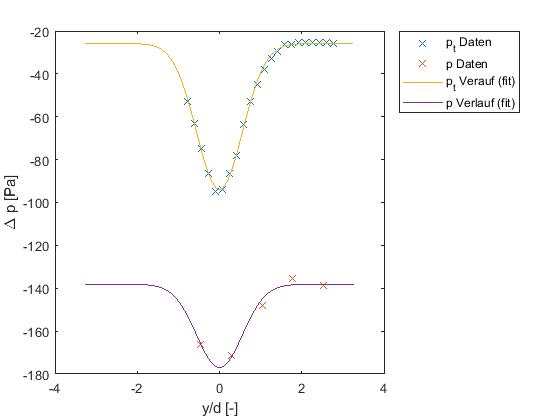
\includegraphics[width=0.75\textwidth]{Druckverlaeufe_Nachlauf_ohneAkt.jpg}
	\caption{ $\Delta P$ "uber y/d ohne Aktuierung }
	\label{fig:Deltap-y/d_ohne_Aktuation}
\end{figure}
\\
Bei den Versuchsreihen mit den ovalen Wellen muss darauf geachtet werden, dass untere und obere Welle das Signal phasengleich generieren. Allerdings konnte diese Phasengleichheit wegen der limitierten Zeit dieser Arbeit nur durch mehrere Messungen f"ur jede Parameterkombination angen"ahert werden.
F"ur genauere Ergebnisse, die besser reproduziert werden k"onnen, w"aren verschiedene "Anderungen am Versuchsaufbau denkbar beispielsweise k"onnten die beiden Wellen mechanisch "uber Zahnriemen oder "ahnliche Konstruktionen  miteinander verbunden werden. Eine andere Variante w"urde neben der Drehzahl der Motoren auch die Auslesung von Signalen "uber die Phasen  vorsehen, wodurch eine Synchronisation vereinfacht werden kann.
Au\ss{}erdem ist es erw"ahnenswert, dass die Ergebnisse von dem Versuch mit der Konfiguration 50, von der Realit"at bzw. der Annahme abweichen, da die Teflonschicht aufgrund
gro\ss{}er Reibungskr"afte "uberbelastet wurde, und sich teilweise abgespant hat (Siehe Abbildung).
Dies f"uhrt dazu, dass der Ausblasespalt nicht vollst"andig geschlossen wird und der vorbestimmte Signalverlauf nicht erreicht wird.
Um dies zu vermeiden, k"onnen die Wellen aus anderen h"arteren und/oder reibungs"armeren Materialien gebaut werden, oder das Material der Ausblaselippe mit dem der Wellen vertauscht werden. Au\ss{}erdem k"onnen Alternativen f"ur die Schlie\ss{}ung des Ausblasespaltes gefunden werden. Eine M"oglichkeit w"are, den Spalt kontaktlos durch das Ph"anomen "Verstopfung" zu schlie\ss{}en.
\begin{figure}[h]
	\centering
	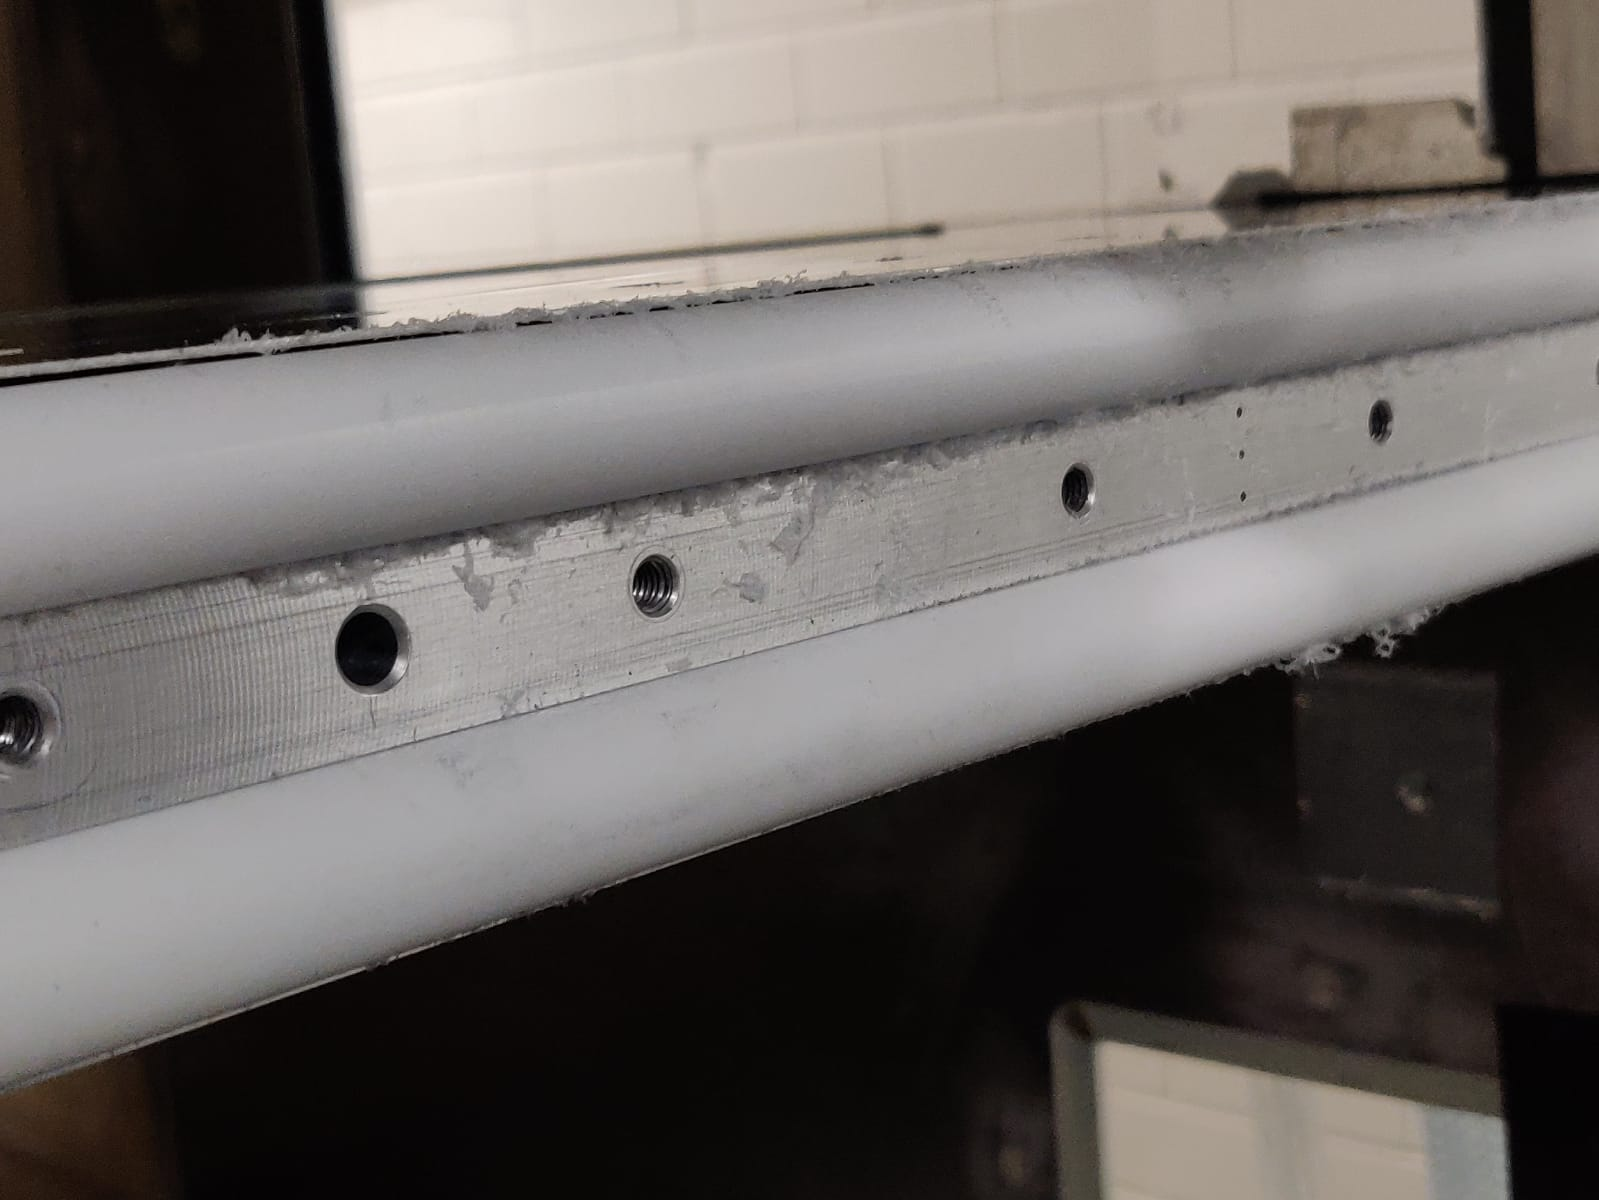
\includegraphics[width=0.75\textwidth]{Materialabrieb.jpeg}
	\caption{ Materialabrieb an der Teflonschicht }
	\label{fig:Materialabrieb}
\end{figure}



\section{Konstellation 1: Reine Rotation (KK)}
\label{s:ReineRotation}

In  \abb{fig:Cw-n_Rein_Konf+2} sind die Widerstandsbeiwerte von beiden Wellenpaaren bei verschiedenen Wellendrehzahlen zu sehen.
Die nat\"urliche Abl\"osefrequenz wird bei einer Drehzahl von 1938 1/min  erreicht. F\"ur eine gute Vergleichbarkeit wird der Bereich vor und insbesondere nach dieser Drehzahl, sowohl bei den glatten als auch bei den gezahnten Wellen genauer und hochaufl\"osender untersucht.
Abgesehen davon, dass die Konfiguration mit den ovalen bzw. gezahnten Wellen, in allen Drehzahlbereichen einen geringeren $C_{w}$-Wert im Vergleich zur Basiskonfiguration aufweisen, ist das Verhalten der beiden Kurven jedoch unterschiedlich.
\begin{figure}[h]
	\centering
	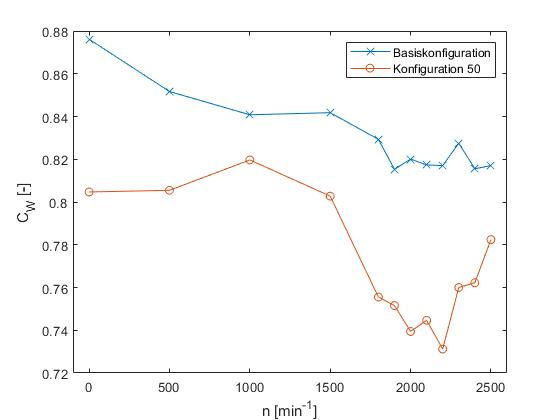
\includegraphics[width=0.5\textwidth]{Cw_ueber_n_ohneAB_beideKonf.jpg}
	\caption{ $C_{w}$-n reine Rotation beide Wellenpaare }
	\label{fig:Cw-n_Rein_Konf+2}
\end{figure}

W\"ahrend der $C_{w}$-Wert bei der Basiskonfiguration direkt nach der Impulsbeaufschlagung der Grenzschicht durch Rotation der Wellen zu sinken anf\"angt, steigt der $C_{w}$-Wert der Konfiguration mit gezahnten Wellen bis zu einer Drehzahl von 1000 1/min. Erst ab einer Drehzahl von 1500 1/min, ist eine deutliche Widerstandsreduzierung zu erkennen. 
Anders als die Basiskonfiguration, bei der der minimale $C_{w}$-Wert im Bereich der erwarteten Abl\"osefrequenz erreicht wird, geschieht dies bei der Konfiguration 50 nach der Abl\"osefrequenz und zwar bei ca. n= 2200. 
Beide Verl\"aufe steigen wieder, nachdem der niedrigste $C_{w}$-Wert erreicht wurde. Dennoch ist diese
Steigung mit den ovalen Wellen deutlich gr\"o\ss{}er und drehzahlsensibler.
Um von der Widerstandsreduzierung profitieren zu k\"onnen, muss noch genau verglichen werden, wie viel Leistung die jeweilige Konfiguration in Anspruch nimmt. Diese wird mit der kinetischen Leistung der Hauptstr\"omung genormt und als Leistungskoeffizient bezeichnet.

In \abb{fig:Cw-Cw0-CpowerM_reine} ist das $C_{w}$/$C_{w0}$-$C_{Power}$-Diagramm zu sehen. Es ist deutlich erkennbar, dass die ovalen Wellen, wesentlich mehr Energie ben\"otigen, um die Reibung zwischen der Teflonoberfl\"ache und dem Ausblaseschlitz zu \"uberwinden. Dazu kommt, dass die ovalen Wellen bei niedrigen Drehzahlen erst eine Widerstandssteigerung verursachen. 

Bei der Basiskonfiguration sinkt der $C_{w}$/$C_{w0}$-Wert, bereits bei geringer Energiezufuhr.  Nachdem der niedrigste Widerstandsbeiwert bei einer $C_{Power}$= 0,2 erreicht wurde, f\"angt die Kurve an, lokal zu schwanken. Dies kommt durch die hohe lokale Drehzahlaufl\"osung im Bereich der Abl\"osefrequenz zustande. Laut Diagramm w\"urde es sich nicht lohnen, die glatten Wellen mit einer h\"oheren Drehzahl als 1900  1/min zu drehen, da bei weiterer Energiezufuhr, keine Widerstandsreduzierung zu erkennen ist.
\begin{figure}[h]
	\centering
	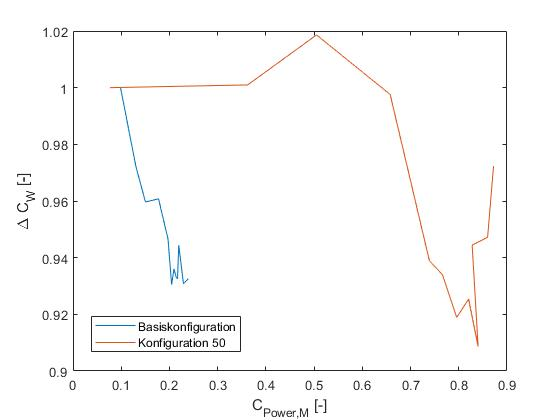
\includegraphics[width=0.5\textwidth]{DeltaCw_ueberC_PowerM_ohne_AB_beideKonf.jpg}
	\caption{ $C_{w}$/$C_{w0}$ \"uber $C_{Power,M}$ f\"ur reine Rotation  }
	\label{fig:Cw-Cw0-CpowerM_reine}
\end{figure}
Bei der Konfiguration mit den ovalen Wellen muss deutlich mehr Leistung aufgebracht werden, um eine Widerstandsreduzierung im Vergleich zu der Konfiguration ohne Aktuieren zu erhalten.  Erst ab einem $C_{Power}$ von ca. 0,65 wird ein $C_{w}$/$C_{w0}$ erreicht, der kleiner als 1 ist. 
Danach sinkt der $C_{w}$-Wert stark und erreicht den kleinsten $C_{w}$-Wert bei einem $C_{Power}$= 0,84. 
Der minimale $C_{w}$/$C_{w0}$ ist zwar kleiner als bei der Basiskonfiguration und somit die Widerstandsreduzierung gr\"o\ss{}er, jedoch muss deutlich mehr Leistung aufgebracht werden.
\begin{table}[h]
	\centering
	\begin{tabular}{lrr}
		\toprule
		 & kleinster  $C_{w}$/$C_{w0}$ & $C_{Power}$ beim kleinsten $C_{w}$/$C_{w0}$ \\
		\midrule
		Basiskonfiguration & 0.93 & 0.2\\
		Konfiguration 50 & 0.91 & 0.84\\
		\bottomrule
	\end{tabular}\\
	\caption{ minimale  $C_{w}$-Werte und die entsprechenden $C_{Power}$ }
	\label{tab:minimalCw-Cpower}
\end{table}
Der Tabelle 6.5 zu entnehmen, muss man die Leistung um 420\% steigern, um mit den ovalen Wellen einen um ca. 2\% geringeren $C_{w}$/$C_{w0}$ als die Basiskonfiguration zu bekommen.

%%%%%%%%%%%%%%%%%%%%%%%%%%%%%%%%%%%%%%%%%%%%%%%%%%%%%%%%%%%%%%%%%%%%%%%%%%%%%%%%%%%%%%%%%%%%%%%%%%%%%%%%%%%

\section{Konstellation 2: Reine Ausblasung (AK)}
\label{s:reineAusblasung}
In diesem Abschnitt wird das Profilmodell mit den glatten Welle und die Konfiguration 50 bei reiner Ausblasung betrachtet. Die Rotation bei den Wellen spielt hier somit keine Rolle. 

Der Volumenstrom wurde bei den glatten Wellen so eingestellt, dass
die folgenden $C_{\mu}$  Werte erreicht werden. Es wurde $C_{w}$ mit diesen vier verschiedenen $C_{\mu}$ Werte gemessen.Die Ergbnisse sind wie folgt:
\begin{table}[H]
	\centering
	\begin{tabular}{lr}
		\toprule
		$C_{\mu}$ & $C_{w}$ \\
		\midrule
		0.00 & 0.876\\
		0.16 & 0.606\\
		0.32 & 0.477\\
		0.48 & 0.399\\
		0.69 & 0.331\\
		\bottomrule
	\end{tabular}
	\caption{$C_{w}$ und $C_{\mu}$ mit der glatten Welle ohne Aktuation }
	\label{tab:Cw-Cmu_Kon1}
\end{table}
Diese Impulskoeffizienten sind so gew"ahlt, dass man die Ergebnisse mit der Arbeit von \textit{Bilges} vergleichen kann.

Die \abb{fig:Cw-Cmu_Konf1} zeigt die Funktion von Widerstandsbeiwert \"uber Impulsbeiwert f\"ur die glatten Wellen ohne Rotation:
\begin{figure}[h]
	\centering
	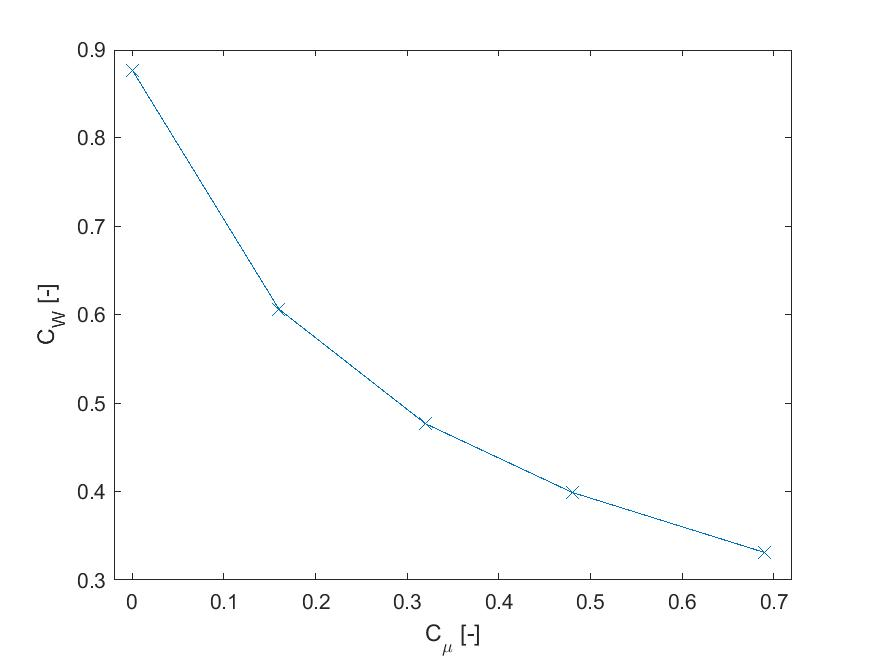
\includegraphics[width=0.5\textwidth]{Cw_ueber_Cmu_ohne_n.jpg}
	\caption{$C_{w}$  \"uber $C_{\mu}$ mit den glatten Wellen ohne Rotation }
	\label{fig:Cw-Cmu_Konf1}
\end{figure}

Aus der \abb{fig:Cw-Cmu_Konf1} ist ein deutlicher Abfall von $C_{w}$ mit steigendem $C_{\mu}$ ersichtlich.

F\"ur den Versuch mit den ovalen Wellen werden  $C_{\mu}$ Werte f\"ur die Verschiedenen Luftdr\"ucke berechnet, die eingestellt worden sind. In \tab{tab:Cw-Cmu_Konf1+2} sind die Auswertungen f\"ur $C_{w}$ zu sehen. 
\begin{table}[h]
	\centering
	\begin{tabular}{lrr}
		\toprule
		Luftdruck [kPa] & $C_{\mu}$ & $C_{w}$ \\
		\midrule
		0 & 0.00 & 0.805\\
		1 & 0.06 & 0.610\\
		2 & 0.27 & 0.594\\
		3 & 0.42 & 0.577\\
		4 & 0.58 & 0.455\\
		\bottomrule
	\end{tabular}\\
	\caption{Luftdruck, $C_{w}$  und $C_{\mu}$ f\"ur die glatten und ovalen Wellen ohne Rotation}
	\label{tab:Cw-Cmu_Konf1+2}
\end{table}

Die \abb{fig:Cw-Cmu_Konf1+2} zeigt den Verlauf $C_{w}$ \"uber $C_{\mu}$ f\"ur die beiden Konfigurationen.
\begin{figure}[h]
	\centering
	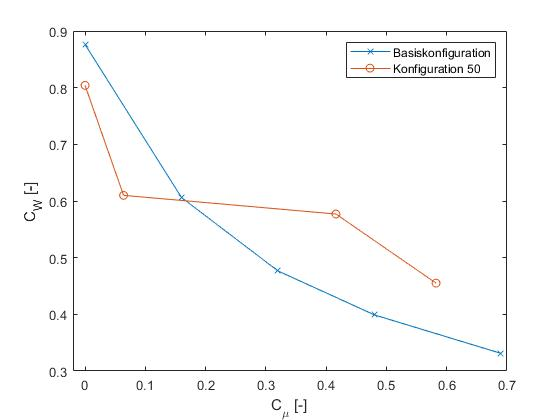
\includegraphics[width=0.5\textwidth]{Cw_ueber_Cmu_ohne_n_beideKonf.jpg}
	\caption{$C_{w}$  \"uber $C_{\mu}$ mit den glatten Wellen ohne Aktuation }
	\label{fig:Cw-Cmu_Konf1+2}
\end{figure}

Wie man im Diagramm sieht, f\"allt auch bei der Konfiguration mit ovalen Wellen  $C_{w}$  mit steigendem $C_{\mu}$.\\
Im Vergleich mit den glatten Wellen sind die Widerstandsbeiwerte bei Impulskoeffizienten im Bereich von 0 bis 0.16  bei den ovalen Wellen niedriger. Aber ab dem Punkt $C_{\mu}$= 0.16 sinkt der Widerstandsbeiwert der glatten Wellen st\"arker ab. Aus diesem Grund sind die glatten Wellen ohne Rotation bei den gr\"o\ss{}eren Impulskoeffizienten der Konfiguration 50 vorzuzi.

Die \tab{tab:Cw/Cw0-CpJet_Kon1} zeigt den Leistungskoeffizienten der Ausblasung in Abh"angigkeit der genormten $C_W$-Werte der Basiskonfiguration. Die Normierung erfolgt hierbei durch den Widerstandsbeiwert von der jeweiligen Konfiguration komplett ohne Aktuation.
\begin{table}[h]
	\centering
	\begin{tabular}{lr}
		\toprule
		$C_{w}$/$C_{w0}$ & $C_{Power,Jet}$ \\
		\midrule
		1 & 0\\
		0.691 & 0.010\\
		0.544 & 0.283\\
		0.455 & 0.520\\
		0.378 & 0.896\\
		\bottomrule
	\end{tabular}
	\caption{$C_{w}$/$C_{w0}$ \"uber $C_{Power,Jet}$ f\"ur Basiskonfiguration }
	\label{tab:Cw/Cw0-CpJet_Kon1}
\end{table}

Und die Auswertungen f\"ur die Konfiguration mit den ovalen Wellen sind in der Tabelle 6.4:

\begin{table}[h]
	\centering
	\begin{tabular}{lr}
		\toprule
		$C_{w}$/$C_{w0}$ & $C_{Power,Jet}$ \\
		\midrule
		1 & 0\\
		0.748 & 0.149\\
		0.718 & 0.773\\
		0.566 & 1.90\\
		\bottomrule
	\end{tabular}
	\caption{$C_{w}$/$C_{w0}$ \"uber $C_{Power,Jet}$ f\"ur die ovalen Wellen }
	\label{tab:Cw/Cw0-CpJet_Kon2}
\end{table}

Die \abb{fig:Cw/Cw0-CpJet_Konf1+2} zeigt den Verlauf $C_{w}$/$C_{w0}$ \"uber $C_{Power,Jet}$  f\"ur die beiden Konfigurationen:
\begin{figure}[h]
	\centering
	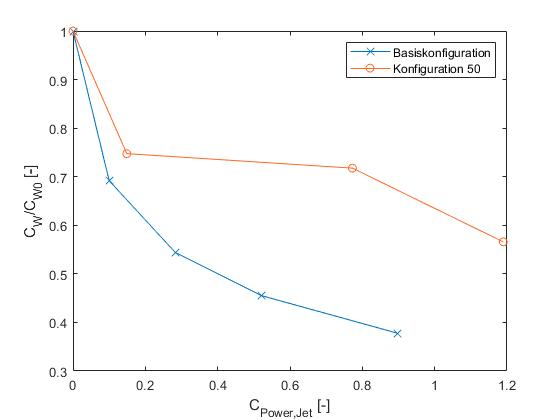
\includegraphics[width=0.5\textwidth]{CwC0_ueber_CPowerJ_ohne_n_beideKonf.jpg}
	\caption{$C_{w}$/$C_{w0}$  \"uber $C_{Power,Jet}$ f\"r die beiden Konfigurationen}
	\label{fig:Cw/Cw0-CpJet_Konf1+2}
\end{figure}

Wie aus dem Diagramm ersichtlich ist, wird mehr Leistung ben\"otigt, um einen niedriegen Wiederstansbeiwert $C_{w}$  zu erreichen. Mit den ovalen Wellen wird mehr Leistung als den glatten Wellen ben\"otigt, um die gleiche Widerstandsreduzierung zu erzielen. Deswegen weist die Konfiguration mit den glatten Wellen in diesem Fall bessere Ergebnisse auf.
\newpage

\section{Konstellation 3: Kombinierte Aktuation (KK)}
\label{s:kombinierteAkt}
Nun wird bei beiden Konfigurationen sowohl durch die Walzen als auch durch die Ausblasung aktuiert.

Die in \kap{s:reineAusblasung} verwendeten $C_{\mu}$-Werte f"ur die Konfiguration mit ovalen Wellen beziehen sich auf eine Wellenstellung, bei der der Spalt maximal ge"offnet ist, die Spalth"ohe also ca. 0,3\,mm betr"agt. Diese Position kann als einzige ge"offnete Wellenposition definiert eingestellt werden und dient der besseren Vergleichbarkeit mit der Basiskonfiguration. Wenn die Rotation hinzugenommen wird, "andert sich das $C_{\mu}$ allerdings und muss nach \glg{eq:momentum-coeff-oscill-final} berechnet werden. Die mit dem urspr"unglichen Impulskoeffizienten korrespondierenden neuen $C_{\mu}$-Werte sind in \tab{tab:Cmu Korrektur} festgehalten.

\begin{table}[H]
	\centering
	\begin{tabular}{lr}
		\toprule
		$C_{\mu}$ (reine Ausblasung) & $C_{\mu}$ (kombinierte Aktuation)\\
		\midrule
		0 & 0\\
		0,064 & 0,097\\
		0,27 & 0,231\\
		0,416 & 0,29\\
		0,582 & 0,327\\
		\bottomrule
	\end{tabular}
	\caption{Korrespondierende $C_{\mu}$-Werte f"ur reine Ausblasung und kombinierte Aktuation bei Konfiguration 50}
	\label{tab:Cmu Korrektur}
\end{table}


F"ur die Betrachtungen und Abbildungen wird aus "Ubersichtlichkeitsgr"unden das urspr"ungliche $C_{\mu}$ verwendet. Dieser Zusammenhang erschwert die Interpretation allerdings und muss stets ber"ucksichtigt werden.

Die Vergleichbarkeit mit der Basiskonfiguration ist hier zus"atzlich dadurch eingeschr"ankt, dass nur bis zum mittleren Plenumsdr"ucken von 4\,kPa gemessen wurde und die Impulskoeffizienten f"ur diese Konfiguration nicht die der Basiskonfiguration erreichen.\\
H"ohere Dr"ucke k"onnen gleichwohl nicht mitbetrachtet werden, da bei einem d"unnen verbleibenden Spalt die Dr"ucke deutlich "uber 9\,kPa liegt, was wiederum in Jetgeschwindigkeiten oberhalb $Ma =$ $\frac{1}{3}$ m"undet. Die Annahme der inkompressiblen Jetstr"omung kann dann nicht mehr getroffen werden.

In \abb{fig:Cw/n bei Cmu RK} ist $C_{W}$ "uber n bei verschiedenen $C_{\mu}$ f"ur die Basiskonfiguration dargestellt.

\begin{figure}[h]
	\centering
	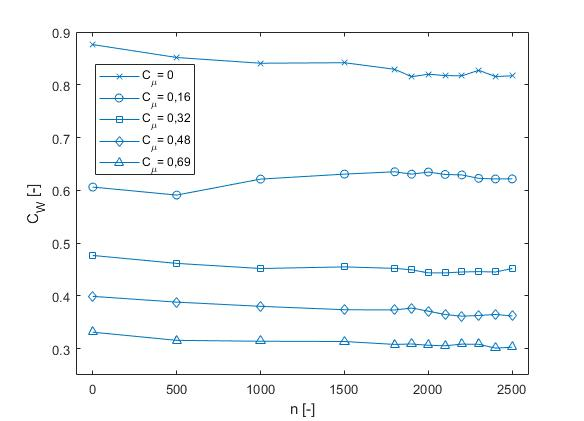
\includegraphics[width=0.5\textwidth]{Cw_ueber_n_fuer_verschiedeneCmu_RK.jpg}
	\caption{$C_{w}$ "uber $n$ bei verschiedenen $C_{\mu}$ f"ur die Basiskonfiguration}
	\label{fig:Cw/n bei Cmu RK}
\end{figure}

Au\ss{}er bei $C_{\mu}= 0,16$ sind alle anderen Verl"aufe in Abh"angigkeit von der Drehzahl "ahnlich.
Sie sinken mit einer "ahnlichen Rate bis zum Bereich der nat"urlichen Abl"osefrequenz und schwanken leicht wachsend danach.\\Mit einem $C_{\mu}= 0,16$ wird der $C_{W}$-Verlauf bis auf $n= 500$, wo der Widerstand minimal reduziert wird, immer oberhalb des $C_{W}$ der reinen Ausblasung gehalten. In diesem Fall bedeutet eine zus"atzliche Rotation mehr Energie und Aufwand, und steigert den Widerstandsbeiwert.

Bei der Betrachtung der $C_{W}-n$-Verl"aufe in Abh"angigkeit von den Impulskoeffizienten ist ersichtlich, dass diese mit steigendem $C_{\mu}$ degressiv sinken und eine Ausblasung unabh"angig von der Drehzahl einen gro\ss{}en Anteil an der Widerstandsreduzierung hat.

Bei den ovalen Wellen ist die Abh"angigkeit der $C_{W}$-Werte von den Impulskoeffizienten "ahnlich wie bei der Basiskonfiguration (\abb{fig:Cw/n bei Cmu 50}).
\begin{figure}[h]
	\centering
	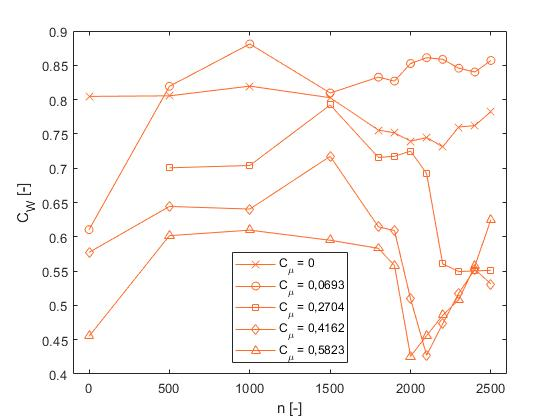
\includegraphics[width=0.5\textwidth]{Cw_ueber_n_fuer_verschiedeneCmu_50.jpg}
	\caption{$C_{w}$ "uber $n$ bei verschiedenen $C_{\mu}$ f"ur die Konfiguration 50}
	\label{fig:Cw/n bei Cmu 50}
\end{figure}

Die zus"atzliche Rotation der Walzen ist aber nur bei bestimmten $C_{\mu}$ und Drehzahlen widerstandsreduzierend. Bei allen $C_{\mu}$ wird der $C_{W}$ bei Beginn der Rotation erh"oht, bis er wieder im Bereich der Abl"osefrequenz einbricht. Allerdings ist die Sensibilit"at bei h"oheren $C_{\mu}$ in diesem Frequenzbereich sehr hoch, sodass der Widerstand deutlich erh"oht wird, wenn die optimale Drehzahl nicht getroffen wird. 
Bei der ersten Versuchsdurchf"uhrung mit der Ausblasug ($C_{\mu}$=0,069) "andert sich der Verlauf im Bereich der Abl"osefrequenz nur geringf"ugig. Dies kann daran liegen, dass der Materialabrieb den Spalt verstopft hat und die geringe Ausblasung nicht weg zu transportieren.


In der \abb{fig:CwCwref/n Cmu RK} sind die mit dem jeweiligen $C_{ref}$ normierten $C_{W}$-Werte der Basiskonfiguration, bei verschiedenen $C_{\mu}$ zu sehen.
Als jeweiliges $C_{ref}$ dient hierbei der $C_{W}$-Wert des entsprechenden $C_{\mu}$s ohne Rotation.


\begin{figure}[h]
	\centering
	\begin{subfigure}[c]{0.45\textwidth}		
		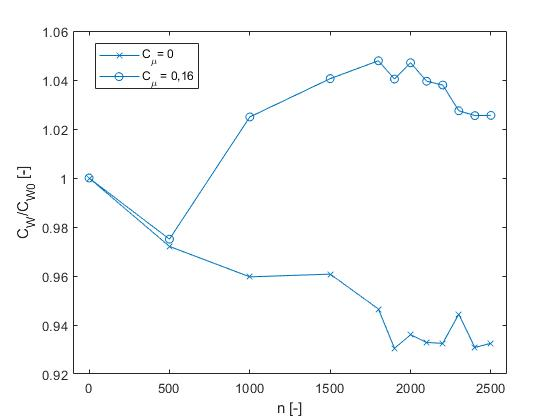
\includegraphics[width=1\textwidth]{CwCw0_ueber_n_fuer_2Cmus_RK.jpg}
		%\subcaption{}
	\end{subfigure}
	\begin{subfigure}[c]{0.45\textwidth}
		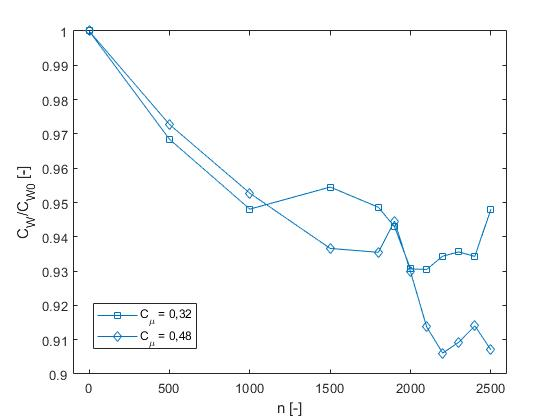
\includegraphics[width=1\textwidth]{CwCw0_ueber_n_fuer_Cmu3und4_RK.jpg}
		%\subcaption{}
	\end{subfigure}
	\begin{subfigure}[c]{0.45\textwidth}
		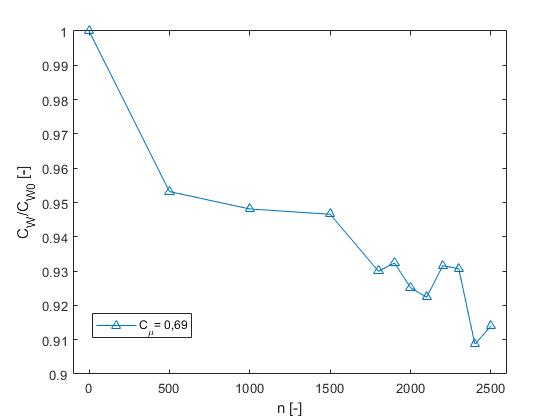
\includegraphics[width=1\textwidth]{CwCw0_ueber_n_fuer_Cmu5_RK.jpg}
		%\subcaption{}
	\end{subfigure}
	\caption{$C_{W}/C_{Wref}$ "uber n bei verschiedenen $C_{\mu}$ f"ur die Basiskonfiguration}
	\label{fig:CwCwref/n Cmu RK}
\end{figure}

In der \abb{fig:CwCwref/n Cmu 50} sind die mit dem jeweiligen $C_{ref}$ normierten $C_{W}$-Werte der Konfiguration 50, bei verschiedenen $C_{\mu}$ zu sehen.
Als jeweiliges $C_{ref}$ dient hierbei der $C_{W}$-Wert des entsprechenden $C_{\mu}s$ ohne Rotation.
Hier sehen die Verl"aufe au"ser bei einem $C_{\mu}$=0,16 "ahnilch aus und der normierte Widerstandsbeiwert sinkt mit erh"ohter Drehzahl insbesondere im Bereich der Abl"osefrequenz. 
Eine Drehzahlerh"ohung mit einer Ausblaseintensit"at von $C_{\mu}$=0,16 ist nur bis zu der Drehzahl n=500 effektiv. Danach steigt der Verlauf stark.

\begin{figure}[h]
	\centering
	\includegraphics[width=0.5\textwidth]{CwC0_ueber_n_fuer_Cmus_50.jpg}
	\caption{$C_{W}/C_{Wref}$ "uber n bei verschiedenen $C_{\mu}$ f"ur die Konfiguration 50}
	\label{fig:CwCwref/n Cmu 50}
\end{figure}

In der \abb{fig:PR} sind die Leistungsraten beider Konfigurationen bei verschiedenen Impulskoeffizienten und Drehzahlen ersichtlich.\\
Ein $PR= 1$ bedeutet, dass man so viel Energie mit der Widerstandsreduzierung erspart hat, wie man Energie f"ur dieselbe eingesetzt hat. In so einem Fall wird man sich in der Realit"at gegen diese widerstandsreduzierenden Ma\ss{}nahmen entscheiden, da diese nur erh"ohten Zeitaufwand, h"ohere Kosten und Reparaturanf"allifgkeit, ein gesteigertes Gewicht und weitere negative Nebenwirkungen zur Folge haben.

\begin{figure}[h]
	\centering
	\begin{subfigure}[c]{0.45\textwidth}		
		\includegraphics[width=1\textwidth]{PR_uber_n_fuer_Cmu_RK.jpg}
		\subcaption{$PR$ f"ur die Basiskonfiguration}
		\label{fig:PR RK}
	\end{subfigure}
	\begin{subfigure}[c]{0.45\textwidth}
		\includegraphics[width=1\textwidth]{PR_ueber_n_fuer_Cmu_50.jpg}
		\subcaption{$PR$ f"ur die Konfiguration 50}
		\label{fig:PR 50}
	\end{subfigure}
		\caption{$PR$ "uber $n$ bei verschiedenen $C_{\mu}$ f"ur beide Konfigurationen}
	\label{fig:PR}
\end{figure}

Es wird deutlich, dass die Konfiguration 50 bei keiner Drehzahl und keinem $C_{\mu}$ den Wert 1 erreicht, oder "uberschreitet. Der wichtigste zu nennende Grund daf"ur ist die gro\ss{}e Reibung zwischen der Teflonschicht und dem Ausblaseschlitz, die durch die Motoren "uberwunden werden muss. Diese aufzubringende Kraft ist unter anderem so gro\ss{}, da man gewisse Vorspannkr"afte aufbringen musste, um den vordefinierten Signalverlauf sicherzustellen.

Die Basiskonfiguration erreicht im Vergleich zu der gezahnten Konfiguration eine deutlich h"ohere Effektivit"at, auch wenn nicht immer vorteilhaft, da gerade nur bei zwei $C_{\mu}$s und einer Drehzahl bis ca. 1000\,$\mathrm{min^{-1}}$ Leistung erspart werden kann. Allerdings wird deutlich, dass die Bestwerte bei reiner Ausblasung erreicht werden. Die Widerstandsreduzierung der rotierenden Walzen verursacht einen gro\ss{}en energetischen Aufwand, sodass die Leistungsersparnis trotz einer Widerstandsreduzierung kleiner wird oder sogar in Leistungsverlust umgewandelt wird.
\chapter{Fazit (FT)}\label{s:fazit}
Im Rahmen dieser Projektarbeit wurde ein hybrider Aktuationsmechanismus auf eine m"ogliche Widerstandsreduktion an einem D-Stumpfk"orpermodell "uberpr"uft.
Der hybride Aktuationsmechanismus setzte sich dabei aus rotierenden Wellen und der Ausblasung von Coand\^{a}-Jets zusammen.
Im Fokus der Projektarbeit stand dabei die Frage, ob eine periodische Aktuation eine zus"atzliche Reduktion des Widerstands im Vergleich zur konstanten Aktuation bewirken kann und, ob dieser Mechanismus im Bezug auf die Leistungsbilanz sinnvoll eingesetzt werden k"onnte.

F"ur diese Zwecke wurden zwei "ahnliche, gezahnte Paare Walzen aus PTFE konstruiert und gefertigt, die f"ur eine eine periodische Ausblasung mit definiertem Signal und jeweils unterschiedlichen duty cyclen sorgen sollten. Ein Paar war wegen zu gro\ss{}er Fertigungsungenauigkeiten nicht f"ur die Versuche verwendbar.

Die Messdaten wurden "uber einen Druckmessrechen im LNB des ISM der TU Braunschweig bei verschiedenen Kombinationen der Ausblaseintensit"at und Walzenumdrehungen pro Minute gewonnen.

Im Anschluss wurden die Widerstandsbeiwerte  und verschiedene zugeh"orige Leistungskoeffizienten bestimmt und diese Daten hinsichtlich der Effektivit"at der Widerstandsreduktion und der Leistungsbilanz der einzelnen Konfigurationen, sowie m"oglichen Synergieeffekten ausgewertet.

Die Ergebnisse bez"uglich konstanter Aktuation von \textit{Bilges}, die eine Leistungsersparnis durch die Widerstandsreduktion bei einer begrenzten Zahl an Kombinationen der Aktuationsparameter im unteren Intensit"atsbereich festgestellt haben, konnten best"atigt werden. 

Es wurde zudem gezeigt, dass die periodische Aktuation im Bereich knapp oberhalb der nat"urlichen Abl"osefrequenz von 1938\,$\mathrm{min^{-1}}$ einen deutlichen positiven Einfluss auf die Reduktion des Widerstands des stumpfen K"orpers hat.

Allerdings zeigten die gefertigten gezahnten Wellen bei Rotation Abrieberscheinungen, die zus"atzlich in einer deutlich geschm"alerten  Leistungsbilanz m"undeten.
So stieg der Leistungskoeffizient $C_{Power}$ der Motoren  im Durchschnitt auf das etwa Dreifache im Vergleich zur Basiskonfiguration.
Eine weitere Schwierigkeit, die im Zuge der periodischen Aktuation auftrat, war, die Phasengleichheit der rotierenden Wellen an Ober- und Unterseite sicherzustellen.

So kann die ausg"angliche Fragestellung durch die Projektarbeit nicht abschlie\ss{}end gekl"art werden. Vielmehr ist es notwendig diese Art der aktiven Str"omungsbeeinflussung in zuk"unftigen Arbeiten mit mehreren Modifikationen erneut zu testen. Denkbar w"aren beispielsweise eine andere Auswahl bzw. Anordnung der  Materialien die an der Paarung von Spaltlippe und Welle beteiligt sind. Dar"uber hinaus muss in Zukunft die Phasensynchronisierung auf mechanische oder elektronische Weise gew"ahrleistet werden.


% Literaturverzeichnis
\newpage
\fancyhead[RE]{Literaturverzeichnis}
\fancyhead[LO]{Literaturverzeichnis}
\addcontentsline{toc}{chapter}{Literaturverzeichnis}
\bibliographystyle{plain}
%\bibliographystyle{bib_name_year}
\bibliography{lit_all} 


% Abbildungsverzeichnis
\newpage
\fancyhead[RE]{Abbildungsverzeichnis}
\fancyhead[LO]{Abbildungsverzeichnis}
{
   \renewcommand{\baselinestretch}{0.85}   %% Zeilenabstand / TOC
   \small\normalsize			   %% neuen Zeilenabstand aktivieren
   \addcontentsline{toc}{chapter}{Abbildungsverzeichnis}
   \listoffigures
}


% Tabellenverzeichnis
\newpage
\fancyhead[RE]{Tabellenverzeichnis}
\fancyhead[LO]{Tabellenverzeichnis}
{
   \renewcommand{\baselinestretch}{0.85}    %% Zeilenabstand / TOC
   \small\normalsize                        %% neuen Zeilenabstand aktivieren
   \addcontentsline{toc}{chapter}{Tabellenverzeichnis}
   \listoftables
}


% Anhang
\fancyhead[RE]{\nouppercase{\leftmark}}
\fancyhead[LO]{\rightmark}
\begin{appendix}
   \chapter{Technsiche Zeichnungen (NB, TG)}\label{s:anh_TZ}

\includepdf[angle=90]{./figures/DrawingInnenwelle.pdf}
\includepdf{./figures/Mantel_A.pdf}
\includepdf{./figures/Mantel_B.pdf}
   \chapter{MATLAB-Code (AK, FT)}
\label{c:Anhang B}

\section{Bestimmung der Druckverteilungen und des Widerstands}
\label{C_w-Code}
\begin{figure}[h]
	\centering
	\includegraphics[width=1\textwidth]{wake_n-1.jpg}
	\label{fig:C_w-Code}
\end{figure}
\begin{figure}
	\centering
	\includegraphics[width=1\textwidth]{wake_n-2.jpg}
\end{figure}
	
	
\end{appendix}

\end{document}
